%===============================================================================
% Autoři šablony: Michal Bidlo, Bohuslav Křena, Jaroslav Dytrych, Petr Veigend a Adam Herout 2018
% Autor práce: Jakub Chlebík
\chapter{Úvod}
\label{intro}
Evoluční algoritmy jsou moderním způsobem řešení náročných optimalizačních problémů, pro které doposud neexistuje přesná, matematickou analýzou podložená, metoda. Jsou součástí tématu nazývaného anglicky \uv{Soft Computing}, od ostatních metod této rodiny se ovšem liší svou tolerancí nepřesností a šumu, schopností pracovat s~aproximacemi a jistou náhodností.

Cílem práce je statistickou analýzou nalézt takový evoluční algoritmus, který dle vybraných kritérií nejlépe navrhne plán ulrazvukové operace. V~tomto textu bude představeno několik vybraných evolučních algoritmů, otestována jejich schopnost hledat optimum nad vhodnou testovací sadou a diskutována jejich vhodnost pro optimalizaci hledání ultrazvukové trajektorie. Následně jsou tyto algoritmy aplikovány na model šíření tepelné energie a představeny statistické výsledky.  Jak již je u~optimalizačních problémů složitějších systémů zvykem, i zde platí tzv. \uv{No Free Lunch}~teorém a je tedy třeba podstoupit jisté kompromisy. Ty jsou vyjádřeny formou kritérií, dle kterých jsou algoritmy hodnoceny.

V~následující kapitole je představen problém optimalizace plánů systému ultrazvukových operací. Zde budou prezentována kritéria, kterými je třeba se řídit při hodnocení vhodnosti jednotlivých optimalizačních metod. Diplomová práce navazuje na článek~\cite{FITPUB11696}, jehož stěžejní body budou v~následující kapitole představeny. V~kapitole 3 budou detailněji popsány jednotlivé zkoumané algoritmy - principy jejich fungování, motivace k~jejich vzniku a kladné i stinné stránky použití. Jedná se o~optimalizační metody \textit{genetického algoritmu},\textit{simulovaného žíhání}, \textit{metoda tabu prohledávání}, \textit{optimalizace rojem částic}, \textit{diferenciální evoluce} a \textit{evoluční strategie založená na adaptaci kovarianční matice}. Kapitola 4 představí implementaci jednotlivých algoritmů, jejich rozhraní a výstupní protokol. Následně je představeno několik typických problémů pro hodnocení optimalizačních metod a statistickým způsobem ukázáno, jak dobře byly schopny zmíněné vybrané algoritmy tyto optimalizační testy řešit. V~závěru kapitoly je provedeno zběžné zhodnocení implementovaných optimalizačních metod pro řešení problémů v~testovací sadě a představena kritéria hodnocení těchto metod v~kontextu optimalizace trajektorie HIFU operací. Kapitola 5 se bude věnovat samotné simulaci šíření tepla. Představí testovací sadu několika modelů cílené tkáně pro ablaci, které jsou založeny na získaných poznatcích o~problému optimalizace trajektorie. Následně jsou provedeny experimenty a výsledky statisticky prezentovány a zhodnoceny. V~závěru je poté vybráno několik vhodných algoritmů pro další studium.

\chapter{Optimalizovaný systém}
\label{about}
Následující kapitola si klade za cíl seznámit čtenáře se systémem HIFU - Fokusovaný ultrazvuk o~vysoké intenzitě. Se svolením autora je téměř celý obsah této kapitoly, včetně obrázků~\ref{focalRegion},~\ref{fg:austinWoman} a~zdrojů~\cite{BLOODOCCLUSION},~\cite{HIFUTHERMALMODEL},~\cite{HIFUPropagation} převzat, přeložen a nebo parafrázován ze článku~\texttt{Design of HIFU Treatment Plans using an Evolutionary Strategy}~autorů \textit{Jiří Jaroš, Marta Jaroš} a~\textit{Bradley E. Treeby}~\cite{FITPUB11696}. Toto dílo se má práce snaží rozšířit a~je tedy vhodné jej zde i~představit. Nejdříve je ovšem třeba udělat krok zpět a~představit pojmy optimalizace a operační výzkum - této problematice jsem se již věnoval ve své bakalářské práce~\cite{Chlebik2017} a proto zde i uvádím původní část tohoto textu.

\section{Matematická optimalizace} \label{subsec:MatOpt}
Optimalizace je podoborem matematické analýzy a numerické matematiky, zabývající se hledáním extrému zobrazení \(f: \mathbb{R}^n \rightarrow \mathbb{R}\) v~prostoru \(\Omega = \mathbb{R}^n\). Přesněji, vyhledává množinu vstupních parametrů \( x = x_{1}, ... , x_{n} \) problému, které odpovídají minimu, případně maximu, hodnotící funkce \( f(x) = f(x_{1}, ... , x_{n})\).

\theoremstyle{definition}
\newtheorem{definition}{Definice}
\theoremstyle{definition}
\begin{definition} {Minimum funkce.\\}
Nechť \(f: \mathbb{R}^n \rightarrow \mathbb{R}\) je funkce \(n\) proměnných. Tvrdíme, že \(x^* \in \mathbb{R}\) je minimem \(f\) (dále v~textu pouze "minimum"), pokud existuje \(\delta > 0\) taková, že pro všechna \(x\) ve vztahu 
\(\Vert x - x^* \Vert \leq \delta\) platí
\(f(x^*) \leq f(x)\). Analogicky lze odvodit definici maxima.
\label{def:minim}
\end{definition}

O~takovémto minimu tvrdíme, že je lokálním, pokud je nejmenším bodem v~daném okolí. O~globálním minimu hovoříme, pokud je takovýto bod nejmenším na celém definičním oboru. Znázorněno na obrázku~\ref{fig:localGlobal}.

Díky vztahu 
\begin{equation}
\max\limits_{x \in \Omega}(f (x)) = -\min\limits_{x \in \Omega}(-f(x))
\label{eq:max_min}
\end{equation} 
můžeme vždy předpokládat, že optimalizační problém je problémem minimalizačním a maximalizací se dále nemusíme zabývat. 

\begin{figure}
\centering
\includegraphics[width=\linewidth * 3/4]{obrazky-figures/localGlobal.png}
\caption{Ukázka globálního a lokálního minima na jednoduché matematické funkci. Zdrojem je internet.}
\label{fig:localGlobal}
\end{figure}


\subsection{Klasifikace optimalizačních úloh} \label{subsec:classific}
Dle definičního oboru prostoru \(\Omega\) účelové funkce se optimalizační úlohy klasifikují na:

\begin{itemize}
\item Úlohy volného extrému. Tento případ nastává, pokud \(\Omega = \mathbb{R}^n\).
\item Úlohy vázaného extrému - případ kdy \(\Omega \subset \mathbb{R}^n\). Zde nás zajímají pouze řešení, která splňují další podmínky, omezující buďto jeden nebo více vstupních parametrů \(x_0, ... x_n\) na interval, nebo funkcemi \(g_0(x_i, ... x_n) \geq 0 \). O~takto definovaných úlohách se mluví jako o~úlohách matematického programování. Jednoduché příklady omezení vázaného extrému jsou znázorněna na obrázcích~\ref{fig:BoxConstraint} a~\ref{fig:GeneralConstraint}.
\item Funkce jednoho extrému - tzv. \uv{unimodální}.
\item Funkce více extrémů stejné váhy - tzv. \uv{multimodální}.
\end{itemize}

\begin{figure}[!tbp]
\begin{minipage}[b]{0.450\linewidth}
\includegraphics[width=\linewidth]{obrazky-figures/box_constraint.png}
\caption{Omezení intervalem.}
\label{fig:BoxConstraint}
\end{minipage}
\hfill
\begin{minipage}[b]{0.450\linewidth}
\includegraphics[width=\linewidth]{obrazky-figures/general_constraint.png}
\caption{Omezení funkcí.}
\label{fig:GeneralConstraint}
\end{minipage}
\end{figure}

\subsection{Operační výzkum} \label{subsec:OpRes}
Pojmem \emph{operační výzkum} (často označován také jako operační analýza) se všeobecně rozumí převod komplexní inženýrské úlohy reálného světa na matematický, či jiný, model a následné provádění experimentů pro získání informací. Problémy tohoto typu jsou často spojeny s~hledáním minima (např. provozní riziko), maxima (např. zisk), či jiného optimálního výsledku. Teoretickým základem operačního výzkumu je tedy matematická optimalizace a ke hledání řešení se využívá metody optimalizací, modelování a simulací~\cite{operResearch}.

Průběh operačního výzkumu je znázorněn na obrázku~\ref{fig:Operation_Research}. \\
\begin{figure}[h]
\centering
\includegraphics[width=\linewidth * 3/4]{obrazky-figures/operacniVyzkum.pdf}
\caption{Zjednodušený náhled na proces operačního výzkumu}
\label{fig:Operation_Research}
\end{figure}


\section{Fokusovaný ultrazvuk o~vysoké intenzitě}
\label{about:sec:hifu}
Fokusovaný ultrazvuk o~vysoké intenzitě je moderní technika pro ne-invazivní operace nádorových onemocnění, při které je maligní tkáň odstraněna kumulovanou tepelnou energií vyzářenou ultrazvukovými vysílači. Tato takzvaná termální ablace je provedena pod dohledem profesionála a úkolem je zvýšit teplotu v~cíleném místě o~několik desítek stupňů, čímž dojde ke zničení tkáně. Na rozdíl od standardních postupů léčby rakoviny se jedná o~ne-invazivní a ne-ionizující řešení, které již bylo aplikováno ve více než 100,000 případech.

Jedno toto ultrazvukové ozáření - tzv. sonikace - dokáže odstranit pouze malou oblast cílené tkáně. V~závislosti na velikosti oblasti ošetřované části může být potřeba absolvovat sérii těchto sonikací (běžně v~řádu desítek). Každá takováto sonikace může způsobit různá další zranění - od popálenin kůže až po možné vážné poškození tkáně poblíž fokálního místa a nebo někde mezi vysílačem a nádorem.

Hlavním problémem tohoto přístupu je tedy toto: jak rozmístit sérii ohnisek vysílačů v~prostoru tak, aby se minimalizovalo riziko zranění i počet sonikácí a zároveň byla zničena všechna nežádoucí tkáň. Navíc je třeba dát pozor na různé komplikace, jako například krevní řečiště sousedící s~cíleným tumorem, které může odvést velkou část indukované tepelné energie, nebo může být zářením poškozeno~\cite{BLOODOCCLUSION}. Série ohnisek sonikací poté vytváří trajektorii. Toto je optimalizační, přesněji minimalizační, problém, který svou povahou připomíná problém batohu - snažíme se co nejmenší vahou (zatížením těla sonikacemi) zaplnit co největší prostor (odstranit celou nežádoucí tkáň). Bohužel, běžné matematicko-fyzikální rovnice pro šíření zvukových vln a tepla spolu s~metodami optimalizace v~tak komplikovaném a heterogenním prostředí, jako může být i lidský mozek, a pro tak individuální systém selhávají, a je třeba přistoupit k~metodám operační analýzy a soft comuputingu - heuristiky a nebo algoritmy umělé inteligence. Tento přístup obětuje exaktní přesnost za rychlejší proces s~možností opakované, parametrizovatelné simulace spolu se zpětnou verifikací.



\begin{figure}[hbt]
	\centering
	\includegraphics[width=0.7\textwidth]{obrazky-figures/ohnisko.png}
	\caption{Vizualizace regionů, ve kterém se indukuje teplo v~závislosti na vzdálenosti ohniska od vysílače. Převzato z~\cite{FITPUB11696}.}
	\label{focalRegion}
\end{figure}

\section{Rozšiřované řešení}
\label{about:sec:existSolution}
Jak již bylo nastíněno, k~řešení tohoto problému je třeba vytvořit model pro šíření tepla ve tkáních. Takovýto model byl již implementován v~nástroji k-Wave~\cite{HIFUTHERMALMODEL} a~využit v~řešení~\cite{FITPUB11696}.

\subsection*{Model} 
Průběh simulace modelu se skládá z~několika stádií. V~následujícím výpisu pouze nastíním jejich funkci, pro detailnější popis včetně referencí doporučuji již zmíněnou zdrojovou práci~\cite{FITPUB11696}:
\begin{itemize}
    \item \textit{Výpočet přidané tepelné energie ve tkáni} - v~závislosti na délce sonikace, pozici, velikosti a tvaru ohniska (znázorněno na obrázku~\ref{focalRegion}) je třeba zjistit, kolik tepelné energie bude vydáno zářením. Přesné výpočty jsou možné například za použití modelu ~\cite{HIFUPropagation}. Bohužel, tyto modely jsou příliš výpočetně náročné pro efektivní použití optimalizační metody, především pak pro použitou evoluční metodu. Proto bylo zavedeno několik zjednodušení a předpokladů. Tyto alternace jsou řádně ocitovány v~již zmíněném článku~\cite{FITPUB11696}.
    \item \textit{Šíření a rozptyl tepla ve tkáni} - dále je třeba zjistit, jak se všechno přidané teplo rozšířilo ve tkáních. Jedná se o~model Penneho biotepelné rovnice šíření, jejíž simulace je prováděna v~nástroji k-Wave~\cite{HIFUTHERMALMODEL}. Výstupem tohoto modelu je prostorová termální mapa (tzv. $CEM_{43}$ - Cumulative Equivalent Minutes at 43$^{\circ}$) kumulovaného tepla za sérii sonikací.
    \item \textit{Přesnost řešení}  - tato tepelná mapa je v~posledním kroku převedena na binární masku podle hranice. Následně je spočten integrál nad celou touto mapou, sčítající hodnoty oblastí, které byly ošetřeny a neměly být, spolu s~hodnotami oblastí, které neměly být ošetřeny a byly. Dále byla zavedena nevýznamná oblast - oblast ve které nás možná abraze nezajímá. Názorně zobrazeno na obrázku~\ref{fg:austinWoman}.
\end{itemize}

\subsection*{Plánování trajektorie}
K~návrhu a optimalizaci plánu byl použit algoritmus \uv{Covariance Matrix Adaptation - Evolutionary Strategy} - zkráceně CMA-ES. Jedná se o~moderní variantu evoluční strategie, pro nelineární nekonvexní systém černé skříňky definované na spojité veličině. Nevyžaduje náročné ladění parametrů - naopak výběr strategie vnitřních parametrů si algoritmus zvolí a postupně vylepšuje sám. Více se tímto algoritmem zabývá sekce~\ref{algs:cmaes}.

\subsection*{Kódování řešení}

Dále bylo také již navrženo kódování hledaných parametrů do chromozomu. Kandidátní řešení $I$ je poté trajektorie sonikací, kde $i$ odpovídá pořadí sonikací~\cite{FITPUB11696}: 
\begin{equation}
    \label{eq:trajectory}
     I~= (S_{1}, S_{2}, ..., S_{N})
\end{equation}kde
\begin{equation}
    \label{eq:S}
     S_{i} = (x(i), y(i), t_{on}(i), t_{off}(i)) 
\end{equation}
\begin{itemize}
    \item $S_i$ - parametry sonikace $i$
    \item $x(i), y(i)$ - 2D souřadnice ohniska sonikace $i$
    \item $t_{on}(i)$ - délka sonikace $i$
    \item $t_{off}(i)$ - interval ochlazení po dokončení sonikace $i$
\end{itemize}

\begin{figure}[hbt]
	\centering
	\includegraphics[width=0.7\textwidth]{obrazky-figures/austinWoman.png}
	\caption{Segmentová mapa AustinWoman s~vyznačenou cílovou, zakázanou a nevýznamnou oblastí. Převzato z~\cite{FITPUB11696}.}
	\label{fg:austinWoman}
\end{figure}


%https://www.kiv.zcu.cz/studies/predmety/uir/gen_alg2/E_alg.htm
%https://ieeexplore.ieee.org/stamp/stamp.jsp?tp=&arnumber=7955308
%https://www.vutbr.cz/www_base/zav_prace_soubor_verejne.php?file_id=31876
%https://wis.fit.vutbr.cz/FIT/st/cfs.php?file=%2Fcourse%2FEVO-IT%2Flectures%2F04-GenetickeAlg.pdf&cid=12093
\chapter{Evoluční algoritmy} 
\label{algs}
\textit{Evoluční algoritmy} (zkráceně EA) patří do kategorie přírodou inspirovaných algoritmů. Jedna se o~zastřešující množinu pro různé přístupy, které se inspirují v~evolučním procesu - pokud je populace jedinců vystavena dlouhodobě selekčnímu tlaku, začíná se v~následujících generací na tento tlak lépe adaptovat, aby druh přežil. Takto adaptovaní jedinci dále šíří své geny a neustále vylepšují zdatnost následujících populací. Z~technického pohledu je množina jedinců (generace) iterativně vystavována evolučním operacím (v~genetickém algoritmu jsou to operace selekce nejlepších jedinců, jejich křížení a případně mutace potomků) pro vytvoření generace nové. Zda-li se původní jedinci budou či nebudou nacházet v~nové populaci již záleží na implementaci samotné. 

Z~matematického hlediska se řadí mezi stochastické metody prohledávání stavového prostoru a \textit{metaheuristiky} - strategie, či procedura na nějaké vyšší úrovni, jejíž cílem je nalézt proceduru nebo heuristiku o~úroveň níže, která bude schopná řešit zadaný problém bez bližších údajů o~optimalizovaném systému~\cite{EA_OVERVIEW}.

Již mnohokrát se ukázalo, že EA dokáží najít inovativní či zcela nová řešení inženýrských úloh, která konvenční algoritmy nejsou schopna poskytnout~\cite{EVO}. \\

\noindent Oproti konvenčním optimalizačním metodám vykazují EA především tyto vlastnosti:
\begin{itemize}
    \item Výhody \begin{itemize}
         \item Jednodušší a flexibilnější návrh - není třeba pokročilých znalostí matematiky či fyzikálních principů k~použití těchto algoritmů.
         \item Umožňují optimalizovat systémy o~kterých nemají žádné informace. 
        \item Pokud ovšem tyto informace máme, jsme schopni je využít ke zrychlení/zefektivnění optimalizace.
        \item Robustnost a schopnost přizpůsobit se změnám v~prostředí či prostředí samotného a šumu.
        \end{itemize}
    \item Nevýhody \begin{itemize}
        \item Samotná povaha metod je stochastická a tedy nezaručuje optimálnost řešení.
        \item Algoritmy této rodiny jsou často velice náchylné na nastavené parametry a špatné zvolení těchto parametrů vede na selhání.
        \end{itemize}
\end{itemize}

Další rodina algoritmů, která se do skupiny evolučních algoritmů zařadila nedávno, se nazývá \textit{Memetické algoritmy}, nebo také kulturní algoritmy či genetické lokální prohledávání~\cite{EA_OVERVIEW}. Na rozdíl od evoluce celých populací se zaměřují na evoluci jedinců - selekčním tlakem zde není schopnost přežití v~přírodě nýbrž ve společnosti.

\begin{figure}[hbt]
	\centering
	\includegraphics[width=0.85\textwidth]{obrazky-figures/memetic.png}
	\caption{Memetické algoritmy. Převzato z~\cite{EA_OVERVIEW}}
	\label{fg:memtic}
\end{figure}

\subsection*{Selekční tlak}
Při prohledávání stavového prostoru je neustále třeba hledat rovnováhu mezi prohledáváním a \uv{vykořisťováním}~\cite{EVO}. Prohledávání nutí jedince v~populaci pokrýt celou plochu prohledávaného prostoru a vykořisťování umožní jedincům specializovat se v~nějaké podoblasti prostoru a skutečně konvergovat k~optimálnímu řešení v~tomto podprostoru~\cite{Weisser2010}. Tato síla se nazývá selekční tlak a pohání každý EA. Velikost selekčního tlaku ovlivňuje tendence algoritmu prohledávat a vykořisťovat. Čím větší je selekční tlak, tím menší stavový prostor algoritmus prohledává a tím více je hnán ke konvergenci k~optimu v~tomto podprostoru a naopak~\cite{Weisser2010}.

\subsection*{Pojmy}
Následuje výčet a vysvětlení používaných pojmů v~evolučních algoritmech~\cite{EVO}. Tyto pojmy mají svůj základ v~biologii, přesněji v~DNA a RNA~\cite{EA_OVERVIEW}:
\begin{itemize}
    \item \textit{Fenotyp/jedinec} - objekt a potencionální řešení daného problému.
    \item \textit{Chromozom/genotyp} - struktura řešení pro algoritmus. Konkrétní podoba chromozomu představuje jeden stav prohledávaného prostoru. Jeho interpretací získáváme fenotyp.
    \item \textit{Gen} - element chromozomu .
    \item \textit{Alela} - hodnota genu.
    \item \textit{Lokus} - pozice genu v~chromozomu.
    \item \textit{Populace} - struktura $n$ chromozomů. Multimnožina.
    \item \textit{Generace} - jedna iterace. Každá generace má svou populaci, na kterou jsou v~průběhu generace aplikovány genetické operátory. Výsledkem těchto operací je nová populace.
    \item \textit{Genetické operátory} - způsob a postup tvorby potomků z~rodičovských chromozomů.
    \item \textit{Ukončovací podmínky} - podmínka, při které je evoluce prohlášena za dokončenou. Typicky dosažení požadovaného výsledku nebo dosažení maximálního počtu generací.
    \item \textit{Fitness funkce} - funkce vyhodnocující  stupeň adaptace jedince s~ohledem na kritéria a cíle evolučního procesu, zjednodušeně schopnost jedince přežít.
    \item \textit{Prohledávaný prostor} - množina všech potencionálních řešení problému. Každý bod v~tomto prostoru má jistý potenciál pro přežití; svou fitness. Velikost a tvar tohoto prostoru je závislý na množině potencionálních řešení optimalizovaného problému. Zároveň ze znalosti řešeného problému mohou vyplynout další podmínky, které tento prostor dále omezí - tzv. omezující podmínky. Tato omezení nemusí a často nebývají lineární - například omezení křivkou nelineární funkce derivace některé z~proměnných.
\end{itemize}

Příklad: Pokud je fenotypem ASCII znak, chromozomem bude struktura osmi bitů, genem bit, alela bude hodnota 1 či 0 a lokus bude pozice zvoleného genu v~rámci znaku (0 - 7).

\section{Genetický algoritmus}
\label{algs:ga}
Genetický algoritmus (GA) je jedním z~nejpopulárnějších z~rodiny EA. Byl inspirované Darwinovou teorii evoluce a jako první jej popsal John Holland v~roce 1975~\cite{GAIntro}. Často je používán při strojovém učení, rozpoznávání a klasifikace a pro optimalizace. GA je populačně zaměřený EA a jako evoluční operace používá křížení a mutaci. Genetický algoritmus je běžný ve dvou variantách:
\begin{itemize}
    \item \textit{Generační model}, v~literatuře často \uv{generation GA} - vždy je celá populace jedinců nahrazena následující populací.
    \item \textit{Ustálený model}, v~literatuře \uv{steady-state GA} - v~každé generaci je nahrazován jen nejhorší jedinec.
\end{itemize}

\bigskip

Algoritmus začíná s~nějakou, typicky náhodně vygenerovanou, populací chromozomů. Každý jedinec populace je jedním řešením daného problému a principem je postupně se v~průběhu generací za pomoci genetických operátorů dostávat k~novým a kvalitnějším jedincům. Ohodnocení kvality každého z~jedinců probíhá za pomoci fitness funkce, která je specifická pro řešený problém. Toto je prováděno do té doby, dokud není splněno nějaké ukončovací kritérium. Flowchart~\ref{fg:gaFlow} ukazuje rozhodovací proces algoritmu.\\

\begin{figure}[hbt]
	\centering
	\includegraphics[width=0.6\textwidth]{obrazky-figures/gaFlow.pdf}
	\caption{Flowchart průběhu genetického algoritmu.}
	\label{fg:gaFlow}
\end{figure}

\subsection{Kódování chromozomu}
Jedná se o~způsob, jakým je reprezentována struktura chromozomu. Lze uvažovat například kódování binární - 8 bitů tvoří chromozom a každý bit je jedním genem. Nebo také ale bity nemusí být pro nás významnou hodnotou a chromozomem je například binární strom, či seznam prvků nebo i~obyčejné číslo (reálné nebo i přirozené). 

\subsubsection*{Binární kódování}
Původní varianta GA používala právě toto kódování. Typickým případem použití tohoto kódování jsou problémy, jejichž jedinci nejsou definováni na množině čísel, případně potřebujeme velkou kontrolu nad evolucí jedinců. Nevýhodou použití tohoto kódování pro číselné~typy, respektive typy, na nichž je definována relace uspořádání je tzv. \textit{Hammingova bariéra} - malá změna v~genotypu jedince může způsobit velké změny fenotypu. Například čísla $127d = 01111111b$ a $128d = 10000000b$. Toto může snižovat výkonnost algoritmu~\cite{Weisser2010}. Jedním z~možných řešení je tzv. \textit{Grayův kód} - binární kódování čísel, ve kterém se sousední hodnoty vždy liší pouze v~jednom bitu. Pro ukládání reálných čísel je nejdříve třeba tyto čísla převést na celá čísla. 

\subsubsection*{Číselné}
Typicky používáno pro optimalizační úlohy definované na množině $\mathbb{N}$ či $\mathbb{R}$. V~takovýchto úlohách se běžně pracuje s~číselnými fenotypy a není třeba nižší úrovně ukládání hodnot. Dalším příkladem použití celočíselných chromozomů je \textit{pořadové kódování}, které se používá pro úlohy hledání cest. Poté může být každý uzel reprezentován jedním číslem a~chromozom obsahovat seznam čísel, jejichž pořadí udává pořadí, ve kterém jsou uzly navštíveny.


\subsection{Selekce}
Představuje postup, jakým jsou vybírány chromozomy aktuální populace pro proces křížení~\cite{EVO, Weisser2010}. Následně jsou uvedeny nejběžněji používané selekční operátory.

\subsubsection*{Turnaj}
Náhodně vybráno $m$ jedinců, kteří se účastní turnaje. Vítěz tohoto turnaje je poté vybrán pro křížení. Podmínky pro vítězství v~turnaji se mohou lišit, typické je ovšem použít hodnotu fitness. 

\subsubsection*{Vážená ruleta}
Pravděpodobnost výběru každého jedince závisí na jeho fitness hodnotě a na fitness hodnotě zbytku populace. Představme si ruletu, kterou roztáčíme pokaždé, když chceme vybrat jedince. Čím lepší fitness má jedinec vzhledem ke zbytku populace, tím větší je jeho část rulety a tedy tím větší šanci má, že bude vybrán~\cite{EVO, Weisser2010}.

\subsubsection*{Rank}
Jedinci v~populaci jsou seřazení podle své fitness od nejlepšího k~nejhoršímu. Každému jedinci je přiřazeno číslo $k$, které například určuje, kolik jedinců v~populaci je horších, než je on sám. Následně je dle tohoto čísla spočítána pravděpodobnost každého jedince k~výběru~\cite{EVO, Weisser2010}.

\subsubsection*{Elitismus}
Nejlepšího jedinec (případně $n$ nejlepších) přežije svou generaci a dostane šanci uplatnit se v~následující. Takovýto jedince přeskakuje evoluční operátory. Elitismus má potenciál snižovat diverzitu populace a naklánět selekční tlak spíše k~vykořisťování~\cite{EVO}. Jedná se o~emergentní~\ref{def:emergence} vlastnost některých selekčních operátorů. V~případech, kdy nepoužíváme tyto operátory, můžeme tuto vlastnost algoritmu zavést explicitně. 

\subsubsection*{Incest}
Jedince s~podobnými chromozomy lze považovat za příbuzné a pokud by mělo dojít ke křížení takovýchto jedinců, nevznikne žádná nová vlastnost. Tento jev snižuje diverzitu populace a může vést k~předčasné konvergenci a je třeba se mu bránit. Tuto situaci lze detekovat za pomoci \textit{Hammingovy vzdálenosti}, případně \textit{Euklidovské metriky}. Pokud jsou dva jedinci vybraní k~páření příbuzní, je třeba zamezit křížení a provést selekci nového jedince~\cite{Weisser2010}.

\subsection{Křížení}
Je kombinací rodičovských genů za cílem vytvoření potomstva. Má význam pro zvýšení schopnosti explorace algoritmu a zajištění diverzity, ovšem také ke schopnosti algoritmu konvergovat. Spolu s~vhodnou selekční metodikou tlačí populaci k~jedincům s~lepšími vlastnostmi. V~základním provedení 2 rodiče produkují 2 potomky. Následující varianty operace křížení předpokládají standardní binární či celočíselnou reprezentaci. Pokročilejší zakódování vyžadují speciální návrhy těchto operátorů. V~případě číselných chromozomů je možné pro křížení použít například operace průměru či sečtení~\cite{EVO, Weisser2010}. 

\begin{figure}[!tbp]
\begin{minipage}[b]{0.485\linewidth}
\includegraphics[width=\linewidth]{obrazky-figures/cross_onepoint.pdf}
\caption{Jednobodové křížení.}
\label{fig:EA_1Cross}
\end{minipage}
\hfill
\begin{minipage}[b]{0.485\linewidth}
\includegraphics[width=\linewidth]{obrazky-figures/cross_multipoint.pdf}
\caption{Vícebodové křížení.}
\label{fig:EA_2Cross}
\end{minipage}
\end{figure}

\subsubsection*{Jednobodové}
V~chromozomech o~délce $n$ je náhodně zvolen index $i, 1 \leq i \leq n$. Prvních $i$ genů je poté získáno z~prvního rodiče, zatímco $i$ až $n$ z~druhého rodiče. Záměnou pořadí rodičů můžeme získat až dva potomky~\cite{Chlebik2017}. Znázorněno na obrázku~\ref{fig:EA_1Cross}.

\subsubsection*{Vícebodové}
Analogicky k~jednobodovému křížení, je vygenerováno až $k$ různých indexů $(i_0, ... i_k)$, pro které platí $(1 \leq i_1 \le i_2 \le ... \le i_k \le n)$. Poté se vybere náhodný rodič, ze kterého je zkopírována část $i_j$ až $i_{j+1}$, posune se index $j$ a rodiče alternují. Záměnou pořadí je i zde možné získat dva potomky~\cite{Chlebik2017}. Znázorněno na obrázku~\ref{fig:EA_2Cross}.
 
\subsubsection*{Uniformní}
Každému genu je vygenerována rovnoměrným rozložením zvoleno, ze kterého z~rodičů bude gen zkopírován. Záměna rodičů opět umožní získání druhého potomka.


\subsection{Mutace}
Klíčový genetický operátor z~pohledu přínosu nových vlastností jedinců~\cite{EVO, Weisser2010}. Obvyklým postupem je zcela náhodná změna několika náhodně vybraných genů u~náhodně vybraných jedinců. Smyslem mutace je zvyšovat diverzitu populace. Pravděpodobnost výskytu mutace se typicky volí jako nízká; při neúměrně vysoké mutaci totiž může docházet k~narušování dříve slibných řešení před konvergencí k~optimu. Ovšem příliš nízká mutace může vést na nedostatečnou diverzitu populace a s~tím spojené omezené schopnosti GA prohledávat stavový prostor.
V~binárních chromozomech můžeme náhodně měnit bity, v~číselných například náhodně přičíst konstantu nebo vynásobit chromozom nějakou váhou či maskou~\cite{Chlebik2017}.

\section{Simulované žíhání}
\label{alg:sa}
Metoda simulovaného žíhání patří mezi memetické algoritmy a její základ je v~metalurgii, přesněji ve fyzikálním jevu žíhání - procesu, při kterém je těleso umístěno do pece vyhřáté na vysokou teplotu a~postupným pomalým ochlazováním jsou odstraňovány vnitřní defekty tělesa. Po dokončení je ocel stejně pevná ovšem ohebnější a~odolnější vůči poškození.

Při vysokých teplotách je těleso v~tekutém stavu, krystalová mřížka náhodně uspořádána s~krystalky kmitajícími v~prostoru - systém je ve stavu vysoké entropie. Postupným ochlazováním se celková entropie systému snižuje - krystalky mřížky přestávají kmitat a~pomalu se usazují do pozic s~nižší energií. Celý systém se tak dostává do rovnovážného stavu s~pevnou mřížkou bez defektů.

Algoritmus simulovaného žíhání následuje tento princip. Tělesem je náš optimalizovaný systém, u~kterého se předpokládá, že začíná ve stavu vysoké entropie. Kandidátní řešení algoritmu je potom energie systému, přesněji uspořádání krystalků mřížky. 
Postupem času se systém ochlazuje dle nějakého předem zvoleného chladícího rozvrhu a~mřížka se ustaluje - v~každém kroku jsou zaváděny náhodné poruchy momentálního stavu (je prohledáváno blízké \uv{okolí} současného stavu) a~je porovnávána energie při těchto defektech s~energií momentální. V~případě, že některá z~poruch má nižší energii, než stav momentální, určí jej algoritmus za nejlepší řešení v~rámci této iterace a~přijme jej za nový výchozí stav. V~případě, že se nenašel lepšího kandidáta, je proveden test na \textit{Metropolisovo kritérium}. Pokud je test úspěšný je i~horší stav přijat za momentální. Toto kritérium je založeno na Boltzmannové pravděpodobnostním rozdělení a~šance na přijetí klesá spolu s~teplotou~\cite{fitWebSA}: 

\begin{equ}[!ht]
\begin{equation}
\label{eq:boltz1}
W_T(E_i) = \frac{1}{Z(T)}\exp(\frac{-E_i}{k_BT})
\end{equation}
\end{equ}
kde  $T$ je teplota žíhaného tělesa, $E_i$ je energie systému ve stavu $i$, $k_B$ je Boltzmannova konstanta. Partiční funkce Boltzmannova rozdělení $Z(T)$ je rovnice \ref{eq:boltz2}:
\begin{equ}[!ht]
\begin{equation}
\label{eq:boltz2}
Z(T) = \sum_{j}\exp(\frac{-E_j}{k_BT})
\end{equation}
\end{equ}
\\
Znázorněno na obrázku \ref{fg:cooling}.

\subsection{Boltzmannovo rozdělení}
Za podmínky, že proces ochlazování je dostatečně pomalý je žíhaný systém vždy rovnovážném stavu - tento jev popisuje \textit{Boltzmannovo rozdělení pravděpodobnosti} (rovnice \ref{eq:boltz1} a~\ref{eq:boltz2}). V~případě, kdy dochází k~ochlazování systému příliš rychle mohou defekty zamrznout a vzniknout tak metastabilní struktury - lokální minima - které SA nedokáže překonat ~\cite{fitWebSA}. Pro simulaci tohoto rozdělení lze použít, a~v~metodě simulovaného žíhání se používá, algoritmus \textit{Metropolis}, který je implementací metody \textit{MCMC - Markov Chain Monte-Carlo}~\cite{webMCMC}.


\subsection{Monte Carlo a Markovské řetězce}
Monte Carlo je stochastická numerická metoda pro získávání znalostí o~simulovaných systémech pracující s~teorií pravděpodobnosti. Metoda provádí $n$ náhodných pokusů se systémem a po dokončení statisticky odhaduje charakteristiku systému. Metoda \textbf{Monte Carlo} je modelování takové náhodné veličiny $X$, že její střední hodnota $E(X)$ je rovna hledané hodnotě $a$. Pak, jestliže vypočteme $n$ nezávislých realizací $X_1, ..., X_n$ náhodné veličiny $X$, můžeme odhadnout $a$ pomocí aritmetického průměru~\cite{MonteCarlo}.
\\\\
 Předpokládejme, že máme diskrétní množinu hodnot a jí odpovídající diskrétní množinu výsledků - stavů. Poté můžeme \textbf{Markovův řetězec} použít pro popis modelu tohoto systému~\cite{NahodneProcesy, EVO}. Zjednodušeně - jedná se o~model série událostí, které jsou v~nějakém pravděpodobnostním vztahu. Na základě statistiky tento model předpovídá, jaká událost nastane příště bez znalosti předchozích událostí - model nemá paměť. (tzv. \textit{Markovská vlastnost}).
 \\\\
 Spojením těchto dvou modelů získáváme \textbf{Markov Chain Monte-Carlo (MCMC)}. Metodu, která stejně jako Monte Carlo získává znalosti o~systému za pomoci náhodných pokusů, ovšem tyto náhodné pokusy vytváří stavy markovského řetězce, který vykazuje vlastnost zvanou \textit{ergodicita}~\cite{EVO}. Ergodicitní modely, mimo jiné, naleznou rovnováhu v~náhodném rozložení a ustálí se kolem tohoto stavu (tzv. stacionární rozdělení). Markovské řetězce také zavádějí závislosti mezi momentálním a následujícím stavem ve zkoumané distribuční funkci. Analýzou takto vzniklého řetězce jsme schopni získat informace o~systému, které obyčejné Monte Carlo nedokáže. MCMC je také mnohem vhodnější pro získávání vzorků z~více-dimenzionálních distribučních funkcí. Problémem tohoto přístupu je hlavně citlivost na zvolený počáteční stav. Dále pro ně platí \uv{halting problem} - nevíme, jestli řetěz již konvergoval~\cite{webMCMC}.

\begin{figure}[hbt]
	\centering
	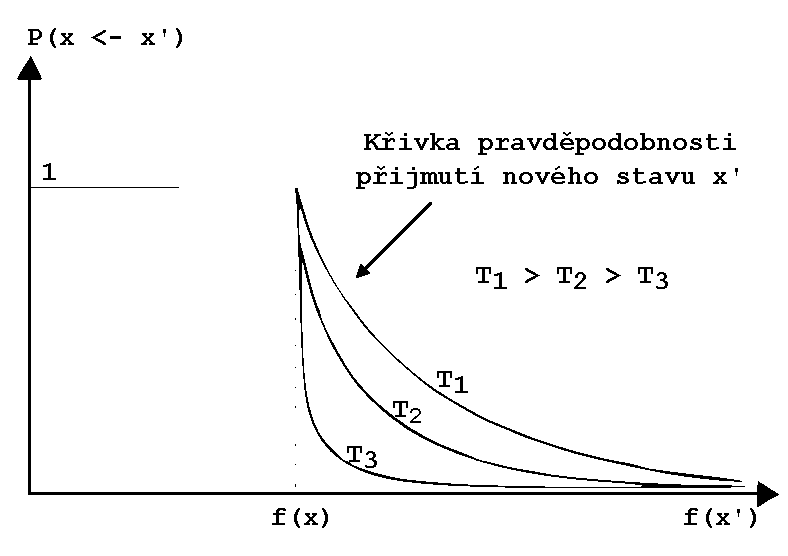
\includegraphics[width=0.5\textwidth]{obrazky-figures/cooling.pdf}
	\caption{Křivka pravděpodobnosti přijetí horšího řešení v~závislosti na teplotě systému. Zdroj: internet.}
	\label{fg:cooling}
\end{figure}

\subsection{Metropolis}
Algoritmus Metropolis~\cite{webMCMC} je MCMC metoda pro získávání náhodných vzorků z~pravděpodobnostní distribuce, u~které je toto vzorkování složité a nebo je distribuční funkce více-dimenzionální. Algoritmus vznikl jako způsob, jak počítačovou simulací zajistit vlastnosti termodynamického systému za pomoci MCMC metody. Pseudokód algoritmu je možné vidět na \ref{code:metropolis}. Algoritmus cyklicky provádí následující:
\begin{itemize}
    \item Vygeneruj kandidátní řešení za pomoci funkce zvané \uv{kernel}. Tato funkce je poskytnuta uživatelem a může být třeba i funkcí generující náhodné čísla. V~případě SA je to funkce \textbf{perturberance} - \ref{eq:perturb} - která je volená tak, aby byla symetrická; pravděpodobnost toho, že malou poruchou se ze stavu A~stane stav B je stejná, jako že ze stavu B se stane stav A. Symetričnost kernel funkce je podmínkou algoritmu Metropolis (ovšem SA funguje i bez splnění tohoto kritéria) 
    
    \item Vygeneruj akceptační kritérium - funkce pravděpodobnosti, která určuje, jak moc se navržené řešení liší od skutečného stavu navrženého Markovským řetězem (stacionární distribuce zmíněná dříve). v~případě SA se jedná o~\textbf{Metropolisovo kritérium}~\ref{eq:metropolisCriter}~\cite{fitWebSA}~\cite{webMCMC}.
    \item Pokud jsou si dostatečně podobné, vygenerovaný stav je přidán do Markovského řetězu~\cite{webMCMC}.
\end{itemize}

\begin{equ}[!ht]
\begin{equation}
\label{eq:perturb}
x_{i+1} = x_i + u~* |x^{max} - x^{min}| * \frac{T}{T^{max}}
\end{equation}
\caption{Funkce perturberance - výběru kandidátního stavu. }
\end{equ}
kde $u$ je náhodné číslo rovnoměrného rozložení mezi $-1$ a $1$, $x_i$ je fitness momentálního stavu, $x^{max}$ a $x^{min}$ jsou fitness hodnoty prozatím nejhoršího a nejlepšího nalezeného stavu resp., $T$ je momentální teplota systému a $T^{max}$ je počáteční teplota.

\begin{equ}[H]
\begin{equation}
\label{eq:metropolisCriter}
\exp(-(\frac{\Delta E}{T_i}))
\end{equation}
\caption{Metropolisovo kritérium pro přijetí horšího stavu v~simulovaném žíhání.}
\end{equ}

\subsection{Rozvrh chlazení}
Většina parametrů simulovaného žíhání - definiční obor, výběr následujícího stavu, atd. - jsou dány již v~definici a za běhu se nemění. O~to více důležitý je pro nalezení optima výběr správného chladícího rozvrhu. Běžně je nejpoužívanější lineární rozvrh chlazení. Ten lze vyjádřit následovně~\cite{Chlebik2017}:

\begin{equ}[H]
\begin{equation}
\label{eq:cooling}
T(i) = T_0 * \alpha^i
\end{equation}
\caption{Běžný lineární rozvrh chlazení systému SA. $(0 \le \alpha \le 1) $}
\end{equ}

Pro vhodně malé $\alpha$, je tento rozvrh dostatečně pomalý a umožní globální konvergenci.

\subsection{Algoritmus}
Pseudokód algoritmu simulovaného žíhaní \cite{Chlebik2017} využívající metodu Metropolis je definován v~algoritmech~\ref{code:SA} a~\ref{code:metropolis}. Je vhodné podotknout, že parametry funkcí například $Perturb$ se považují za proměnné v~globálním prostoru.

\floatname{algorithm}{Algoritmus}
\vspace{\baselineskip}
\begin{algorithm}[H]
\begin{algorithmic}
\State $T := T_{max};$ 
\State $x_{best} := $ náhodně vygenerovaný stav;
 \While{$T > T_{min}$}
 	\State $x_{best} := Metropolis();$
 	\State $T := T * \alpha;$
\EndWhile
\State \Return $x_{best};$
\end{algorithmic}
\caption{Algoritmus simulovaného žíhání}
\label{code:SA}
\end{algorithm}
\begin{algorithm}[H]
\caption{Metropolis}
\label{code:metropolis}
\begin{algorithmic}
  \State $k := 0;$ 
  \State $x_{new} := x_{best};$
 \While{$k < k_{max}$}
 \State $k := k + 1;$
 \State $x_{new} := Perturb();$
 \State $P := \min (1, \frac{exp(-(f(x_{new}) - f(x_{best}))}{T}));$
\If {$random() \leq P$} 
        \State $x := x_{new};$
\EndIf
\EndWhile
\State \Return $x_{new};$
\end{algorithmic}
\end{algorithm}



\section{Tabu prohledávání} %tabu search
\label{algs:ta}
Zakázané prohledávání - častěji v~originálním názvu \uv{Tabu prohledávání} či \uv{Tabu strategie} - je globální optimalizační metoda a meta-heuristika zastřešující rodinu metod, které vnášejí do optimalizačních algoritmů paměťové struktury pro překonání lokálního optima~\cite{Glover2006}. Tabu prohledávání je založeno na premise, že každé řešení problému, které lze klasifikovat jako inteligentní, musí začlenit do svého systému adaptivní paměť, a neslepé, reagující prohledávání. Poté, pokud systém s~pamětí udělá špatnou volbu, je možné se z~této volby díky paměti poučit a upravit strategii. To je v~kontrastu s~návrhem dalších optimalizačních metod založených na přírodních jevech, jakou je například \textit{Simulované žíhání}~\cite{Glover2006}. Tabu prohledávání dostalo své jméno od slova Tabu - \textit{zakázaný} - kvůli své inspiraci v~kulturní evoluci (tabu prohledávání je memotický a evoluční algoritmus). V~kontextu společnosti jsou \uv{tabu} věci taková témata, o~která společnost nestojí a jedinec, který na toto nedbá, bude na nižším společenském postavení a tedy nemusí přežít. 

\subsection{Horolezecká metoda}
\textit{Horolozecký algoritmus}, iterativně prochází stavový prostor. Vždy se z~momentálního stavu rozhlíží po okolí a~pokud je některý z~těchto okolních stavů lepší, přijme jej za současný. Tato logika je opakována po $k$~iterací nebo dokud není dosaženo některé z~ukončovacích podmínek. Takto nejlepší nalezený jedinec je prohlášen za optimum a~algoritmus ukončen. Tato metodika často vede na uváznutí v~oblastech lokálního optima - stav, kdy všechny relativně blízké stavy mají horší fitness. Tento problém je elegantně řešený Tabu strategií zavedením paměti - tzv. Tabu seznamu. Tabu úpravu běžného horolezeckého algoritmu je možné vidět na obrázku~\ref{fg:tabu}.

\begin{figure}[hbt]
	\centering
	\includegraphics[width=0.8\textwidth]{obrazky-figures/tabu.png}
	\caption{Příklad využití strategie Tabu prohledávání nad lokální heuristikou Horolezecké metody (Hill climbing). Bez použití tabu strategie by se Hill climbing dopracoval do stavu $3$, ve kterém by lokálním prohledáním znovuobjevil stav $2$ a přesunul by se do něj.}
	\label{fg:tabu}
\end{figure}

\subsection{Adaptivní paměť}
Na rozdíl od běžných lokálních metod tedy Tabu strategie pracuje se skutečně dynamickým sousedstvím. Tabu prohledávání posouvá lokální heuristiky tak, že upravuje okolí $N(x)$ ($x$ je momentální stav), ze kterého mohou vybírat následující řešení. Toto nové okolí - $N*(x)$ - je omezováno třemi různými typy pamětí~\cite{gloverArt}: 
\begin{itemize}
    \item \textit{krátkodobá paměť} - jednoduchý seznam obsahující $n$ posledně navštívených stavů, kde $n$ je vstupním parametrem algoritmu. Všechny stavy v~tomto seznamu jsou vyloučeny ze sousedství.
    \item \textit{střednědobá paměť} - pravidla, jejichž účelem je vést vyhledávání ke slibným oblastem stavového prostoru. Zde se reálně budou nacházet omezující podmínky specifické pro řešený problém, případně pravidla urychlující konvergenci zakázáním jistých vzorů při vyhledávání.
    \item \textit{dlouhodobá paměť} - pravidla pro udržení diverzity.
\end{itemize}
Rozdíly, mezi těmito druhy pamětí jsou často velice mlhavé a co je pro jeden problém údaj střednědobý, může být v~jiné údajem dlouhodobým nebo naopak. Toto je navíc pouze zjednodušený náhled; koncept těchto pamětí je mnohem složitější a její rozbor pro tuto práci není podstatný. Je pouze vhodné dodat, že adaptivní paměť tabu strategie se dále dělí na nedávnou a opakující  -
\textit{nedávná} ukládá samotné vlastnosti řešení, které se změnily v~nedávné době (jedná se o~jistou úroveň granulity - nezakazujeme celé stavy ale například stavy, jejichž jedna vlastnost je omezena). \textit{Opakující} poté, jak název napovídá, zamezuje cesty, které vedou na cyklus či předčasné konvergenci jedné vlastnosti .
Pro zájemce doporučují například tento článek~\cite{gloverArt} samotného autora algoritmu, ve kterém se této problematice věnuje do hloubky.

\subsection{Algoritmus}
Pseudokód zakázaného prohledávání využívající Horolezeckou metodu je definován v~algoritmu~\ref{code:tabu}. Je vhodné podotknout, že se jedná o~vysokou abstrakci, která prezentuje pouze hlavní smyčku optimalizace a vynechává implementace metod pracujících s~tabu seznamem. $N(x)$ je sousední funkce tak, jak je definována optimalizovaným problémem, $StopCondition()$ je metoda ukončující optimalizace - například dosažením maximálního počtu iterací nebo nalezením optima, pokud je známé.
\begin{algorithm}[H]
\begin{algorithmic}
\State $TabuList := InicializujTabuList();$ 
\State $x_{best}$ := náhodně vygenerovaný stav;
 \While{$! UkoncovaciPodminka()$}
    \State $N^*(x) := Sousedstvi(N(x), TabuList)$
 	\State $x := HillClimbingKrok(x, N^*(x));$
 	\If{$Fitness(x) \leq Fitness(x_{best})$}
 	\State $x_{best} := x$
 	\EndIf
 	\State $AktualizujTabuList(TabuList, x)$
\EndWhile
\State \Return $x_{best};$
\end{algorithmic}
\caption{Strategie Tabu prohledávání využívající Hill-Climbing}
\label{code:tabu}
\end{algorithm}


\section{Diferenciální evoluce}
\label{algs:de}
Diferenciální evoluce, dále DE, je variantou genetického algoritmu specializovaná na problémy řešení spojitých problémů v~reálné doméně (existují ovšem i celočíselné varianty)~\cite{Weisser2010}. Snahou bylo vyvinout robustní, snadno použitelný evoluční algoritmus pro komplexní reálné problémy a to takové u~nichž neznáme přesný předpis účelové funkce~\cite{EVO}. Na rozdíl od ostatních evolučních algoritmů pro řešení úloh v~reálné doméně, se DE vzdává myšlenky, ve které je odvozování nových bodů \uv{slepou funkcí náhody} a namísto ní používá k~odvození informace z~bodů současných. Inspiraci nalézá v~deterministické metodě \textit{Nelder-Mead}.

DE vykazuje následující vlastnosti:
\begin{itemize}
    \item minimální počet řídicích parametrů.
    \item aplikovatelnost na nediferencovatelné funkce.
    \item dobrá a rychlá konvergence.
    \item snadná paralelizace.
\end{itemize}

\subsection{Nelder-Meadův algoritmus}
Jedná se o~známou lokální heuristickou optimalizačních metod pro více-dimenzionální neomezenou optimalizaci bez použití derivací. Myšlenkou metody je obalit stavový prostor do konvexní obálky - simplexu, kterému se postupně za pomocí heuristik budou posouvat body směrem k~optimu. Po dokončení optimalizace bude tento simplex ohraničovat lokální optimum systému. Body simplexu jsou posouvány podle pozice tzv. \textit{centroidu}, což je průměrná hodnota ohodnocení všech bodů simplexu. Dle této hodnoty a pozice nejhoršího bodu se dále vypočítá \textit{reflexní bod}. V~posledním kroku heuristika určí nejvhodnější z~akcí - reflexe, kontrakce, expanze, přiblížení - v~závislosti na fitness hodnotách nových a~dosavadních bodů~\cite{EVO}. Ukázka jednoho stavu a~fungování metody je znázorněn na obrázku~\ref{fg:nm}.

\begin{definition} {Simplex\\}
Simplex \(\mathbb{S} \in \mathbb{R}^n\) je definován jako konvexní obal o~\(n+1\) bodech \(x_0, ..., x_n\) \(x \in \mathbb{R}^n\). Pro \(\mathbb{R}^2\) se jedná o~trojúhelník, pro \(\mathbb{R}^3\) o~čtyřstěn.
\label{def:simplex}
\end{definition}

\begin{figure}[hbt]
	\centering
	\includegraphics[width=0.8\textwidth]{obrazky-figures/nelderMead.png}
	\caption{Ukázka simplexu ve dvourozměrném prostoru a nelder-mead heuristik, které je možné nad tímto simplexem provést. Bod $p_{min}$ může být expandován na bod $p_e$, kontrakcí se z~něj stane centroid - bod $p_c$, reflexí bod $p_r$. Pokud ani jedna z~těchto operací nevylepší fitness hodnotu tohoto bodu v~prostoru, nastane operace přiblížení simplexu. Při této operaci je bod $p_{max}$ posunut na střed jedné ze sousedních hran, podle toho, která je lepším řešením. Body $p_{min}$ a $p_{max}$ označují (při minimalizaci) nejlepší a nejhorší bod v~rámci simplexu.}
	\label{fg:nm}
\end{figure}

\subsection{Řídící parametry a inicializace}
DE pracuje s~populací velikosti $N$, kde chromozom každého jedince je $D$-dimenzionální vektor $x_{i}$, kde $1 \leq i \leq N$ udává číslo jedince v~populaci. Velikost dimenze $D$ je dána dimenzí optimalizovaného problému. Dalšími parametry pro optimální fungování DE je \textit{faktor zesílení} $\beta$ a \textit{pravděpodobnost křížení} $CR$. Špatné zvolení těchto parametrů má detrimentální vliv na schopnost algoritmu nalézt optimum v~rozumném čase~\cite{Weisser2010}.
\begin{itemize}
    \item \textbf{Velikost populace} má přímý vliv na velikost prohledávaného prostoru. S~rostoucí velikostí populace roste pokrytí stavového prostoru, ale také časová složitost algoritmu. Empiricky bylo zjištěno, že velikost populace by měl být přibližně desetinásobek dimenze problému $D$ pro pokrytí celého stavového prostoru. Z~důvodu zrychlení konvergence algoritmu je ovšem častěji použit vztah $N \ge 2n_v + 1$, kde $n_v$ je parametrem selekčního schéma - počet diferenčních vektorů~\cite{Weisser2010}.
    \item \textbf{Faktor zesílení} určuje velikost mutace. Doporučená hodnota je $\beta = 0.5$. Příliš velká hodnota s~sebou přináší riziko přeskočení optima, zatímco příliš malá vede k~pomalé konvergenci a uváznutí. Velikost faktoru zesílení by měla být v~nepřímé úměře k~velikosti populace.
    \item \textbf{Pravděpodobnost křížení} má markantní vliv na diverzitu populace. Při operaci křížení určuje počet parametrů v~rámci jedince, které nebudou zděděny z~rodičovského vektoru. Velká hodnota vede na vysokou diverzitu a snížení schopností lokálního prohledávání prostoru~\cite{Weisser2010}.
    \item \textbf{Strategie} - poslední a velice důležitý parametr, určující jakým způsobem bude vytvářen vektor diferencí a jak bude probíhat křížení. Tato strategie je zapisována ve formátu $DE/x/y/z$, a platí že $x$ označuje způsob výběru bázového vektoru, $y$ počet vektorů pro výpočet vektoru diferencí a $z$ je typ křížení. Mezi nejpoužívanější (ovšem zdaleka ne jediné) strategie patří $DE/rand/1/bin$ nebo $DE/best/2/bin$~\cite{EVO}. Každá ze strategií s~sebou přináší výhody a nevýhody a jejich studium přesahuje rámec této práce. Pro zájemce doporučuji tento článek~\cite{DE_MUTATIONS}, který se této problematice věnuje.
\end{itemize}

Inicializace počáteční populace probíhá náhodně, pro každý parametr vždy v~rozmezí jeho definičního oboru.

\subsection{Mutace}
Mutace je v~kontextu DE chápána jako vytvoření tzv. vektoru diferencí (v~literatuře také šumový vektor) $\Vec{v_i}$, a je to základní stavební kámen celého algoritmu. Tento vektor slouží při křížení jako druhý rodič a způsob jeho vzniku je určen dříve zmíněným parametrem DE - strategie. Následující příklad popisuje vytvoření vektoru diferencí několika běžnými strategiemi~\cite{DE_IEEE, Weisser2010}. Parametr typu křížení nemá na generování mutací vliv a proto je zde vynechán.

\begin{itemize}
    \item \textbf{DE/rand/1} - šumový vektor je počítán ze tří náhodně vybraných jedinců z~aktuální populace. Váhovaný rozdíl (diference) mezi dvěma náhodně vybranými jedinci $\Vec{x_{r_2}}$ a $\Vec{x_{r_3}}$
    je připočten ke třetímu náhodnému jedinci $\Vec{x_{r_1}}$. Platí, že $r_1 \neq r_2 \neq r_3$. Graficky zobrazeno na obrázku~\ref{fg:de}. Rovnice tohoto vztahu:
    \begin{equation}
    \Vec{v_i} = \Vec{x_{r_1}} + \beta * (\Vec{x_{r_2}} - \Vec{x_{r_3}})
    \label{eq:de_rand_1}
    \end{equation} 

    \item \textbf{DE/rand/2} - modifikace $DE/rand/1/$. Vektor je počítán ze $4$ náhodných unikátních jedinců:
        \begin{equation}
    \Vec{v_i} = \Vec{x_{r_1}} + \beta * (\Vec{x_{r_2}} +\Vec{x_{r_3}} - \Vec{x_{r_4}} - \Vec{x_{r_5}})
    \label{eq:de_rand_2}
    \end{equation} 
    
    \item \textbf{DE/best/1} - je podobný $DE/rand/1/$; liší se pouze ve vektoru, ke kterému je připočítáván výsledek. V~této strategii se jedná o~$x_{best}$, tedy doposud nejlepší nalezený jedinec.
    \begin{equation}
    \Vec{v_i} = \Vec{x_{best}} + \beta * (\Vec{x_{r_2}} - \Vec{x_{r_3}})
    \label{eq:de_rand_1}
    \end{equation} 

    \item \textbf{DE/best/2} - analogicky k~$DE/rand/1$ a $DE/best/1$ vznikl $DE/best/2$ modifikací $DE/rand/2$.
    \begin{equation}
    \Vec{v_i} = \Vec{x_{best}} + \beta * (\Vec{x_{r_2}} +\Vec{x_{r_3}} - \Vec{x_{r_4}} - \Vec{x_{r_5}})
    \label{eq:de_rand_2}
    \end{equation} 
\end{itemize}

\noindent Jak je vidět, ve skutečnosti nic nebrání použití více než jednoho páru vektorů pro lineární kombinaci. Obecný tvar takové kombinace lze vyjádřit takto : 
 \begin{equation}
    \Vec{v_i} = \Vec{x_0} + \beta * \sum_{n=1}^{n_v}(\Vec{x_{r_{1}^{n}}} - \Vec{x_{r_{2}^{n}}})
    \label{eq:de_rand_2}
    \end{equation} 
kde $n_v$ bude počet dvojic vektorů, které si přejeme kombinovat a $x_0$ bude nějaký bázový vektor, který se liší od ostatních - nejlepší v~$best$ strategiích, náhodný v~$rand$~\cite{Weisser2010}.

Další známe strategie jsou~\cite{Weisser2010}:
\begin{itemize}
    \item \textbf{DE/current-to-best/$n_{v}$}, které pracuje s~momentálním řešením $i$ jako bázovým, ke kterému je připočítána váhovaná vzdálenost od nejlepšího $best$ spolu s~váhovanou vzdáleností dalších $n_v$ párů dvou náhodných unikátních $r_1$ a $r_2$.
     \begin{equation}
    \Vec{v_i} = \Vec{x_i} +  \beta * (\Vec{x_{best}} - \Vec{x_{i}}) + \beta * \sum_{n=1}^{n_v}(\Vec{x_{r_{1}^{n}}} - \Vec{x_{r_{2}^{n}}})
    \label{eq:de_rand_2}
    \end{equation} 
    \item \textbf{DE/rand-to-best/$n_{v}$}, které kombinuje přístup strategií $rand$ a $best$ - bázový vektor je poměr nejlepšího a náhodně vybraného vektoru udávaný náhodným parametrem $\gamma$.
     \begin{equation}
    \Vec{v_i} = \gamma * \Vec{x_{best}} + (1 - \gamma) * \Vec{x_{r_1}}  + \beta * \sum_{n=1}^{n_v}(\Vec{x_{r_{2}^{n}}} - \Vec{x_{r_{3}^{n}}})
    \label{eq:de_rand_2}
    \end{equation} 
    Opět zde platí, že náhodně generované vektory musí být unikátní a $0 \leq \gamma \leq 1$.
\end{itemize}


\subsection{Křížení a selekce}
Operace křížení následuje po vytvoření vektoru diferencí. Slouží k~vygenerování potomka - tzv. \textit{zkušebního vektoru} $x_{new}$~\cite{Weisser2010}. Ten je vytvořen za pomoci následujícího vztahu: 
     \begin{equation}
    \Vec{x_{new}}[k] = \begin{cases}
    \Vec{v_{i}}[k] & \text{ $N(0,1) \le CR$}\\
    \Vec{x_{i}}[k] &\text{jinak}
    \end{cases}
    \label{eq:de_rand_2}
    \end{equation} 
kde $\Vec{x_i[k]}$ je gen $k$ rodiče $\Vec{x_i}$, $\Vec{v_i[k]}$ je gen $k$ vektoru diferencí $\Vec{v_i}$ a $N(0,1)$ je náhodně vygenerované číslo od $0$ do $1$ normálním pravděpodobnostním rozložením.

Do nové populace je poté vybrán ten jedinec, který má lepší výsledky účelové funkce.

\begin{figure}[hbt]
	\centering
	\includegraphics[width=0.8\textwidth]{obrazky-figures/de.pdf}
	\caption{Ukázka generování vektoru diferencí $v_i$ ve 2D prostoru strategií $DE/rand/1$. Převzato z~\cite{EVO}.}
	\label{fg:de}
\end{figure}

\section{Optimalizace hejnem částic}
\label{algs:pso}
Optimalizace hejnem částic~\cite{EVO}, anglicky Particle Swarm Optimization - PSO, je evoluční optimalizační technika inspirovaná pohybem zvířat v~hejnech, zejména ptáků. Bylo zjištěno, že schopnosti kolektivní spolupráce jedinců při vykonávaných činnostech (například hledání potravy) poskytuje těmto druhům evoluční výhodu. Metoda patří do skupiny zvané částicové systémy a od svého vzniku v~roce 1995 se pro tuto skupinu stala, společně s~metodou optimalizace mravenčí kolonií (ACO), hlavním představitelem. Na rozdíl od ACO, které je vhodnější spíše pro problémy diskrétního charakteru, je PSO navrženo pro problémy definované na spojité doméně. 

V~algoritmu je počet jednoduchých agentů - částic - umístěn do stavového prostoru optimalizovaného problému a každému z~nich je spočtena jeho fitness hodnota. Každý z~agentů poté spočítá svůj následující pohyb tak, že vezme v~potaz historii jeho vlastního pohybu, historii pohybu zbytku agentů v~hejnu a přidáním náhodné odchylky. Další iterace nastane poté, co se všechny částice pohnou na své nové pozice. Nakonec celé hejno, stejně jako hejno ptáků společně hledající jídlo, konverguje k~optimu~\cite{pso_article}. Princip zobrazen na obrázku~\ref{fg:pso_swarm}. 

Samotná částice by nebyla schopná nalézt optimum, jedná se o~emergentní vlastnost začlenění částic do společnosti a komunikovat. Tato společnost nemá vůdce ani žádnou centrální inteligence, přesto je schopna býti více než pouze součtem svých prvků.

\begin{definition} {Emergence\\}
Spontánní vznik makroskopických vlastností a struktur složitých systémů, jež není snadné odvodit z~vlastních jejich složek.
\label{def:emergence}
\end{definition}

\begin{figure}[hbt]
	\centering
	\includegraphics[width=0.8\textwidth]{obrazky-figures/pso.png}
	\caption{Vizualizace stavového prostoru s~částicemi na začátku (vlevo) a konci (vpravo) vykonávání PSO. Zdroj: internet.}
	\label{fg:pso_swarm}
\end{figure}

\subsection{Částice}
Každá částice v~hejnu se skládá ze tří D-dimenzionálních vektorů, kde $D$ je dimenze prohledávaného problému~\cite{pso_article}.
\begin{itemize}
    \item \textbf{Momentální pozice} \textbf{$\Vec{x}$.}
    \item \textbf{Dosavadní nejlepší pozice.} \textbf{$\Vec{p}$.}
    \item \textbf{Rychlost a směr pohybu.} \textbf{$\Vec{v}$.}
\end{itemize}
Momentální pozice je inicializována náhodnou hodnotou v~rámci stavového prostoru, dosavadní nejlepší pozice na zástupnou hodnotu, jejíž hodnota musí být horší než hodnota libovolného stavu ve stavovém prostoru. Rychlost a směr je inicializován náhodně ovšem v~rozumném rozmezí.


\subsection{Topologie}
Aby byla možná komunikace mezi jedinci, populace je uspořádána do jisté topologie~\cite{pso_article} - sociální sítě. Tuto síť si lze představit jako propojení dvou částic neorientovanou hranou, celou topologii si je poté možné představit jako neorientovaný graf. Částice má poté své \textit{sousedy}, kteří vytváří její \textit{sousedství} (nejedná se o~tranzitivní relaci). Toto rozdělení je důležité - částice ve stejném sousedství tíhnou k~prohledávání stejné oblasti. Každá částice objeví svou část prostoru a informuje o~tom sousedy. Ostatní částice o~této oblasti dostanou informaci až od svých sousedů - informační zpoždění. 

Originální PSO využívalo Euklidovského sousedství. To se ovšem prokázalo jako výpočetně náročná topologie s~nevhodnými konvergenčními vlastnostmi~\cite{pso_article}. V~současné době nejpoužívanější topologie jsou založeny na sociálním sousedství. Jedinci jsou sousedy bez ohledu na to, ve které části stavového prostoru se zrovna nacházejí. 

Typ sousedství se obecně rozděluje na dva druhy~\cite{pso_article}:

\begin{itemize}
    \item \textbf{Statická sousedství} - jak název napovídá, jedná se o~sousedství která se nemění v~průběhu vykonávání algoritmu. Typickým příkladem takového sousedství je tzv. \textit{gbest} -  úplná - topologie (obrázek~\ref{fg:pso_swarmTopo}). Dalším je \textit{lbest} topologie - kruh. Toto sousedství dovoluje paralelní prohledávání - rozdělení na regiony podle sousedství. Tato topologie konverguje pomaleji než gbest, ovšem lépe dokáže rozpoznat lokální optima a vyhnout se jim. Kompromisem mezi těmito topologiemi je \textit{von Neumann}, který dokáže kombinovat výhody obou. Obecně platí, že pro unimodální problémy jsou vhodnější gbest topologie, zatímco pro multimodální lbest.
    \item \textbf{Dynamická sousedství} - topologie měnící počet sousedů i sousedy samotné v~průběhu vykonávání algoritmu. Například uveďme techniku, při které se začíná s~lbest topologie pro podporu prohledávání a postupem času se přelíná do gbest pro podporu exploitace.
\end{itemize}


\begin{figure}[H]
	\centering
	\includegraphics[width=0.6\textwidth]{obrazky-figures/psoTopo.jpg}
	\caption{Nejznámější PSO topologie.}
	\label{fg:pso_swarmTopo}
\end{figure}


\subsection{Výpočet směru}
 Nová pozice jedince je v~kanonickém PSO udána následující rovnicí~\cite{pso_article} (grafické znázornění je na obrázku~\ref{fg:pso_swarmProc}): 
    \begin{equation}
    \Vec{x_{i}}(g+1) = \Vec{x_{i}}(g) + \Vec{v_{i}}(g+1)
    \label{eq:pso1}
    \end{equation} 
kde $i$ udává jedince v~populaci, $\Vec{x_i}$ jeho pozici a $\Vec{v_i}$ jeho rychlost; $g$ je současná generace. Výpočet $\Vec{v_i}$ pro gen $j$ v~generaci $g$:

    \begin{equation}
    \Vec{v_{i}}[j](g+1) = \Vec{v_{i}}[j](g) + C_1 + C_2
        \label{eq:pso2}
    \end{equation} 
    
    \begin{equation}
     C_1 = c_1*N(0,1)* ( pBest_i[j](g) - \Vec{x_{i}}[j](g))
    \label{eq:pso3}
    \end{equation} 
    
    \begin{equation}
     C_2 = c_2*N(0,1)* ( gBest[j](g) - \Vec{x_{i}}[j](g))
    \label{eq:pso3}
    \end{equation} 
    

\begin{itemize}
    \item $pBest_i[j](g)$ je nejlepší nalezená pozice jedince $i$ pro gen $j$ v~generaci $g$.
    \item $gBest[j](g)$ je nejlepší nalezená pozice v~celém sousedství pro gen $j$ v~generaci $g$.
    \item $c_1$ a $c_2$ - akcelerační koeficienty.
    \item $N(0,1)$ - náhodně vygenerované číslo od $0$ do $1$ normálním pravděpodobnostním rozložením.
\end{itemize}


\begin{figure}[hbt]
	\centering
	\includegraphics[width=0.8\textwidth]{obrazky-figures/pso2.pdf}
	\caption{Proces výpočtu následujícího směru pohybu částice. Dosavadní směr pohybu částice je přebit směrem pohybu hejna. Zdroj:~\cite{webPSO}.}
	\label{fg:pso_swarmProc}
\end{figure}



\subsection{Parametry}
PSO vyžaduje pro správné fungování nastavení při nejmenším následujících parametrů:

\subsubsection{Akcelerační koeficienty}
Koeficienty $c_1$ a $c_2$ určují, jak velkou váhu dává algoritmus nejlepším nalezeným pozicím agentem samotným ($pBest$ - $c_1$) a v~rámci sousedství ($gBest$ - $c_2$). Špatně nastavené koeficienty naruší rovnováhu prohledávání a vykořisťování a neumožní algoritmu konvergovat ke globálnímu optimu. Obecně se nastavuje $c_1 = c_2 = 2$ - částice přeletí optimum v~polovině případů. Čím vyšší je součet koeficientů, tím stoupá četnost oscilací kolem optima~\cite{pso_article}.

\subsubsection{Počet částic}
Vysoce závislé na typu problému, ovšem obecně se udává mezi 20 - 50 částicemi.

\subsubsection{Maximální rychlost částice}
Částicím je třeba omezit rychlost; při příliš velkých rychlostech by se mohlo stát, že částice bude provádět příliš velké kroky a optimum přeskakovat. Proto byla zaveden parametr $V_{max}$ a $V_{min}$, tedy minimální a maximální rychlost, kterou se může částice pohybovat. Dále se doporučuje, aby $V_{min} = - V_{max}$. V~případě, že částice povolenou rychlost překročí, je zastavena a je jí vygenerována nová náhodná rychlost ve stejném směru. I~zde je volba těchto parametrů závislá na problému, příliš nízká maximální rychlost omezuje prohledávání, zatímco příliš vysoká vykořisťování.



\subsection{Algoritmus}
Pseudokód algoritmu PSO vypadá následovně:

\begin{algorithm}[H]
\begin{algorithmic}
\State $InicializujHejnoCastic();$
\While{$! UkoncovaciPodminka()$}
\ForAll{$p \in Hejno$}
    \State $x = Pozice(p)$;
    \If{$Fitness(x) \leq Fitness(pBest(p)) $}
 	    \State $pBestUpdate(p, x)$
 	\EndIf
\EndFor
\State $gBestUpdate(pBest, Hejno)$
\ForAll{$p \in Hejno$}
     \State $VypocitejRychlostCastice(p)$
     \State $VypocitejPoziciCastice(p)$
\EndFor
\EndWhile
\State \Return $gBest;$
\end{algorithmic}
\caption{Optimalize hejnem částic}
\label{code:tabu}
\end{algorithm}

%%%%%%%%%%%%%%%%%%%%%%%%%%%%%%%%%%%%%%%%%%%%%%%%
\section{Evoluční strategie založená na adaptaci kovarianční \\\mbox{matice}}
\label{algs:cmaes}
Metoda známá pod zkratkou \uv{CMA-ES}, z~anglického \uv{Covariance Matrix Adaptation - Evolution Strategy}~\cite{CMAES}, je moderní state-of-the-art metoda pro optimalizaci v~doméně reálných čísel. Stejně jako ostatní EA, i ze je využíváno stochastických prvků. Základní kanonická verze \textit{evoluční strategie} využívá jako svůj hnací motor mutaci svých jedinců o~náhodnou hodnotu z~rozložení s~pevně danou směrodatnou odchylku $\sigma$. CMA-ES tento princip rozšiřuje použitím tzv. kovarianční matice, na základě které generuje nové jedince. Tato matice je neustále adaptována podle dosavadního stavu populace a umožňuje tak dynamicky upravovat velikost kroku a tím i prohledávaný stavový prostor. Tato adaptace poté udává tzv. cestu evoluce, kterou algoritmus používá k~učení a stanovení následujícího kroku směrem k~optimu. Algoritmus samotný nevyžaduje hluboké nastavování řídicích parametrů, což může být výhodou.

\subsection{Kovariance}
\label{ss:kovar}
Statistická charakteristika, určující míru lineární závislosti náhodných veličin $X$ a $Y$.
$$c(X,Y) = E[(X-E[X])*(Y-E[Y])]$$
kde $E[X]$ je střední hodnotou náhodné veličiny $X$.
\begin{itemize}
    \item $c(X,Y) > 0$ - veličiny se pohybují stejným směrem.
    \item $c(X,Y) < 0$ - veličiny se pohybují opačným směrem.
    \item $c(X,Y) = 0$ - veličiny jsou nezávislé.
\end{itemize}
Kovarianční matice $C$ pro $N$ proměnných je poté $N \times N$ matice, jejíž prvky jsou kovariance mezi proměnnými ($C_{ij}$ je spočtena jako $c(I,J)$). Na diagonále této matice je poté standardní odchylka náhodné veličiny $I$~\cite{CMAES}. Obecně lze vytvořit kovarianční matici pro libovolnou distribuční funkci, nejčastěji (jako i v~CMA-ES) se setkáme s~rozložením normálním.

\subsection{Adaptace}
Adaptace matice kovariancí zhruba odpovídá tzv. rekurzivní \textit{rank update} funkci. Jedná se o~přibližný, ovšem při vhodné volbě parametrů, dostatečně přesný odhad, abychom mohli považovat každou iteraci kovarianční matice za validní. Bylo zjištěno, že rank-one metoda je nejlepším estimátorem pro velké populace (obecně $\lambda/4 > 1 + \log n$)~\cite{CMAES}.

\subsubsection{Rank-One Update}
Základní operace nad maticí, odpovídající transformaci~\ref{eq:rankOneUpdate}. 
\begin{equation}
    A~+ \Vec{u}*\Vec{v}^T
    \label{eq:rankOneUpdate}
\end{equation}
kde $A$ je $K \times K$ matice a $u$ a $v$ dva $K \times 1$ vektory. Rank-One dostal svůj název kvůli hodnosti matice vzniklé vynásobením vektorů (matice hodnosti $1$).

Při adaptaci vypadá rank-one update následovně~\cite{CMAES}. Začínáme s~$m \in \mathbb{R}^n$, $C = \textbf{I}$, $\sigma = 1$, rychlost učení $c_{cov} \approx \frac{2}{n^2}$, $w_i$ je váha, která náleží vektoru $\Vec{y_i}$. Platí, že $\sum_{i=1}^{\mu}w_i = 1 $ a zároveň je $w_{i=1 \dots \lambda}$ nastaveno tak, aby platilo, že~\ref{eq:cmaes_muWeights} $\approx 0.4\lambda$. 
    \begin{subequations}
    \label{eq:cmaes}
    \begin{align}
        \Vec{x_i} &= \Vec{m} + \Vec{\sigma} \Vec{y_i}, \qquad \Vec{y_i} \sim N_i(\Vec{0}, C)  \label{eq:cmaes_sampling}\\
        \Vec{m} &\leftarrow \Vec{m} + \Vec{\sigma} \Vec{y_w}, \qquad \Vec{y_w} = \sum_{i=1}^{\mu}w_i\Vec{y_i} \label{eq:cmaes_mean}\\ 
        C &\leftarrow (1 - c_{cov})*C + c_{cov}* \mu_{w} * \underbrace{\Vec{y_{w}}\Vec{y_{w}}^{T}}_\text{rank-one}  \label{eq:cmaes_cUpdate} \\
        \mu_{w} &= \frac{1}{\sum_{i=0}^{\mu}w_{i}^{2}} \approx 0.4\lambda \label{eq:cmaes_muWeights} 
    \end{align}
    \label{eq:rankOne1}
    \end{subequations} 

V~těchto rovnicích je skryt téměř celý algoritmus CMA-ES. Zjednodušeně:
\begin{itemize}
    \item Je provedeno ohodnocení všech jedinců v~populaci, rovnice~\ref{eq:cmaes_sampling}.
    \item Je vybráno $\mu$ jedinců, jejichž váhová suma, společně se standardní odchylkou posouvá nový průměr příští generace. Přiřazování vah si lze představit jako selekční mechanismus tohoto algoritmu. Je nutno zmínit, že \textbf{je vybráno $\mu$ nejlepších řešení} (získáno fitness ohodnocením $\Vec{x_i}$), nikoliv náhodných. Rovnice~\ref{eq:cmaes_mean}.
    \item Za pomoci zmíněné sumy je adaptována kovarianční matice $C$.  Rovnice~\ref{eq:cmaes_cUpdate}.
\end{itemize}
\\
Adaptace matice způsobí, že CMA-ES~\cite{CMAES}
\begin{itemize}
    \item postupně zjistí všechny párové závislosti mezi proměnnými.
    \item provede analýzu hlavních komponent kroků $y_w$ tak, jak šli za sebou - rozložení na charakteristické vektory lineárních transformací kovarianční matice (rank update matice je symetrická, což zaručuje rozklad) - umožní rozpoznat libovolnou rotaci stavového prostoru proměnných a řešit takto rotovaný problém.
\end{itemize}
\\
a pokud je $\mu = 1$ poté je pro průměr nové generace vždy vybrán nejlepší jedinec v~populaci a CMA-ES provádí populační hill-climbing algoritus nad distribucí proměnných $N$.

Toto je v~krocích téměř celý algoritmus CMA-ES. Zásadní rozdíl mezi rovnicemi~\ref{eq:cmaes} a skutečným algoritmem je v~samotné adaptaci matice $C$. Pro její aktualizaci je ve skutečnosti vypočtena \emph{evoluční cesta}. Dále je třeba dát CMA-ES dříve zmíněnou dynamičnost postupnou úpravou standardní odchylky $\sigma$.

\subsubsection{Evoluční cesta}
Konceptuálně se jedná o~cestu, kterou se strategie vydala při hledání řešení. Znázorněno na obrázku~\ref{fg:evoPath}. Rekonstrukce této cesty se nazývá \textbf{kumulací} (nebo také například \uv{momentum} při fázi zpětné propagace umělých neuronových sítích - učení). Kumulace je v~CMA-ES spočtena dvakrát, tzv. \textbf{\uv{isotropická}}~\ref{eq:cmaes_po}, pro adaptaci zmíněné odchylky a~tím velikosti kroku algoritmu; a poté cesta \textbf{\uv{anisotropická}}~\ref{eq:cmaes_pc}. Tato cesta slouží k~adaptaci kovarianční matice a~směru, kterým se algoritmus vydá při zkoumání stavového prostoru~\cite{CMAES}. 


\begin{figure}[hbt]
	\centering
	\includegraphics[width=0.65\textwidth]{obrazky-figures/evoPath.pdf}
	\caption{Názorná ukázka evoluční cesty. Elipsoidy znázorňují distribuční rozsah, tvar i střed je udán kovarianční maticí v~odpovídajícím kroku evoluce.}
	\label{fg:evoPath}
\end{figure}

Nechť $k$ označuje generaci
    \begin{subequations}
    \label{eq:cmaes}
    \begin{align}
        \Vec{p_\sigma}^{(k+1)} &\leftarrow (1 - c_{\sigma})\Vec{p_\sigma}^{k} + \sqrt{1 - (1 - c_{\sigma})^2} \sqrt{\mu_{w}}C^{-\frac{1}{2}}\Vec{y_w} \label{eq:cmaes_po}\\
        \Vec{p_c}^{(k+1)} &\leftarrow (1 - c_{c})\Vec{p_c}^{k} + h_{\sigma}*\sqrt{1 - (1 - c_{c})^2} \sqrt{\mu_{w}}\Vec{y_w} \label{eq:cmaes_pc}\\
        \mu_{w} &= \frac{1}{\sum_{i=0}^{\mu}w_{i}^{2}}, c_{cov} \ll c_c \approx c_{\sigma} \ll 1 \\
        h_{\sigma} &= 
        \begin{cases} 
            1       & pokud \quad \| p_{\sigma}\| < 1.5\sqrt{n}\\
            0       & jinak
        \end{cases}
    \end{align}
    \label{eq:pc}
    \end{subequations} 
\begin{itemize}
    \item $c_{c}$ a $c_{\sigma}$ jsou učící faktory pro anisotropickou a isotropickou cestu resp. Bylo ovšem zjištěno, že tyto hodnoty iterativně degradovaly přirozený rozptyl proměnných. Z~tohoto důvodu byly přidány normalizační výrazy (odmocnina $\sqrt{1-(1-c_{x})^2}$), které tento efekt zastavují (nastavením hodnot na 1 se z~rovnic vytratí i zmíněné mocniny).
    \item $C^{-\frac{1}{2}}$ - symmetrická odmocnina z~matice preciznosti (inverze kovarianční matice - obecně udává, jak moc je třeba transformovat originální data, aby byla nezávislá).
    \item $h_{\sigma}$ je zdržovací funkce. V~případě, že $\| p_{\sigma}\|$ je příliš vysoké, by docházelo k~příliš rychlému růstu elipsoidu daného maticí $C$ a tím i nechtěné diverzifikaci populace.
\end{itemize}


\subsubsection{Rank-$\mu$ update}
Pokud problém vyžaduje rychlou konvergenci (i za cenu globálního prohledávání), je třeba volit menší velikost populace. V~takovém případě ovšem již estimátor rank-one update není validní a je třeba využít jiné metodiky. Zde přichází na řadu \uv{Rank-$\mu$}. K~výpočtu následující kovariance je použita informace z~celé generace, na rozdíl od informace o~korelacích mezi generacemi.
\begin{subequation}
    \label{eq:rankMuC}
    \begin{align}
        C^{(k+1)} &= (1-c_{\mu}\sum w_i)C^k + c_{\mu}\sum_{i=1}^{\lambda}w_i \Vec{z_{i}}^{(k+1)}({\Vec{z_{i}}^{(k+1)}})^T \\
        z_{i}^{(k+1)} &= \frac{(y_{i}^{(k+1)} - m^k)}{\sigma_{i}^{k}}
    \end{align}
\end{subequation}

\subsection{Konečná podoba rovnic}
Kombinací rank-one a rank-$\mu$ metodik vzniká výsledná podoba adaptace kovarianční matice:
\begin{subequation}
    \label{eq:cmaes_rankMuC}
    \begin{align}
        C^{(k+1)} &\leftarrow (1-c_{cov}-c_{\mu}\sum w_i)C^k \nonumber \\ 
                &+ \underbrace{c_{cov}*\Vec{p_c}^{(k+1)}(\Vec{p_c}^{(k+1)})^T }_\text{rank-one} + \underbrace{c_{\mu}\sum_{i=1}^{\lambda}w_i \Vec{z_{i}}^{(k+1)}({\Vec{z_{i}}^{(k+1)}})^T}_\text{rank-$\mu$}
    \end{align}
\end{subequation}


\pagebreak
\noindent Přidáme-li i rovnici adaptace velikosti kroku $\sigma$, získáváme kompletní algoritmus \emph{CMA-ES}:

\begin{subequation}
\begin{gathered}
    \Vec{x_i} \leftarrow \Vec{m} + \Vec{\sigma} \Vec{y_i}, \qquad \Vec{y_i} \sim N_i(\Vec{0}, C)\vspace{4mm}\\
    sort(\Vec{y_i})\text{ podle hodnoty }f(\Vec{x_i})\\
    \Vec{m} \leftarrow \Vec{m} + \Vec{\sigma} \Vec{y_w}, \qquad \Vec{y_w} \leftarrow \sum_{i=1}^{\mu}w_i\Vec{y_i}\\ 
    \Vec{p_\sigma}^{(k+1)} \leftarrow (1 - c_{\sigma})\Vec{p_\sigma}^{k} + \sqrt{1 - (1 - c_{\sigma})^2} \sqrt{\mu_{w}}C^{-\frac{1}{2}}\Vec{y_w}\\
    \\
    \Vec{p_c}^{(k+1)} \leftarrow (1 - c_{c})\Vec{p_c}^{k} + h_{\sigma}*\sqrt{1 - (1 - c_{c})^2} \sqrt{\mu_{w}}\Vec{y_w}\\
    \\
    \mu_{w} \leftarrow \frac{1}{\sum_{i=0}^{\mu}w_{i}^{2}} \quad  h_{\sigma} \leftarrow 
        \begin{cases} 
            1       & \text{pokud} \quad \| p_{\sigma}\| < 1.5\sqrt{n}\\
            0       & \text{jinak}
        \end{cases}\\
        \\
        z_{i}^{(k+1)} = \frac{(y_{i}^{(k+1)} - m^k)}{\sigma_{i}^{k}}
        \\
        C^{(k+1)} \leftarrow (1-c_{cov}-c_{\mu}\sum w_i)*C^k \nonumber  + \underbrace{c_{cov}*\Vec{p_c}^{(k+1)}(\Vec{p_c}^{(k+1)})^T }_\text{rank-one} + \underbrace{c_{\mu}\sum_{i=1}^{\lambda}w_i \Vec{z_{i}}^{(k+1)}({\Vec{z_{i}}^{(k+1)}})^T}_\text{rank-$\mu$}\\
        \\
     \Vec{\sigma}^{(k+1)} \leftarrow  \Vec{\sigma}^{k} * \exp{\left(    \frac{c_{\sigma}}{1+\sqrt{\frac{\mu_w}{n}}}*\left[\frac{\|p_{\sigma}\|}{E\|N(\Vec{0}, \textbf{I})\|} - 1\right]\right)}
\end{gathered}
\end{subequation}
\\\\\\
\\
\\
\noindent
\begin{minipage}[t]{.33\textwidth}
Empiricky bylo zjištěno:
\begin{itemize}
    \item $\lambda \approx 4 + 3* \log N$ 
    \item $\mu \approx \frac{\lambda}{4}$
    \item $c_{cov} \approx \frac{2}{n^2}$
    \item $c_c \approx c_{\sigma} \approx \frac{4}{n}$
    \item $c_{\mu} \approx \min(\frac{\mu_w}{n^2}, 1-c_{cov})$
    \item $c_{cov} + c_{\mu} \le 1$
    \item $\sum w_i=\sum_{j=1}^{\lambda}w_j\approx\frac{-c_{cov}}{c_{\mu}}$
\end{itemize}
\end{minipage}
\hfill
\noindent
\begin{minipage}[t]{.32\textwidth}

Iniciální hodnoty:
\begin{itemize}
    \item $C = \textbf{I}$ 
    \item $p_c = \Vec{0}$
    \item $p_{\sigma} = \Vec{0}$
\end{itemize}
\end{minipage}
\begin{minipage}[t]{.32\textwidth}

Vstupy:
\begin{itemize}
    
    \item $\Vec{m} \in \mathbb{R}^n$ - počáteční průměrná hodnota 
    \item $\Vec{\sigma} \in \mathbb{R}_+$ - počáteční standardní odchylky jednotlivých proměnných
    \item $k_{max}$ - maximální počet generací
\end{itemize}
\end{minipage}

\chapter{Implementace a testování}
\label{impl}
Následující kapitola si nejprve klade za cíl představit vytvořený programový základ, který byl použit pro řešení problému hledání trajektorie sonikací. Následně představí několik běžných matematických funkcí pro testování optimalizačních metod, na kterých bude ověřena optimalizační schopnost vytvořeného řešení. Funkce nebyly vybrány náhodně, každá z~nich má odlišné vlastnosti a~testuje algoritmy podle jiných kritérií. V~poslední části budou prezentovány výsledky testovacích běhu, vedeny úvahy nad těmito výsledky a diskutována schopnost optimalizovat trajektorii sonikací \emph{HIFU}.
\section{Implementace}
Každý z~algoritmů představených v~kapitole~\ref{algs} byl implementován jako spustitelný optimalizér v~jazyce \emph{C++11} za pomoci externích knihoven \emph{GAUL}\footnote{\url{http://gaul.sourceforge.net/}} pro metody \emph{Genetického algoritmu}, \emph{Simulovaného žíhání}, \emph{Tabu prohledávání} a \emph{Diferenciální evoluce}, \emph{LibOPT}\footnote{\url{https://github.com/jppbsi/LibOPT}} pro metodu \emph{Optimalizace rojem částic} a \emph{CMA-ESpp}\footnote{\url{https://github.com/AlexanderFabisch/CMA-ESpp}} pro metodu \emph{CMA-ES}. Všechny tyto knihovny byly v~malé míře upraveny od jejich běžně dostupné varianty pro potřeby této práce. 

Dále vzniklo několik skriptů v~prostředí \emph{Bash} pro paralelní spuštění a sběr výsledků nezávislých optimalizací na clusterech \emph{IT4Innovation}. Skript v~jazyce \emph{Python3} pro generování relevantních statistických grafů z~těchto výsledků za pomoci balíčku \emph{MatplotLib}\footnote{\url{https://matplotlib.org/index.html}}. Pro překlad je poskytnut vzorový \texttt{Makefile} soubor. 

Implementované optimalizační programy a skripty pro kolekci dat vznikly pouze jako nezbytný nástroj pro potřeby této práce. Pro úpravy se předpokládá znalost programování, optimalizačních metod a alespoň mírná znalost rozhraní a datových struktur použitých externích knihoven. Všechen kód je řádně dokumentován v~doxygen komentářích ve zdrojových souborech.

\subsection{Sjednocení rozhraní externích knihoven}
Každá z~optimalizačních knihoven má výrazně odlišné rozhraní spuštění. Nastavení fitness funkce, podmínky konvergence a přerušení. I~výstupního protokol průběhových dat procesu optimalizace se výrazně liší. Z~toho důvodu bylo třeba vytvořit novou vrstvu mezi uživatelem a začátkem procesu optimalizace. Pro snadnou úpravu a jednotné spuštění procesu byl vytvořen modulární návrh využívající jednotných deklarací rozhraní v~hlavičkovém souboru. Tyto funkce jsou poté zakomponovány v~rámci unifikované mezivrstvy mezi spouštěnou aplikací a funkcí optimalizace externí knihovny. Samotná implementace metod je optimalizačnímu programu poskytnuta při linkovacím procesu v~průběhu překladu. Implementace nové fitness funkce je tedy možná definicí funkcí z~jednotného hlavičkového souboru a následné přilinkování tohoto souboru při překladu. Je nutné podotknout, že vzniklé optimalizační programy minimalizují.

\subsubsection{Modul fitness funkce}
Jak již bylo zmíněno, závazné deklarace pro implementaci nové účelové funkce jsou dostupné v~hlavičkovém souboru \texttt{FitnessFunction.h}. Soubor deklaruje následující funkce:
\begin{itemize}
    \item \verb|double fitnessFunction(int, double*)| pro výpočet fitness hodnoty. Funkce očekává na vstupu délku testovaného řešení a data ve formě ukazatele na typ double.
    \item \verb|int isInConstraints(int, double**)| pro ověření splnění omezujících podmínek. Pokud vstupní data splňují všechny uživatelem definované podmínky, funkce vrací $-1$, v~opačném případě pozici první proměnné, která omezení porušuje.
    \item \verb|void applyConstraints(int, double**)| pro aplikaci omezení a úpravu dat nalezeného řešení. I~zde je vstupem délka testovaného řešení a data tohoto řešení, které tato funkce může upravit. Tato funkce je vždy volána před funkcí ohodnocující fitness hodnotu řešení. Jedinou výjimkou je algoritmus CMA-ES, který tuto metodu nepoužívá.
    \item \verb|void getConstraints(int, double**, double**)| pro definici omezení stavového prostoru proměnných. Tato omezení jsou vrácena do optimalizace přes vstupní argumenty typu ukazatel na ukazatel na datový typ double. Jeden pro horní omezení, druhý pro spodní omezení. Funkce je zavolána před spuštěním optimalizace pro nastavení všech potřebných dat.
    \item \verb|bool isConverged(int, int, double, double, int, double**)| je volána na začátku každé generace pro kontrolu ukončovacích podmínek algoritmu. Vstupem metody jsou údaje o~počtu provedených generací, počtu evaluací fitness funkce, hledaná optimální fitness, nejlepší nalezená fitness, momentální velikost populace a fitness hodnoty celé dosavadní populace. Návratová hodnota indikuje, zda-li má být optimalizační proces ukončen.
\end{itemize}

\subsection{Mezivrstvy optimalizačních metod}
Samotný optimalizační algoritmus jednotlivých knihoven je volán z~mezivrstvy, která specializuje jednotné rozhraní účelové funkce na konkrétní požadavky externí knihovny. Tato vrstva je vstupním bodem každého vytvořeného programu.

\subsection*{GAUL optimalizační programy}
Knihovna \emph{GAUL - Genetic Algorightm Utility Library} je známou optimalizační knihovnou. Poskytuje několik běžně používaných optimalizačních algoritmu, z~nichž je v~této práci využito genetického algoritmu, simulovaného žíhání, tabu prohledávání a diferenciální evoluce. Zároveň je pro tyto metody (a nejvíce pro samotný genetický algoritmus) umožněna vysoká míra přizpůsobení - uživatel si může definovat vlastní genetické operátory. Toho bylo využito při implementaci mezivrstev zmíněných metod. Byl implementován vlastní operátor \texttt{randomUniformSeedInBounds(population*, entity*)} pro inicializaci populace. Tato inicializace respektuje omezeními pro každou z~dimenzí, namísto pouze jednoho globálního omezení, tak jak je to v~základu v~knihovně. Vstupní parametry jsou vnitřní datové struktury knihovny.

Dále vznikl mutační operátor \texttt{mutateDoubleMultipointCustomStddev(population*, entity*, entity*)}, který je schopen mutovat jedince v~populaci o~náhodně generované číslo z~normálního rozložení a vlastní standardní odchylkou, namísto standardních nabízených knihovnou, které mutují vždy s~odchylkou $1$. Tyto funkce se nachází v~souborech \texttt{CustomGaulFunctions.cc} a \texttt{CustomGaulFunctions.h}. Výpis textového výstupu a~předčasné ukončení obstarává funkce \texttt{generationHook(int, population*)}, případně \texttt{iterationHook(int, entity*)}. Knihovna maximalizuje, a funkce \texttt{scoreFunction(popu-\\lation*, entity*)} byla upravena adekvátně k~této skutečnosti. 
Vstupy pro spuštění optimalizace algoritmů z~knihovny GAUL jsou následující: 

\begin{itemize}
\item \textbf{Genetický algoritmus} -
v~implementované mezivrstvě je k~selekci použit \underline{turnaj}, křížení je prováděno \underline{dvoubodově} na náhodně vygenerovaných pozicích a mutace upravuje \underline{náhodný počet alel} za pomoci vlastního mutačního operátoru. Implementace této mezivrstvy se nachází v~souboru \texttt{GA\_Gaul.cc}. Pro spuštění optimalizace je nezbytné poskytnout následující hodnoty v~uvedeném pořadí:
\begin{itemize}
    \item maximální počet generací.
    \item velikost populace.
    \item dimenze problému.
    \item míra křížení - hodnoty $0$ až $1$.
    \item míra mutace - hodnoty $0$ až $1$.
    \item forma mezigeneračního přežití - celočíselné hodnoty $1$ až $3$ ($1$ - neudržuje se informace o~generaci, po vygenerování všech potomků jsou rodiče i děti seřazeny dle fitness a nejhorších $n$ je zabito, $2$ - lepší z~rodiče či dítěte je vybírán již při ohodnocení potomstva, $3$ - rodiče vždy umírají).
    \item optimální fitness - libovolné číslo z~$\mathbb{R}$.
    \item seed pro generátor náhodných čísel - libovolná posloupnost čísel.
    \item příznak, přejeme-li si výpis průběhu optimalizace.
\end{itemize}

\item \textbf{Simulované žíhání} - ke chlazení byl použit \underline{lineární rozvrh}, tedy v~každém kroku iterace je teplota snížena o~daný teplotní krok. Pro generování kandidátního řešení je využita perturberance, která posune každou hledanou proměnnou řešení o~náhodnou hodnotu. Tento náhodný posun je generován normálním rozložením s~průměrem $0$ a standardní odchylkou empiricky zvolenou na přibližně \textbf{$1/5$} rozmezí perturbované proměnné. I~zde je použit vlastní mutační operátor, popsaný na začátku sekce. Implementace mezivrstvy se nachází v~souboru \texttt{SA\_Gaul.cc}. Parametry spuštění v~uvedeném pořadí jsou následující:
\begin{itemize}
    \item maximální počet iterací.
    \item dimenze problému.
    \item počáteční teplota.
    \item teplotní krok.
    \item optimální fitness - libovolné číslo z~$\mathbb{R}$.
    \item seed pro generátor náhodných čísel - libovolná posloupnost čísel.
    \item příznak, přejeme-li si výpis průběhu optimalizace.
\end{itemize}

\item \textbf{{Tabu prohledávání}} - generování kandidátních řešení je zde provedeno stejnou metodou, jako u~simulovaného žíhání. Knihovna nepodporuje jinou, něž \underline{dlouhodobou paměť}. Zdrojovým souborem s~mezivrstvou je \texttt{Tabu\_Gaul.cc}. Pro spuštění optimalizace zakázaným prohledáváním je nutné poskytnout následující hodnoty v~uvedeném pořadí
\begin{itemize}
    \item maximální počet iterací.
    \item dimenze problému.
    \item délka tabu seznamu - maximální počet zakázaných stavů.
    \item počet testovaných kandidátních řešení.
    \item optimální fitness - libovolné číslo z~$\mathbb{R}$.
    \item seed pro generátor náhodných čísel - libovolná posloupnost čísel.
    \item příznak, přejeme-li si výpis průběhu optimalizace.
\end{itemize}

\item \textbf{{Diferenciální evoluce}} - knihovna GAUL nabízí $3$ níže uvedené strategie. Mezivrstva je implementována ve zdrojovém souboru \texttt{DE\_Gaul.cc}. Parametry spuštění v~uvedeném pořadí jsou tyto:
\begin{itemize}
    \item maximální počet generací.
    \item velikost populace.
    \item dimenze problému.
    \item počet generovaných diferenciálních vektorů.
    \item míra křížení - hodnoty $0$ až $1$.
    \item minimální faktor zesílení - libovolná kladná celočíselná hodnota.
    \item maximální faktor zesílení - hodnoty od minimálního faktoru dále.
    \item typ strategie - celočíselné hodnoty $1$ až $3$ ($1$ - strategie \emph{BEST}, $2$ - strategie \emph{RAND}, $3$ - strategie \emph{RAND-TO-BEST}).
    \item typ křížení - celočíselné hodnoty $1$ nebo $2$ ($1$ - křížení \emph{BIN}, $2$ - křížení \emph{EXP}).
    \item optimální fitness - libovolné číslo z~$\mathbb{R}$.
    \item seed pro generátor náhodných čísel - libovolná posloupnost čísel.
    \item příznak, přejeme-li si výpis průběhu optimalizace.
\end{itemize}
\end{itemize}

\subsection*{LibOpt optimalizační program}
Knihovna \emph{LibOpt} byla použita pro její realizaci optimalizace rojem částic. Pro využití této knihovny nebylo třeba příliš velkých úprav, pouze přizpůsobení rozhraní. Metoda využívá vlastních interních struktur \texttt{SearchSpace} a \texttt{Agent}. Stejně jako při GAUL optimalizačních programech, i zde byly implementovány funkce \texttt{scoreFunction(Agent*, ...)} a \texttt{generationHook(int, SearchSpace*)}, které plní stejné poslání. Knihovna minimalizuje.

\begin{itemize}
    \item \textbf{Optimalizace rojem částic} - knihovna poskytuje kanonickou verzi, která uvažuje \underline{jeden roj s~úplnou topologií}. Mezivrstva implementována souborem \texttt{PSO\_LibOpt.cc}. Pro spuštění optimalizace je nutné poskytnout následující hodnoty v~uvedeném pořadí
\begin{itemize}
    \item počet generací.
    \item počet částic.
    \item dimenze problému.
    \item akcelerační koeficient $c1$.
    \item akcelerační koeficient $c2$.
    \item faktor hybnosti.
    \item optimální fitness - libovolné číslo z~$\mathbb{R}$.
    \item seed pro generátor náhodných čísel - libovolná posloupnost čísel.
    \item příznak, přejeme-li si výpis průběhu optimalizace.
\end{itemize}
\end{itemize}

\subsection*{CmaESpp optimalizační program}
I~zde nebylo třeba větších úprav. Standardní funkce \texttt{scoreFunction(int, double*)} a \texttt{generationHook(CMAES)} jsou přítomny i zde. \texttt{CMAES} je interní datovou strukturou této knihovny. Dále byla přidána metoda, umožňující převzorkování jednotlivých genů, pro podporu hledání v~omezeném prostoru.
\emph{CmaESpp} je hlavičkovou knihovnou, což zjednodušilo sestavovací a linkovací proces. I~zde se jedná o~minimalizaci.

\begin{itemize}
    \item \textbf{CMA-ES} - mezivrstvu lze najít v~souboru \texttt{CMAES\_CmaESpp.cc}. Parametry spuštění v~uvedeném pořadí jsou následující:
\begin{itemize}
    \item maximální počet generací.
    \item dimenze problému.
    \item optimální fitness - libovolné číslo z~$\mathbb{R}$.
    \item seed pro generátor náhodných čísel - libovolná posloupnost čísel.
    \item příznak, přejeme-li si výpis průběhu optimalizace.
\end{itemize}
\noindent 
\end{itemize}
\subsection{Výstupní protokol}
Výstup každého z~optimalizačních algoritmů byl sjednocen. Text s~údaji je tištěn na standardní výstup a rozdělen do tří sekcí, oddělených posloupností symbolů \textbf{\texttt{"@@@"}}. Každá sekce se skládá z~posloupnosti dvojic \textbf{\texttt{klič:hodnota}}, kde jednotlivé dvojice jsou poté odděleny symbolem \textbf{\texttt{'\$'}} a libovolným počtem bílých znaků. V~případě, kdy \texttt{hodnota} je seznam, prvky tohoto seznamu jsou oddělený znakem \texttt{','}. Tento protokol byl zvolen, jelikož jej lze jednoduše převést do formátu \texttt{JSON}, čehož je následně využito ve skriptech generujících statistické grafy. Vzor pro ukázku struktury:

\begin{center}
\begin{tabular}{c}
\begin{lstlisting}[breaklines]
    $klíč:hodnota$klíč:hodnota$...$klíč:hodnota$
    @@@
    $klíč:hodnota$klíč:hodnota$...$klíč:hodnota1,hodnota2,...$
    $klíč:hodnota$klíč:hodnota$...$klíč:hodnota1,hodnota2,...$
    @@@
    $klíč:hodnota$klíč:hodnota$...$klíč:hodnota$
  
\end{lstlisting}
\end{tabular}
\end{center}
Obsah sekcí je následující:
\begin{itemize}
    \item První sekce je dedikována pro údaje o~spuštění. Zde se nachází všechny vstupní parametry, včetně omezení stavového prostoru.
    \item Druhá sekce obsahuje průběžné údaje o~prováděné optimalizaci (v~případě, že je výpis těchto údajů povolen při spuštění optimalizéru). Zde se, mimo jiné, nachází údaje o~nejlepším a nejhorším řešení v~populaci, statistická data o~populaci jako jsou kvartály, medián, průměr a dosavadní počet fitness vyhodnocení.
    \item V~poslední sekci jsou poté výsledky optimalizace. Nejlepší nalezená fitness, řešení a čas, po který optimalizace běžela.
\end{itemize}

Pro získání statistických dat vzniklo několik modulů, které jsou schopny extrahovat relevantní informace z~datových struktur jednotlivých knihoven. Tyto funkce jsou implementovány v~souborech \texttt{LoggingHooks\_[jméno knihovny].cc} a využity ve funkcích \texttt{iterationHook()}, případně \texttt{generationHook()}, která je volána vždy na začátku iterace, resp. generace.

\subsection{Skripty pro práci s~výsledky}
V~poslední řadě vznikly spolu s~optimalizačními programy i následující skripty:
\begin{itemize}
    \item \texttt{statsGenerator.py} - skript, který je schopen generovat statistické grafy z~textových výstupů několika běhů optimalizace. Grafy jsou generovány za pomoci knihovny \emph{matplotlib}. Veškeré výsledné grafy, které se nachází v~této a následující kapitole, byly generovány tímto souborem.
    \item \texttt{[opt]\_jobscript.pbs} - skripty pro systém PBS na clusterech \emph{IT4Innovation}. Umožňují automatizované masivní spuštění více běhů nezávislé optimalizace. Zkratka \textt{[opt]} představuje zkratku identifikující jednotlivé optimalizační metody - ga, sa, tabu, de, pso či cmaes.
    \item \texttt{paramOpt.py} - experimentální skript pro nalezení optimálních řídících parametrů jednotlivých optimalizačních metod za pomoci meta-optimalizace algoritmem Nelder-Mead. Ve finálním výsledku nebylo tohoto přístupu využito z~důvodu přílišné výpočetní náročnosti. Pro určení parametrů byl namísto toho zvolen empirický přístup.
\end{itemize}


\section{Sada testů}
\label{tests}
V~následující sekci bude představeno několik běžných matematických funkcí pro testování optimalizačních metod. Tyto funkce byly vybrány záměrně, každá z~nich má odlišné vlastnosti a testuje optimalizační algoritmus na jiné kritéria. Následně jsou ke každé funkci prezentovány statistické výsledky optimalizace provedené dříve představenými metodami. V~poslední části kapitoly budou zhodnoceny metody holisticky v~kontextu optimalizovaného systému \emph{HIFU}.

\subsection{Acleyho funkce}
První funkce v~testovací sadě je \textit{Acleyho funkce} - jedna z~snad o~nejznámější funkci pro testování optimalizačních metod. Je specifická svou podobou \textit{černé díře} - jedna hluboká propast ve středu funkce, ve které se nachází globální minimum, zatímco okolí této propasti je poseto lokálními minimy, ve kterých mohou optimalizační metody uváznout. Vizualizace ve dvou rozměrném prostoru je možné vidět na obrázcích~\ref{fg:acley} a~\ref{fg:acleyContour}. Funkční předpis:
\begin{equation}
f(\textbf{x}) = f(x_1, ..., x_n)= -a.exp(-b\sqrt{\frac{1}{n}\sum_{i=1}^{n}x_i^2})-exp(\frac{1}{n}\sum_{i=1}^{n}cos(cx_i))+ a + exp(1)
\label{eq:acley}
\end{equation}
Pro optimalizační účely jsou argumenty funkce omezeny intervalem $[-30, 30]$ a jejím globálním optimem je $f(0, \cdots, 0) = 0$. Konstanty $a$, $b$ a $c$ jsou běžně voleny jako $a = 20$, $b = 0.2$ a $c = 2\pi$

\begin{figure}[H]
	\centering
	\includegraphics[width=0.7\textwidth]{obrazky-figures/ackley.pdf}
	\caption{Ackleyho funkce, vizualizace pro 2D.}
	\label{fg:acley}
\end{figure}
\begin{figure}[H]
	\centering
	\includegraphics[width=0.7\textwidth]{obrazky-figures/ackleyfcn_contour.png}
	\caption{Ackleyho funkce, pohled na rovinu $x_1$,$x_2$.}
	\label{fg:acleyContour}
\end{figure}



\subsection{Griewankova funkce}
Další funkcí v~testovací sadě je \textit{Griewankova funkce} - jedna se o~funkci modelující šum. Celá funkce je poseta postupně se snižujícími lokálními minimy. Nejnižší z~nich se nachází ve středu; globální minimum. Tato funkce testuje především schopnost algoritmu prohledávat. Vizualizace ve dvou rozměrném prostoru je možné vidět na obrázcích~\ref{fg:griewank} a~\ref{fg:griewankContour}. Funkční předpis:
\begin{equation}
f(\textbf{x}) = f(x_1, ..., x_n) = 1 + \sum_{i=1}^{n} \frac{x_i^{2}}{4000} - \prod_{i=1}^{n}cos(\frac{x_i}{\sqrt{i}})
\label{eq:griew}
\end{equation}
Pro optimalizační účely jsou argumenty funkce omezeny intervalem $[-60, 60]$ a jejím globálním optimem je $f(0, \cdots, 0) = 0$.

\begin{figure}[H]
	\centering
	\includegraphics[width=0.7\textwidth]{obrazky-figures/griewank.pdf}
	\caption{Griewankova funkce, vizualizace pro 2D.}
	\label{fg:griewank}
\end{figure}

\begin{figure}[H]
	\centering
	\includegraphics[width=0.7\textwidth]{obrazky-figures/griewankfcn_10_contour.png}
	\caption{Griewankova funkce, pohled na rovinu $x_1$,$x_2$.}
	\label{fg:griewankContour}
\end{figure}

\begin{figure}[H]
	\centering
	\includegraphics[width=0.7\textwidth]{obrazky-figures/griewank_zoom.png}
	\caption{Griewankova funkce, náhled na okolí optima.}
	\label{fg:griewankZoom}
\end{figure}



\subsection{Rosenbrockova funkce}
Poslední v~testovací sadě je \textit{Rosenbrockova funkce}, označována také za \uv{banánovou} funkci. Jedná se o~jednu z~nejpoužívanějších funkcí pro testování optimalizačních algoritmů. Funkce je unimodální, její globální minimum leží v~úzkém, parabolickém údolí. Toto údolí je většinou jednoduché najít, funkce testuje spíše schopnost metod konvergovat k~minimu. Vizualizace ve dvou rozměrném prostoru je možné vidět na obrázcích~\ref{fg:rosen} a~\ref{fg:rosenContour}. Funkční předpis:
\begin{equation}
f(\Vec{x}) = \sum_{i=1}^{d-1}[ 100*(x_{i+1} - x_{i}^2)^{2} + (x_{i} - 1)^{2}]
\label{eq:boha}
\end{equation}
Pro optimalizační účely jsou argumenty funkce omezeny intervalem $[-5, 10]$ a jejím globálním optimem je $f(1, \cdots, 1) = 0$.


\begin{figure}[H]
	\centering
	\includegraphics[width=0.7\textwidth]{obrazky-figures/rosenbrock.pdf}
	\caption{Rosenbrockova funkce, vizualizace pro 2D.}
	\label{fg:rosen}
\end{figure}
\begin{figure}[H]
	\centering
	\includegraphics[width=0.7\textwidth]{obrazky-figures/rosenbrockfcn_contour.png}
	\caption{Rosenbrockova funkce, pohled na rovinu $x_1$,$x_2$.}
	\label{fg:rosenContour}
\end{figure}

%%%%%%%%%%
\section{Testování}
Následující sekce prezentuje výsledky optimalizace představené testovací sady. Nejprve je sada použita pro validaci jednotlivých implementovaných metod a následně jsou experimenty provedeny znovu, tentokrát s~ohledem na vybraná kritéria. V~poslední části jsou diskutovány výsledky těchto omezených běhů a přínos pro cíl této práce.
\subsection{Parametry spuštění}
V~předešle kapitole bylo nastíněno, že jedním z~hlavních problémů, které je třeba vyřešit při použití evolučních metod, je vhodné nastavení řídicích parametrů. K~tomu je třeba znalost metody i konkrétního optimalizovaného problému. V~případech, kdy je problém typu \emph{black-box} se dostáváme do situace, ve které je třeba experimentovat a parametry určit empiricky nebo za pomoci meta-optimalizačních technik. Tato technika popisuje využít další, nadřazené optimalizační metody (jsou typicky voleny ty, které nejsou na řídicí parametry příliš citlivé) pro nalezení vhodných parametrů. Tento přístup má svou stinnou stránku - počet vyhodnocení fitness funkce roste exponenciálně. Tohoto přístupu si ovšem práce nemůže dovolit. Vyhodnocení simulace šíření tepla je velice výpočetně náročné a extenzivně experimentovat, či využít jiných strojových metodik pro nalezení řídicích parametrů si nemůžeme dovolit. Z~tohoto důvodu si tato sekce klade za cíl i nalezení jisté vhodné \emph{redukce} tohoto modelu na některou (či kombinaci některých) z~testovacích funkcí. Odpovídající funkci můžeme považovat za formu aproximace a úvodní řídící parametry nastavit podle poznatků o~této metodě.

\subsection{Kritéria hodnocení}
Snahou práce je ovšem nalézt vhodný algoritmus pro optimalizaci systému HIFU (prezentován v~kapitole~\ref{about}). Pro tento cíl je nutné navrhnout kritéria, podle kterých budeme algoritmy posuzovat. Jak již bylo nastíněno, tyto kritéria musí vyjadřovat poměr mezi počtem evaluací simulace šíření tepla ve tkáních a přesností nalezení trajektorie. Tyto kritéria jsou reprezentována zavedeným omezením optimalizace na maximálně $2000$ vyhodnocení účelové funkce a tím i evaluací simulace (obecně jedna simulace se skládá z~provedení $n$ sonikací). Toto omezení se na první pohled může zdát relativně přísné, ovšem je třeba zvážit situaci. Pacient čekající na odstranění zhoubného nádoru si nemůže dovolit dlouho čekat, samotná simulace je přizpůsobena jeho případu, který se každým dnem vyvíjí. Zhoubná tkáň se den za dnem rozšiřuje, mění tvar nebo i otáčí a i malá změna znehodnotí nalezené výsledky. A~přesto, že jednomu vyhodnocení simulace nelze přiřadit časovou hodnotu - je vysoce závislá na počtu sonikací a i parametrech samotné sonikace, je třeba se pokusit o~včasnost výsledku. $2000$ je čistě empirická hodnota - jedná se o~$8$ hodin výpočtu $20$ sonikací pro relativně průměrné hodnoty dob pálení a čekáni. Výpočty byly navíc prováděny na clusterech $IT4Innovation$, což jsou vysoce výkonné výpočetní zařízení, na kterých je možné uplatnit masivního paralelizmu.

V~ideálním případě by pro minimalizaci rizika zranění pacienta hrálo roli i nezbytný počet sonikací. Toto je ovšem problém, jehož řešení se může výrazně lišit model od modelu a jakékoliv nalezení řešení pro jednu specifickou situaci nelze považovat za obecně odpovídající. Cílem je proto nalézt takový algoritmus, který zvládá nízké i vysoké počty sonikací. 

\subsection{Testy}
Nejprve byla pro ověření validity nastavena dimenze problému na $\textbf{5}$ proměnných bez dodatečných omezení. Výsledky této validace lze vidět v~přílohách na obrázcích~\ref{fg:validation:ackley:joined},~\ref{fg:validation:griewank:joined} a~\ref{fg:validation:rosenbrock:joined}. Následně byly testy provedeny znovu, tentokrát s~omezením na $2000$ evaluací účelové funkce a dimenzí problému nastavenou na $16$. Tato omezení odpovídají hledání trajektorie o~$4$ sonikacích. Běžně se při HIFU operacích používají desítky, $4$ slouží pouze pro ověření konceptu.


\pagebreak
\subsubsection*{Ackleyho funkce}
\label{subsub:ackley:res}
Následující výsledky jsou agregací 30 běhu každého algoritmu. Parametry spuštění byly následující:
\\
\begin{table}[H]
\centering
\resizebox{\textwidth}{!}{%
\begin{tabular}{|c|c|c|c|c|c|}
\hline
\multirow{3}{*}{\textbf{GA}} &
  \multirow{3}{*}{\begin{tabular}[c]{@{}c@{}}64 jedinců \\ v~populaci\end{tabular}} &
  \multirow{3}{*}{\begin{tabular}[c]{@{}c@{}}Turnajový \\ výběr\end{tabular}} &
  \multirow{3}{*}{\begin{tabular}[c]{@{}c@{}}Dvoubodové \\ křížení 80\%\end{tabular}} &
  \multirow{3}{*}{\begin{tabular}[c]{@{}c@{}}Mutace \\ 15\%\end{tabular}} &
  \multirow{3}{*}{\begin{tabular}[c]{@{}c@{}}Přežití nejlepších \\ bez ohledu \\ na generaci\end{tabular}} \\
 &
   &
   &
   &
   &
   \\
 &
   &
   &
   &
   &
   \\ \hline
\multirow{2}{*}{\textbf{SA}} &
  \multirow{2}{*}{\begin{tabular}[c]{@{}c@{}}Počáteční \\ teplota 2000\end{tabular}} &
  \multirow{2}{*}{Krok 1\%} &
  \multicolumn{3}{c|}{\multirow{2}{*}{Lineární chladící rozvrh}} \\
 &
   &
   &
  \multicolumn{3}{c|}{} \\ \hline
\textbf{Tabu} &
  \begin{tabular}[c]{@{}c@{}}20 prvků \\ v~tabu seznamu\end{tabular} &
  \multicolumn{4}{c|}{5 kandidátních řešení} \\ \hline
\textbf{DE} &
  \begin{tabular}[c]{@{}c@{}}40 jedinců \\ v~populaci\end{tabular} &
  \begin{tabular}[c]{@{}c@{}}Strategie \\ BEST/1/BIN\end{tabular} &
  \begin{tabular}[c]{@{}c@{}}Šance rekombinace \\ 80\%\end{tabular} &
  \multicolumn{2}{c|}{\begin{tabular}[c]{@{}c@{}}Faktor zesílení \\ 0.5 až 0.9\end{tabular}} \\ \hline
\textbf{PSO} &
  100 částic &
  \multicolumn{2}{c|}{\begin{tabular}[c]{@{}c@{}}Akcelerační koeficienty \\ c1 = c2 = 2\end{tabular}} &
  \multicolumn{2}{c|}{\begin{tabular}[c]{@{}c@{}}Koeficient \\ setrvačnosti 0.5\end{tabular}} \\ \hline
\textbf{\begin{tabular}[c]{@{}c@{}}CMA\\   ES\end{tabular}} &
  \multicolumn{5}{c|}{\textit{Nevyžaduje vstupní parametry.}} \\ \hline
\end{tabular}%
}
\label{tb:bench:ackley}
\caption{Řídící parametry jednotlivých optimalizačních metod pro omezenou optimalizaci Ackleyho funkce.}
\end{table}
Výsledky je možné vidět na grafech~\ref{fg:bench:ackley:joined} a~\ref{fg:bench:ackley:cmaes}. Je patrné, že až na \emph{CMA-ES} nebyl žádný z~algoritmů schopen dosáhnout skutečného optima. Zastavili se v~jednom z~mnohých lokálních extrémů při strmém sestupu a nedokázali jej překonat. Nejhůře dopadl genetický algoritmus, což není příliš překvapující; $2000$ vyhodnocení účelové funkce je obecně pro populačně založené algoritmy málo. Genetické algoritmy typicky vyžadují mnohonásobně vyšší počet vyhodnocení k~dosažení optima. Z~grafu posledních generací (přílohy, graf~\ref{fg:bench:ackley:ga:lastGen}) je možné vidět, že populace si nebyly schopny udržet diverzitu. Za zmínku stojí také metoda diferenciální evoluce, která se zdá být zdravá (grafy~\ref{fg:bench:ackley:de:evoProg}) a jednoduše nestihla dokončit evoluci. 

\begin{figure}[H]
\makebox[\textwidth][c]{
    \begin{tabular}{cc}
	\includegraphics[width=75mm]{obrazky-figures/statistics/Benchmarks/Ackley/JOINED/solutionsPlotsComparasion.pdf}
    &
	\includegraphics[width=75mm]{obrazky-figures/statistics/Benchmarks/Ackley/JOINED/detail_solutionsPlotsComparasion.pdf}
    \end{tabular}
    }
    \caption{Výsledky omezené optimalizace Ackleyho funkce. Vlevo všechny algoritmy, vpravo detail na diferenciální evoluci a CMA-ES.}
    \label{fg:bench:ackley:joined}
\end{figure}

\begin{figure}[H]
    \centering
	\includegraphics[width=75mm]{obrazky-figures/statistics/Benchmarks/Ackley/JOINED/cmaes_solutionsPlotsComparasion.pdf}
    \caption{Detail na výsledky algoritmu CMA-ES omezené optimalizace Ackleyho funkce.}
    \label{fg:bench:ackley:cmaes}
\end{figure}

\subsubsection*{Griwankova funkce}
\label{subsub:griewank:res}
Následující výsledky jsou agregací 30 běhu každého algoritmu. Parametry spuštění byly následující:
\begin{table}[H]
\centering
\resizebox{\textwidth}{!}{%
\begin{tabular}{|c|c|c|c|c|c|}
\hline
\multirow{3}{*}{\textbf{GA}} &
  \multirow{3}{*}{\begin{tabular}[c]{@{}c@{}}50 jedinců \\ v~populaci\end{tabular}} &
  \multirow{3}{*}{\begin{tabular}[c]{@{}c@{}}Turnajový \\ výběr\end{tabular}} &
  \multirow{3}{*}{\begin{tabular}[c]{@{}c@{}}Dvoubodové \\ křížení 80\%\end{tabular}} &
  \multirow{3}{*}{\begin{tabular}[c]{@{}c@{}}Mutace \\ 20\%\end{tabular}} &
  \multirow{3}{*}{\begin{tabular}[c]{@{}c@{}}Přežití nejlepších \\ bez ohledu \\ na generaci\end{tabular}} \\
 &
   &
   &
   &
   &
   \\
 &
   &
   &
   &
   &
   \\ \hline
\multirow{2}{*}{\textbf{SA}} &
  \multirow{2}{*}{\begin{tabular}[c]{@{}c@{}}Počáteční \\ teplota 2000\end{tabular}} &
  \multirow{2}{*}{Krok 1\%} &
  \multicolumn{3}{c|}{\multirow{2}{*}{Lineární chladící rozvrh}} \\
 &
   &
   &
  \multicolumn{3}{c|}{} \\ \hline
\textbf{Tabu} &
  \begin{tabular}[c]{@{}c@{}}20 prvků \\ v~tabu seznamu\end{tabular} &
  \multicolumn{4}{c|}{5 kandidátních řešení} \\ \hline
\textbf{DE} &
  \begin{tabular}[c]{@{}c@{}}40 jedinců \\ v~populaci\end{tabular} &
  \begin{tabular}[c]{@{}c@{}}Strategie \\ RAND-TO-BEST/1/BIN\end{tabular} &
  \begin{tabular}[c]{@{}c@{}}Šance rekombinace \\ 75\%\end{tabular} &
  \multicolumn{2}{c|}{\begin{tabular}[c]{@{}c@{}}Faktor zesílení \\ 0.5\end{tabular}} \\ \hline
\textbf{PSO} &
  75 částic &
  \multicolumn{2}{c|}{\begin{tabular}[c]{@{}c@{}}Akcelerační koeficienty \\ c1 = c2 = 2\end{tabular}} &
  \multicolumn{2}{c|}{\begin{tabular}[c]{@{}c@{}}Koeficient \\ setrvačnosti 0.5\end{tabular}} \\ \hline
\textbf{\begin{tabular}[c]{@{}c@{}}CMA\\   ES\end{tabular}} &
  \multicolumn{5}{c|}{\textit{Nevyžaduje vstupní parametry.}} \\ \hline
\end{tabular}%
}
\label{tb:bench:griewank}
\caption{Řídící parametry jednotlivých optimalizačních metod pro omezenou optimalizaci Griewankovi funkce.}
\end{table}
Výsledky je možné vidět na grafech~\ref{fg:bench:griewank:joined}. Funkce testuje globálnost metod a bylo tedy třeba podpořit tuto vlastnost vhodnými řídícími parametry algoritmů. Bohužel, i zde se omezení na $2000$ vyhodnocení ukázalo těžké. Diferenciální evoluce ani optimalizace rojem částic nestihli dokončit evoluci. Genetický algoritmus zdegeneroval, pravděpodobně nedostatečnou diverzitou způsobenou malou populací.

\begin{figure}[H]
\makebox[\textwidth][c]{
    \begin{tabular}{cc}
	\includegraphics[width=75mm]{obrazky-figures/statistics/Benchmarks/Griewank/JOINED/solutionsPlotsComparasion.pdf}
    &
	\includegraphics[width=75mm]{obrazky-figures/statistics/Benchmarks/Griewank/JOINED/cmaes_solutionsPlotsComparasion.pdf}
    \end{tabular}
    }
    \caption{Výsledky omezené optimalizace Griewankovi funkce. Vlevo výsledky všech algoritmů, vpravo detail na CMA-ES.}
    \label{fg:bench:griewank:joined}
\end{figure}
\subsubsection*{Rosenbrockova funkce}
\label{subsub:rosenbrock:res}
Následující výsledky jsou agregací 30 běhu každého algoritmu. Parametry spuštění byly následující:

\begin{table}[H]
\centering
\resizebox{\textwidth}{!}{%
\begin{tabular}{|c|c|c|c|c|c|}
\hline
\multirow{3}{*}{\textbf{GA}} &
  \multirow{3}{*}{\begin{tabular}[c]{@{}c@{}}64 jedinců \\ v~populaci\end{tabular}} &
  \multirow{3}{*}{\begin{tabular}[c]{@{}c@{}}Turnajový \\ výběr\end{tabular}} &
  \multirow{3}{*}{\begin{tabular}[c]{@{}c@{}}Dvoubodové \\ křížení 80\%\end{tabular}} &
  \multirow{3}{*}{\begin{tabular}[c]{@{}c@{}}Mutace \\ 5\%\end{tabular}} &
  \multirow{3}{*}{\begin{tabular}[c]{@{}c@{}}Přežití nejlepších \\ bez ohledu \\ na generaci\end{tabular}} \\
 &
   &
   &
   &
   &
   \\
 &
   &
   &
   &
   &
   \\ \hline
\multirow{2}{*}{\textbf{SA}} &
  \multirow{2}{*}{\begin{tabular}[c]{@{}c@{}}Počáteční \\ teplota 2000\end{tabular}} &
  \multirow{2}{*}{Krok 1\%} &
  \multicolumn{3}{c|}{\multirow{2}{*}{Lineární chladící rozvrh}} \\
 &
   &
   &
  \multicolumn{3}{c|}{} \\ \hline
\textbf{Tabu} &
  \begin{tabular}[c]{@{}c@{}}20 prvků \\ v~tabu seznamu\end{tabular} &
  \multicolumn{4}{c|}{5 kandidátních řešení} \\ \hline
\textbf{DE} &
  \begin{tabular}[c]{@{}c@{}}30 jedinců \\ v~populaci\end{tabular} &
  \begin{tabular}[c]{@{}c@{}}Strategie \\ BEST/1/BIN\end{tabular} &
  \begin{tabular}[c]{@{}c@{}}Šance rekombinace \\ 80\%\end{tabular} &
  \multicolumn{2}{c|}{\begin{tabular}[c]{@{}c@{}}Faktor zesílení \\ 0.5 až 0.7\end{tabular}} \\ \hline
\textbf{PSO} &
  75 částic &
  \multicolumn{2}{c|}{\begin{tabular}[c]{@{}c@{}}Akcelerační koeficienty \\ c1 = c2 = 2\end{tabular}} &
  \multicolumn{2}{c|}{\begin{tabular}[c]{@{}c@{}}Koeficient \\ setrvačnosti 0.5\end{tabular}} \\ \hline
\textbf{\begin{tabular}[c]{@{}c@{}}CMA\\   ES\end{tabular}} &
  \multicolumn{5}{c|}{\textit{Nevyžaduje vstupní parametry.}} \\ \hline
\end{tabular}%
}
\end{table}
Výsledky je možné vidět na grafech~\ref{fg:bench:rosen:joined},~\ref{fg:bench:rosen:joined} a~\ref{fg:bench:rosen:detail}. Optimum rosenbrockovi funkce leží v~hlubokém údolí, kde každý krok směrem k~optimu výrazně vylepšuje fitness. Na tomto testu ukázali svou sílu algoritmy využívající informace o~trasách či směru - diferenciální evoluce, pso a cma-es. Na druhou stranu je z~výsledků na první pohled patrné, že genetický algoritmus neuspěl. I~zde se ukázala jako problém diverzita (grafy~\ref{fg:bench:rosenbrock:ga:lastGen}, přestože jiným způsobem, než v~předchozích případech. Algoritmus neuvázl v~lokálním extrému; nedokázal dostatečně konvergovat, protože populace neobsahovala lepší jedince. Tabu prohledávání i simulované žíhání také nebyly schopný cíle dosáhnout, pravděpodobně z~důvodů špatně nastavené délky kroku. Optimalizace rojem částic a diferenciální evoluce opět nedokázali dokončit evoluci - v~momentě ukončení optimalizace stále vylepšovali svá řešení (patrné z~grafů~\ref{fg:bench:rosenbrock:pso:evoProg} a~\ref{fg:bench:rosenbrock:de:evoProg}).


Bohužel, i zde se omezení na $2000$ vyhodnocení ukázalo těžké. Diferenciální evoluce ani optimalizace rojem částic nestihli dokončit evoluci. Genetický algoritmus zdegeneroval, pravděpodobně nedostatečnou diverzitou způsobenou malou populací. Větší populace vyžadují více vyhodnocení a tím zase méně generací k~vylepšení řešení. Z~tohoto důvodu byla i nastavena nezvykle vysoká pravděpodobnost mutace; jako snaha o~podporu diverzity.

\begin{figure}[H]
\makebox[\textwidth][c]{
    \begin{tabular}{cc}
	\includegraphics[width=75mm]{obrazky-figures/statistics/Benchmarks/Rosenbrock/JOINED/solutionsPlotsComparasion.pdf}
    &
	\includegraphics[width=75mm]{obrazky-figures/statistics/Benchmarks/Rosenbrock/JOINED/nonga_solutionsPlotsComparasion.pdf}
    \end{tabular}
    }
    \caption{Výsledky omezené optimalizace Rosenbrockovi funkce. Vlevo všechny algoritmy, vpravo vynechán genetický algoritmus.}
    \label{fg:bench:rosen:joined}
\end{figure}
\begin{figure}[H]
\makebox[\textwidth][c]{
    \begin{tabular}{cc}
	\includegraphics[width=75mm]{obrazky-figures/statistics/Benchmarks/Rosenbrock/JOINED/detail_solutionsPlotsComparasion.pdf}
    &
	\includegraphics[width=75mm]{obrazky-figures/statistics/Benchmarks/Rosenbrock/JOINED/cmaes_solutionsPlotsComparasion.pdf}
    \end{tabular}
    }
    \caption{Výsledky omezené optimalizace Rosenbrockovi funkce. Vlevo detail na diferenciální evoluci a CMA-ES, vpravo CMA-ES samotná.}
    \label{fg:bench:rosen:detail}
\end{figure}

\subsection{Zhodnocení}
Testovací sada funkcí nebyla vybrána náhodně, každá vystavuje optimalizační metody jiným úskalím. Od konce: 
\begin{itemize}
    \item \textbf{Rosenbrockova funkce} testuje exploitační schopnosti metod - jak dobře dokáží konvergovat k~optimu.
    \item \textbf{Griewankova funkce} testovala explorační schopnost algoritmu. Funkce připomíná šum a algoritmus musel překonat množství lokálních optim, než se dostane ke globálnímu.
    \item \textbf{Ackleyho funkce} - první testovaná funkce měla za úkol otestovat obecnou schopnost optimalizačních metod. K~její optimalizaci je zapotřebí obou vlastností, exploraci i exploitace.
\end{itemize}
Cílem ovšem nebylo najít nejlepší obecný optimalizační algoritmus ale takovou evoluční metodu, která má největší potenciál řešit úlohu představenou v~kapitole~\ref{about} - plánování HIFU trajektorie. Platí tzv. \uv{No free lunch} teorém. 

\subsubsection{No free lunch teorém}
Teorém definovaný matematikem \textit{David H. Wolpert}. Všechny algoritmy, které hledají extrém účelové funkce, mají stejnou obecnou výkonost - pokud bychom zprůměrovaly jejich výsledky pro všechny možné účelové funkce, nenašli bychom rozdíl. Pokud je jeden algoritmus výkonnější nad množinou funkcí $A$, jiný bude výkonnější nad množinou funkcí $B$, která má stejnou kardinalitu.

\subsubsection{Závěry}
Z~výsledků~\ref{subsub:ackley:res},~\ref{subsub:griewank:res} a~\ref{subsub:rosenbrock:res} je patrné, že zavedená omezení a zvýšení dimenze problému jsou těžce překonatelné nástrahy. Genetický algoritmus trpí na problémy s~diverzitou populace, diferenciální evoluce a optimalizace rojem částic nedokáží dostatečně rychle konvergovat. Simulované žíhání i tabu prohledávání naopak nepoužívají populace řešení, nýbrž stále vylepšují své jedno nalezené. To jim dává jistou výhodu při omezeném množství vyhodnocení účelové funkce, ovšem i přes to nejsou díky povaze generování následujících stavů schopny konvergovat k~úzkému středu a nebo překonat lokální extrém v~pozdějších fázích optimalizace. Jako nejlepší algoritmus při řešení všech optimalizačních testů se ukázala metoda CMA-ES, jejíž flexibilní generování kandidátních řešení na základě předchozí evoluční cesty umožňuje dobrou konvergenci i škálovatelnost s~velikostí dimenze.



\subsubsection{Transformace problému}
Vhodný algoritmus pro řešení testovací množiny ovšem ještě nezaručuje jeho schopnost řešit i problém hledání trajektorie sonikací, stále platí \uv{No free lunch} teorém. Kvůli této skutečnosti je třeba zjistit, jestli se tento problém alespoň částečně nepodobá nějakému z~testovací sady.

Jak bylo popsáno v~kapitole~\ref{about}, systém HIFU je heterogenní systém, ve kterém se vyskytuje šum. Také bylo zmíněno, že cévy v~blízkosti cíleného místa odvádějí energii. Není příliš těžké si představit transformaci tohoto problému - pokud budeme tyto cévy považovat za lokální minima a šum a ne-homogennost za jisté \uv{spády} na povrchu takovéto funkce. Dále je přitěžující skutečnost, že hledané proměnné jsou na sobě závislé, a díky povaze kódování a průběhu simulace - sonikace jsou prováděny sekvenčně za sebou a pořadí těchto sonikací je důležité jen do jisté míry - lze prohlásit, že každé řešení problému má i svou variantu, která se liší pouze pořadím provedení. Sonikace jsou na sobě také velice závislé, malá změna v~parametrech jedné sonikace může mít za následek velké skoky v~hodnotách fitness - sonikace pokrývají kruhovou oblast, kterou je jednoduché přesáhnout okraje nebo například způsobit, že jiná sonikace, která doposud vylepšovala fitness, je najednou zbytečná. To vše má za následek obtížnou konvergenci k~optimu. V~poslední řadě jsou kraje stavového prostoru penalizovány (přesah na zdravou tkáň je nežádoucí). Tento popis není příliš podobný žádné z~funkcí. Testuje schopnost prohledávat i konvergovat ke skutečně optimální kombinaci. Těžká konvergence odpovídá nejlépe funkci \textbf{Rosenbrock}, zatímco případné lokální extrémy a strmý spád funkci odpovídá testu \textbf{Ackley}. 

%%%%%%%%%%%%%%%%%%%%%%%%%%%%%%%%%%%%%%%%%%%%%%%%%%%
%%%%%%%%%%%%%%%%%%%%%%%%%%%%%%%%%%%%%%%%%%%%%%%%%%%
\chapter{Model šíření tepla ve tkáních}
\label{chap:5}
Tato kapitola naváže na popis z~kapitoly~\ref{about} a více představí implementovaný model. Zdrojový článek~\cite{FITPUB11696} pracoval s~implementací v~prostředí MATLAB, která byla později přepsána do formy \emph{mex} funkce pro urychlení výpočtu za pomoci paralelizačních technik - \emph{multi-threadingu} a vektorizace za pomoci \emph{OMP}. Toto řešení bylo pro potřeby mé práce dále upraveno takto:
\begin{itemize}
    \item Definovaná funkce byla základem pro výpočetní model v~jádru účelové funkce. Pro potřeby této práce byl model zbaven \emph{mex} a tím i \emph{MATLAB} rozhraní, a upraven pro použití v~jazyce C++. 
    \item Přidáno načítání dat média ze souborů. Jedná se o~jednoduché čtení matice čísel z~několika souborů, kde každý soubor reprezentuje jinou relevantní informaci o~médii, jako například hustotu či tepelnou vodivost. 
    \item Implementováno podpůrné jádro pro práci s~maticemi, které slouží pro definice cílové a penalizační mapy. Za tímto účelem vzniklo několik výpočetních funkcí a obal, jehož vstupem jsou soubory \texttt{prohibitedMapCircles.dat} a \texttt{targetMapCircles.dat}, které definují své mapy ve formě libovolného množství geometrických kruhů. Tyto kruhy jsou popsány čtveřicí $(X,Y,R,V)$, kde $X$ a $Y$ jsou souřadnice středu, $R$ je poloměrem a $V$ je hodnotou váhy. Hodnoty jsou odděleny čárkou a jednotlivé kruhy odděleny novým řádkem. Váha kruhu reprezentuje hodnotu penalizace či závažnost cíle. Modul postupně tyto kruhy vykreslí do mřížky o~velikosti média a vyplní právě zadanou hodnotou. V~případě, že se kruhy překryjí, se hodnoty na těchto místech: \begin{itemize}
        \item při definici penalizační mapy sečtou
        \item při definici cíle je nad těmito hodnotami provedena funkce $max(...)$
    \end{itemize}
    Tím je možné vytvořit penalizační i cílenou mapu nad libovolným médiem.  
    Pro takto vytvořené mapy vznikly funkce umožňující jejich sečtení, produkt, či práhování hodnot aplikací filtru.
    \item Z~\emph{MATLAB} implementace přepsáno generování matice přidané tepelné energie. Tato matice reprezentuje jednu sonikaci a její tvar je aproximací za pomoci Gaussova rozložení ve $2D$ prostoru. Takto definované sonikace jsou následně vstupem samotné simulace.
    \item V~poslední řadě byla proveden analýza výpočetního výkonu samotné simulace za pomoci nástrojů \emph{Intel VTune™ Profiler}. Na základě těchto výsledků byly přepracovány již existující paralelizační techniky na modernější a čitelnější variantu direktiv \emph{OMP} pro překladač \emph{Intel Compiler 2019a}.
\end{itemize}


Tyto části, spolu se vstupním bodem splňujícím rozhraní \texttt{FitnessFunction.h} z~kapitoly~\ref{impl}, vytváří optimalizovanou účelovou funkci.


\section{Data}
Pro spuštění simulace sonikací jsou potřeba dva druhy dat. Za prvé data definující médium, ve kterém se teplo šíří, a za druhé segmentová mapa $D$, která každému bodu média přiřazuje hodnotu. Ta je po dokončení simulace použita pro výpočet fitness.

\subsection{Médium}
Médium, se kterým model pracuje, je reprezentováno jako soustava několika matic $X \times Y$ a hodnoty $dx$, která ukazuje skutečnou vzdálenost (v~$mm$) mezi jednotlivými body matice:
\begin{itemize}
    \item matice teploty $T$ - momentální teplota v~\degree C v~jednotlivých bodech média.
    \item matice hustoty $\rho$ - fyzikální hustota látek v~médiu (v~$kg*m^{-3}$ ).
    \item matice měrné tepelné kapacity $C$ - množství tepelné energie potřebné k~ohřátí 1$kg$ látky o~jeden teplotní stupeň ($J *kg^{-1}*K^{-1}$).
\end{itemize}
Jako médium byl využit open-source voxelový model \emph{Austin Woman}~\cite{austinwoman}. Jedná se o~dataset pořízený jako součást projektu \emph{Visible Human} ze \emph{U.S. National Library of Mediciny}. 
Model pracuje s~reprezentací tohoto média v~prostoru $495 \times 495$ a $dx = 0.2e-3$. Tyto data jsou umístěna ve vlastních souborech pro případnou snadnou úpravu či náhradu za jiný dataset.

\subsection{Omezení}
Jak již bylo zmíněno v~předchozí kapitole, z~důvodu výpočetní náročnosti bylo omezeno maximální počet vyhodnocení kompletní simulace na $2000$\footnote{Hodnota nebyla kontrolována před každým provedením simulace, nýbrž na začátku generací. Následkem je, že populační metody mohou tuto hodnotu přesáhnout pro dokončení generace} na jeden běh optimalizační metody. Kompletní simulací je myšleno provedení všech $n$ sonikací obsažených v~chromozomu (tedy dohromady $2000 * n$ výpočtů šíření tepla). Zároveň jsou pro každý z~vybraných problémů definována globální omezení tohoto typu:
\begin{itemize}
    \item Stavový prostor pro souřadnice sonikace byl omezen na hodnoty $x_l < x(i) < x_h$ a $y_l < y(i) < y_h$.
    \item Stavový prostor proměnných určujících dobu záření a chlazení byl omezen následovně : $0 < t_{on}$ a $0 < t_{off}$.
    \item Stavový prostor každé proměnné byl spojen do tvaru toroidu - překročením hranice se metoda dostává na druhou stranu.
    \item Optimalizace je prohlášena za dokončenou v~případě, kdy $f(I) < 10$ (fitness na začátku optimalizce se pohybuje v~řádech $10^3 - 10^4$ a vzhledem k~rasterizaci problému, nepřesnosti čísel s~plovoucí desetinou čárkou a použitým aproximacím, lze takto nízkou fitness považovat za optimum), nebo dosažením zmíněné hodnoty $2000$ fitness vyhodnocení.
\end{itemize}
 
\section{Průběh simulace}
V~momentě, kdy jsou k~dispozici data popisující médium, segmentová mapa i vektor sonikací, může začít simulace. Pro každou sonikaci se vytvoří matice přidaného tepla $Q$. Tato matice (opět $X \times Y$) je vygenerována za pomoci dvourozměrného normálního rozložení se středem v~bodě matice $Q_{x(i)y(i)}$\footnote{Tato distribuce je aproximací skutečnosti, jelikož modely schopny precizní simulace jsou výpočetně náročné a přidávat je do již dost výpočetně náročné simulace šíření by způsobilo rapidní zpomalení výpočtu}. Takto vytvořené matice se sekvenčně aplikují na model média tak, že pro každou sonikaci je spuštěna simulace šíření tepla v~médii a spočteno kumulované teplo - prostorová termální mapa $CEM{43}$. Na základě této mapy je poté provedeno práhování, které označí všechny body média, které byly zničeny termální ablací. Práhování, resp. výsledná maska, je popsána vztahem~\ref{eq:cemMat}. Rovnice převzaty ze~\cite{FITPUB11696}.
\begin{equation}
    C_{ij} = \begin{cases} 
            0       & \text{pokud } CEM43_{ij} \le 240\\
            1       & \text{jinak}
        \end{cases}\\
        \label{eq:cemMat}
\end{equation}{}

Fitness funkce je poté vypočtena vztahem~\ref{eq:hifuFitness}:
\begin{equation}
    f = \int_{0}^{X}\int_{0}^{Y}(D * \overline{C}) + (D * C)) dxdy
    \label{eq:hifuFitness}
\end{equation}

\section{Testované útvary}
V~následující sekci jsou popsány dva vybrané útvary pro pokus o~optimalizaci trajektorie. Útvary představují dva typické modely cílené tkáně při praktickém použití. Tyto útvary byly pojmenovány jako \uv{skvrna} a \uv{květina}, podle tvarů, které připomínají autorovi. Obě tyto mapy byly vytvořeny na médiu z~\emph{AustinWoman}.

\subsection{Skrvna}
Cíl, označený jako skvrna, je monolitická cílová oblast definována v~rozmezích $272 < x(i) < 342$ a $233 < y(i) < 293$. Spolu s~penalizační mapou je tento model zobrazen na obrázku~\ref{fg:hifu:usecase:blob}. Jedná se o~citelně jednodušší z~obou testů, především z~důvodu pozitivního efektu akumulovaného tepla ve tkáních. Ablace středu tohoto útvaru má prioritu před okraji. Útvar tohoto typu si není příliš těžké představit i v~reálném světě. 

\begin{figure}[H]
    \centering
	\includegraphics[width=0.8\textwidth]{obrazky-figures/hifuUseCase/blob_croped.pdf}
	\caption{Diskrétní barevná mapa útvaru skvrna pro testování optimalizace trajektorie HIFU sonikací. Vlevo mapa definující cíl, který je třeba vypálit. Vpravo mapa ukazující penalizovanou oblast, kterou je třeba uchránit.}
	\label{fg:hifu:usecase:blob}
\end{figure}

\subsection{Květina}
Cíl, označený jako květina, je pravidelný, symterický útvar, v~jehož středu se nachází zdravá tkáň, kterou je nutno ochránit. Celá cílová oblast je definována v~rozmezích $208 < x(i) < 288$ a $208 < y(i) < 288$. Spolu s~penalizační mapou je tento model zobrazen na obrázku~\ref{fg:hifu:usecase:flower}. Z~experimentů se ukazuje, že se jedná o~těžší z~modelů, především kvůli efektu akumulovaného tepla právě ve zdravém středu objektu. Prováděné sonikace se překrývají a v~okolí středu postupně akumulují teplo. Tím vzniká kladná zpětná vazba a vysoce se zvyšuje závislost na pořadí provedení řetězu sonikací. Tento jev existuje sice i v~případě problému typu skvrna, tam je ovšem pozitivním faktorem, jelikož je tvar ucelený a střed útvaru je cílem. V~reálném světě tento problém reprezentuje zhoubnou tkáň, obrostlou například okolo močové trubice.

\begin{figure}[H]
    \centering
	\includegraphics[width=0.8\textwidth]{obrazky-figures/hifuUseCase/flower_croped.pdf}
	\caption{Diskrétní barevná mapa útvaru květina pro testování optimalizace trajektorie HIFU sonikací. Vlevo mapa definující cíl, který je třeba vypálit. Vpravo mapa ukazující penalizovanou oblast, kterou je třeba uchránit.}
	\label{fg:hifu:usecase:flower}
\end{figure}
	
	

\section{Výsledky}
V~následující sekci jsou prezentovány agregované výsledky $15$ nezávislých běhů optimalizační metody. V~první části je ukázána schopnost algoritmů hledat optimum při malém počtu sonikací ($4$ sonikace). Tento test je prováděn na problému typu skvrna a není relevantní pro reálné případy, při kterých jsou použity desítky sonikací, nýbrž jako důkaz koncepce použití těchto metod.
Následně budou prezentovány výsledky na vyšších počtech sonikací. Skvrna bude vyžita znovu, tentokrát pro hledání trajektorie o~$20$ sonikacích. Dále pak bude ukázáno $15$ sonikací pro oblast typu květina. Tyto hodnoty byly vybrány empiricky s~ohledem na daný problém a časovou náročnost výpočtů.

Výpočty byly provedeny na superpočítači \emph{Salomon} v~rámci projektu \emph{IT4Innovations}. V~součtu, včetně experimentů s~parametry, bylo využito $\textbf{64956}$ \textbf{hodin} normovaného procesorového času. U~grafů prezentujících poslední generace, případně rozptyl běhu, lze pozorovat výřezy na stranách - tzv. \uv{notche}. Tento notch představuje interval spolehlivosti $95\%$ kolem mediánu. Pokud se notche dvou rozdílných generací \textit{nepřekrývají} (tedy spodní konec výřezu není níže, než svrchní konec jiného), lze s~$95\%$ důvěrou tvrdit, že se od sebe liší.

\subsection{Skvrna - malý počet sonikací}
Hledání optimální trajektorie pro HIFU operaci s~nízkým počtem sonikací bylo spuštěno s~následujícími parametry:
\begin{table}[H]
\centering
\resizebox{\textwidth}{!}{%
\begin{tabular}{|c|c|c|c|c|c|}
\hline
\multirow{3}{*}{\textbf{GA}} &
  \multirow{3}{*}{\begin{tabular}[c]{@{}c@{}}64 jedinců \\ v~populaci\end{tabular}} &
  \multirow{3}{*}{\begin{tabular}[c]{@{}c@{}}Turnajový \\ výběr\end{tabular}} &
  \multirow{3}{*}{\begin{tabular}[c]{@{}c@{}}Dvoubodové \\ křížení 80\%\end{tabular}} &
  \multirow{3}{*}{\begin{tabular}[c]{@{}c@{}}Mutace \\ 20\%\end{tabular}} &
  \multirow{3}{*}{\begin{tabular}[c]{@{}c@{}}Přežití nejlepších \\ bez ohledu \\ na generaci\end{tabular}} \\
 &
   &
   &
   &
   &
   \\
 &
   &
   &
   &
   &
   \\ \hline
\multirow{2}{*}{\textbf{SA}} &
  \multirow{2}{*}{\begin{tabular}[c]{@{}c@{}}Počáteční \\ teplota 2000\end{tabular}} &
  \multirow{2}{*}{Krok 1\%} &
  \multicolumn{3}{c|}{\multirow{2}{*}{Lineární chladící rozvrh}} \\
 &
   &
   &
  \multicolumn{3}{c|}{} \\ \hline
\textbf{Tabu} &
  \begin{tabular}[c]{@{}c@{}}20 prvků \\ v~tabu seznamu\end{tabular} &
  \multicolumn{4}{c|}{5 kandidátních řešení} \\ \hline
\textbf{DE} &
  \begin{tabular}[c]{@{}c@{}}25 jedinců \\ v~populaci\end{tabular} &
  \begin{tabular}[c]{@{}c@{}}Strategie \\ BEST/1/BIN\end{tabular} &
  \begin{tabular}[c]{@{}c@{}}Šance rekombinace \\ 90\%\end{tabular} &
  \multicolumn{2}{c|}{\begin{tabular}[c]{@{}c@{}}Faktor zesílení \\ 0.5 až 0.9\end{tabular}} \\ \hline
\textbf{PSO} &
  64 částic &
  \multicolumn{2}{c|}{\begin{tabular}[c]{@{}c@{}}Akcelerační koeficienty \\ c1 = c2 = 2\end{tabular}} &
  \multicolumn{2}{c|}{\begin{tabular}[c]{@{}c@{}}Koeficient \\ setrvačnosti 0.5\end{tabular}} \\ \hline
\textbf{\begin{tabular}[c]{@{}c@{}}CMA\\   ES\end{tabular}} &
  \multicolumn{5}{c|}{\textit{Nevyžaduje vstupní parametry.}} \\ \hline
\end{tabular}%
}
\caption{Tabulka řídících parametrů použitých při optimalizaci modelu skvrna malým počtem sonikací.}
\end{table}

\subsubsection{Genetický algoritmus}
Lze vidět, že genetický algoritmus nebyl příliš úspěšný při hledání optima. Populace většiny běhů degenerovala - graf~\ref{fg:hifu:ga:lastGen} - a ani přes nadmíru vysokou pravděpodobnost mutace se nepodařilo udržet diverzitu. Bohužel, jedním z~hlavních prvků pro udržení různorodosti v~GA je velikost populace v~kontextu dimenze problému. S~velikostí populace ovšem rychle roste počet kandidátních řešení a tím i počet evaluací. Zvětšením populace by mohla rozrůst diverzita, algoritmus by ale nemusel mít dostatečný počet evaluací ke konvergenci.
\begin{figure}[H]
\begin{minipage}[t]{0.475\linewidth}
\includegraphics[width=\linewidth]{obrazky-figures/statistics/HIFU/blob/4/GA/bestsBoxplot_WithOutliers.pdf}
\caption{Boxplot nejlepších výsledků všech $15$ běhů GA.}
\label{fg:hifu:ga:best}
\end{minipage}
\hfill
\begin{minipage}[t]{0.475\linewidth}
\includegraphics[width=\linewidth]{obrazky-figures/statistics/HIFU/blob/4/GA/lastGenBoxplots.pdf}
\caption{Boxplot stavu poslední generace všech $15$ běhů GA. Lze vidět, že docházelo k~degeneraci populace.}
\label{fg:hifu:ga:lastGen}
\end{minipage}
\end{figure}


\begin{figure}[H]
\begin{minipage}[t]{0.475\linewidth}
	\includegraphics[width=\textwidth]{obrazky-figures/statistics/HIFU/blob/4/GA/bestsToFitness_1.pdf}
	\caption{Poměr mediánu nejlepších nalezených řešení vůči počtu evaluací fitness funkce. Zobrazena až druhá poloviny optimalizace.}
	\label{fg:hifu:ga:fitPerf}
\end{minipage}
\hfill
\begin{minipage}[t]{0.475\linewidth}
\includegraphics[width=\linewidth]{obrazky-figures/statistics/HIFU/blob/4/GA/timeBoxplot_WithOutliers.pdf}
\caption{Boxplot času potřebného k~dokončení optimalizace ve vteřinách. ($7200s = 2h$)}
\label{fg:hifu:ga:time}
\end{minipage}
\end{figure}

\begin{figure}[H]
    \makebox[\textwidth][c]{
    \begin{tabular}{cc}
	\includegraphics[width=75mm]{obrazky-figures/statistics/HIFU/blob/4/GA/evolutionProgress_0.pdf}
    &
	\includegraphics[width=75mm]{obrazky-figures/statistics/HIFU/blob/4/GA/evolutionProgress_1.pdf}
    &
	\includegraphics[width=75mm]{obrazky-figures/statistics/HIFU/blob/4/GA/evolutionProgress_2.pdf}
    &
	\includegraphics[width=75mm]{obrazky-figures/statistics/HIFU/blob/4/GA/evolutionProgress_3.pdf}
    \end{tabular}
    }
    \caption{Evoluční průběh GA. Data jsou mediány ze všech běhů v~konkrétních generacích. Graf rozdělen na čtvrtiny pro větší detail. Body ukazují medián nejlepších a nejhorších nalezených řešení v~dané generaci.}
    \label{fg:hifu:ga:evoProg}
\end{figure}



\subsubsection{Simulované žíhání}
Simulované žíhání bylo překvapivě úspěšné. Vzhledem k~tomu, že se nejedná o~populační algoritmus nebylo třeba řešit problémy s~diverzitou. Vyzdvihněme, že na mediánovou hodnotu $70$ se dostalo již za tisíc iterací~-~\ref{fg:hifu:sa:fitPerf}. V~případech, kdy by taková fitness byla dostatečná, by se SA dalo považovat za velice efektivní algoritmus pro optimalizaci problému hledání trajektorie.
\begin{figure}[H]
\begin{minipage}[t]{0.475\linewidth}
\includegraphics[width=\linewidth]{obrazky-figures/statistics/HIFU/blob/4/SA/bestsBoxplot_WithOutliers.pdf}
\caption{Boxplot nejlepších výsledků všech $15$ běhů SA.}
\label{fg:hifu:sa:best}
\end{minipage}
\hfill
\begin{minipage}[t]{0.475\linewidth}
\includegraphics[width=\linewidth]{obrazky-figures/statistics/HIFU/blob/4/SA/lastGenBoxplots.pdf}
\caption{Boxplot ukazující rozptyl fitness, jaký každý běh SA prohledal.}
\label{fg:hifu:sa:lastGen}
\end{minipage}
\end{figure}

\begin{figure}[H]
\begin{minipage}[t]{0.475\linewidth}
	\includegraphics[width=\textwidth]{obrazky-figures/statistics/HIFU/blob/4/SA/bestsToFitness_1.pdf}
	\caption{Poměr médiánu nejlepších nalezených řešení vůči počtu evaluací fitness funkce.  Zobrazena až druhá poloviny optimalizace.}
	\label{fg:hifu:sa:fitPerf}
\end{minipage}
\hfill
\begin{minipage}[t]{0.475\linewidth}
\includegraphics[width=\linewidth]{obrazky-figures/statistics/HIFU/blob/4/SA/timeBoxplot_WithOutliers.pdf}
\caption{Boxplot času potřebného k~dokončení optimalizace ve vteřinách. ($7200s = 2h$)}
\label{fg:hifu:sa:time}
\end{minipage}
\end{figure}



\subsubsection{Tabu prohledávání}
Výsledky tabu prohledávání se zdají být objektivně horší, než výsledky simulovaného žíhání; jediným dalším zkoumaným optimalizačním algoritmem, který nevyužívá populace. Zdá se, že TS vyžaduje více evaluací a nebo uvázlo v~lokálním minimu. Je nutné podotknout, že tato implementace pracuje pouze s~dlouhodobým seznamem. Přidání dalších paměťových struktur by pravděpodobně urychlilo konvergenci a~vylepšilo i~globálnost algoritmu. Na grafu~\ref{fg:hifu:tabu:lastGen} lze vidět rozdíl mezi SA a TS - tabu prohledávání nepokrylo ani zdaleka tak velký rozptyl fitness, jako simulované žíhání. 

\begin{figure}[H]
\begin{minipage}[t]{0.475\linewidth}
\includegraphics[width=\linewidth]{obrazky-figures/statistics/HIFU/blob/4/TABU/bestsBoxplot_WithOutliers.pdf}
\caption{Boxplot nejlepších výsledků všech $15$ běhů TABU.}
\label{fg:hifu:tabu:best}
\end{minipage}
\hfill
\begin{minipage}[t]{0.475\linewidth}
\includegraphics[width=\linewidth]{obrazky-figures/statistics/HIFU/blob/4/TABU/lastGenBoxplots.pdf}
\caption{Boxplot ukazující rozptyl fitness, jaký každý běh TABU prohledal.}
\label{fg:hifu:tabu:lastGen}
\end{minipage}
\end{figure}

\begin{figure}[H]
\begin{minipage}[t]{0.475\linewidth}
	\includegraphics[width=\textwidth]{obrazky-figures/statistics/HIFU/blob/4/TABU/bestsToFitness_1.pdf}
	\caption{Poměr mediánu nejlepších nalezených řešení vůči počtu evaluací fitness funkce.  Zobrazena až druhá poloviny optimalizace.}
	\label{fg:hifu:tabu:fitPerf}
\end{minipage}
\hfill
\begin{minipage}[t]{0.475\linewidth}
\includegraphics[width=\linewidth]{obrazky-figures/statistics/HIFU/blob/4/TABU/timeBoxplot_WithOutliers.pdf}
\caption{Boxplot času potřebného k~dokončení optimalizace ve vteřinách. ($7200s = 2h$)}
\label{fg:hifu:tabu:time}
\end{minipage}
\end{figure}


\subsubsection{Diferenciální evoluce}
Diferenciální evoluce se zdá být lepší, než simulované žíhání. Mohlo by se zdát, že se zde stále vyskytuje problém, který se objevil při optimalizace testovacích funkcí - algoritmus nedokončil konvergenci. Populace se jeví být po dokončení stále různorodá a docházelo k~pravidelnému vylepšení nejlepšího řešení i několik generací před ukončením - viz grafy~\ref{fg:hifu:de:evoProg}. Pokud budeme tento graf studovat detailněji, zjistíme, že je možné pozorovat vliv strategie \emph{best/1/bin} - algoritmus vylepšuje populaci za použití nejlepšího jedince a medián se tedy přibližuje nejlepšímu řešení. Šlo by tedy předpovědět, že by netrvalo příliš mnoho generací, než by populace degenerovala.

\begin{figure}[H]
\begin{minipage}[t]{0.475\linewidth}
\includegraphics[width=\linewidth]{obrazky-figures/statistics/HIFU/blob/4/DE/bestsBoxplot_WithOutliers.pdf}
\caption{Boxplot nejlepších výsledků všech $15$ běhů DE.}
\label{fg:hifu:de:best}
\end{minipage}
\hfill
\begin{minipage}[t]{0.475\linewidth}
\includegraphics[width=\linewidth]{obrazky-figures/statistics/HIFU/blob/4/DE/lastGenBoxplots.pdf}
\caption{Boxplot stavu poslední generace všech $15$ běhů DE. Zvláštní konce ve tvaru vidlice indikují, že medián je příliš blízko kvartálu. Typicky předzvěst degenerace či indikátor příliš malé velikosti populace. }
\label{fg:hifu:de:lastGen}
\end{minipage}
\end{figure}


\begin{figure}[H]
\begin{minipage}[t]{0.475\linewidth}
	\includegraphics[width=\textwidth]{obrazky-figures/statistics/HIFU/blob/4/DE/bestsToFitness_1.pdf}
	\caption{Poměr mediánu nejlepších nalezených řešení vůči počtu evaluací fitness funkce. Zobrazena až druhá poloviny optimalizace.}
	\label{fg:hifu:de:fitPerf}
\end{minipage}
\hfill
\begin{minipage}[t]{0.475\linewidth}
\includegraphics[width=\linewidth]{obrazky-figures/statistics/HIFU/blob/4/DE/timeBoxplot_WithOutliers.pdf}
\caption{Boxplot času potřebného k~dokončení optimalizace ve vteřinách. ($7200s = 2h$)}
\label{fg:hifu:de:time}
\end{minipage}
\end{figure}

\begin{figure}[H]
    \makebox[\textwidth][c]{
    \begin{tabular}{cc}
	\includegraphics[width=75mm]{obrazky-figures/statistics/HIFU/blob/4/DE/evolutionProgress_0.pdf}
    &
	\includegraphics[width=75mm]{obrazky-figures/statistics/HIFU/blob/4/DE/evolutionProgress_1.pdf}
    &
	\includegraphics[width=75mm]{obrazky-figures/statistics/HIFU/blob/4/DE/evolutionProgress_2.pdf}
    &
	\includegraphics[width=75mm]{obrazky-figures/statistics/HIFU/blob/4/DE/evolutionProgress_3.pdf}
    \end{tabular}
    }
    \caption{Data jsou mediány ze všech běhů v~konkrétních generacích. Graf rozdělen na čtvrtiny pro větší detail. Body ukazují medián nejlepších a nejhorších nalezených řešení v~dané generaci.}
    \label{fg:hifu:de:evoProg}
\end{figure}



\subsubsection{Optimalizace rojem částic}
Výkon PSO je dostatečný. Podle grafu poslední generace~\ref{fg:hifu:pso:lastGen} lze soudit, že populace byly dostatečně různorodé a metoda pouze ve většině případů nestihla konvergovat.
\begin{figure}[H]
\begin{minipage}[t]{0.475\linewidth}
\includegraphics[width=\linewidth]{obrazky-figures/statistics/HIFU/blob/4/PSO/bestsBoxplot_WithOutliers.pdf}
\caption{Boxplot nejlepších výsledků všech $15$ běhů PSO.}
\label{fg:hifu:pso:best}
\end{minipage}
\hfill
\begin{minipage}[t]{0.475\linewidth}
\includegraphics[width=\linewidth]{obrazky-figures/statistics/HIFU/blob/4/PSO/lastGenBoxplots.pdf}
\caption{Boxplot stavu poslední generace všech $15$ běhů PSO. Zvláštní konce ve tvaru vidlice indikují, že medián je příliš blízko kvartálu. Typicky předzvěst degenerace či indikátor příliš malé velikosti populace. }
\label{fg:hifu:pso:lastGen}
\end{minipage}
\end{figure}


\begin{figure}[H]

\begin{minipage}[t]{0.475\linewidth}
	\includegraphics[width=\textwidth]{obrazky-figures/statistics/HIFU/blob/4/PSO/bestsToFitness_1.pdf}
	\caption{Poměr mediánu nejlepších nalezených řešení vůči počtu evaluací fitness funkce. Zobrazena až druhá poloviny optimalizace.}
	\label{fg:hifu:pso:fitPerf}
\end{minipage}
\hfill
\begin{minipage}[t]{0.475\linewidth}
\includegraphics[width=\linewidth]{obrazky-figures/statistics/HIFU/blob/4/PSO/timeBoxplot_WithOutliers.pdf}
\caption{Boxplot času potřebného k~dokončení optimalizace ve vteřinách. ($7200s = 2h$)}
\label{fg:hifu:pso:time}
\end{minipage}
\end{figure}

\begin{figure}[H]
    \makebox[\textwidth][c]{
    \begin{tabular}{cc}
	\includegraphics[width=75mm]{obrazky-figures/statistics/HIFU/blob/4/PSO/evolutionProgress_0.pdf}
    &
	\includegraphics[width=75mm]{obrazky-figures/statistics/HIFU/blob/4/PSO/evolutionProgress_1.pdf}
    &
	\includegraphics[width=75mm]{obrazky-figures/statistics/HIFU/blob/4/PSO/evolutionProgress_2.pdf}
    &
	\includegraphics[width=75mm]{obrazky-figures/statistics/HIFU/blob/4/PSO/evolutionProgress_3.pdf}
    \end{tabular}
    }
    \caption{Data jsou mediány ze všech běhů v~konkrétních generacích. Graf rozdělen na čtvrtiny pro větší detail. Body ukazují medián nejlepších a nejhorších nalezených řešení v~dané generaci.}
    \label{fg:hifu:pso:evoProg}
\end{figure}



\subsubsection{CMA-ES}
CMA-ES jako jediné dokázalo najít hledané optimum~(~\ref{fg:hifu:cmaes:best}~). Navíc toho docílilo i před využitím všech $2000$ fitness evaluací~ (~\ref{fg:hifu:cmaes:fitPerf}~). Na grafu~\ref{fg:hifu:cmaes:fitPerf} je možné pozorovat ostré skoky způsobenou průměrovou povahu algoritmu. Metoda vytváří nové populace na základě doposud nalezených statistických distribucí pro jednotlivé proměnné, což může při příliš vysoké deviaci způsobit právě tento profil pohybu mediánu populace.

\begin{figure}[H]
    \begin{minipage}[t]{0.475\linewidth}
        \includegraphics[width=\linewidth]{obrazky-figures/statistics/HIFU/blob/4/CMAES/bestsBoxplot_WithOutliers.pdf}
        \caption{Boxplot nejlepších výsledků všech $15$ běhů CMA-ES.}
        \label{fg:hifu:cmaes:best}
        \end{minipage}
        \hfill
        \begin{minipage}[t]{0.475\linewidth}
        \includegraphics[width=\linewidth]{obrazky-figures/statistics/HIFU/blob/4/CMAES/lastGenBoxplots.pdf}
        \caption{Boxplot stavu poslední generace všech $15$ běhů CMA-ES. Zvláštní konce ve tvaru vidlice indikují, že medián je příliš blízko kvartálu. Typicky předzvěst degenerace či indikátor příliš malé velikosti populace. }
        \label{fg:hifu:cmaes:lastGen}
    \end{minipage}
\end{figure}

\begin{figure}[H]
    \begin{minipage}[t]{0.475\linewidth}
    	\includegraphics[width=\textwidth]{obrazky-figures/statistics/HIFU/blob/4/CMAES/bestsToFitness_1.pdf}
    	\caption{Poměr mediánu nejlepších nalezených řešení vůči počtu evaluací fitness funkce. Zobrazena až druhá poloviny optimalizace.}
    	\label{fg:hifu:cmaes:fitPerf}
    \end{minipage}
    \hfill
    \begin{minipage}[t]{0.475\linewidth}
        \includegraphics[width=\linewidth]{obrazky-figures/statistics/HIFU/blob/4/CMAES/timeBoxplot_WithOutliers.pdf}
        \caption{Boxplot času potřebného k~dokončení optimalizace ve vteřinách. ($7200s = 2h$)}
        \label{fg:hifu:cmaes:time}
    \end{minipage}
\end{figure}

\begin{figure}[H]
    \makebox[\textwidth][c]{
    \begin{tabular}{cc}
	\includegraphics[width=75mm]{obrazky-figures/statistics/HIFU/blob/4/CMAES/evolutionProgress_0.pdf}
    &
	\includegraphics[width=75mm]{obrazky-figures/statistics/HIFU/blob/4/CMAES/evolutionProgress_1.pdf}
    &


	\includegraphics[width=75mm]{obrazky-figures/statistics/HIFU/blob/4/CMAES/evolutionProgress_2.pdf}
    &

	\includegraphics[width=75mm]{obrazky-figures/statistics/HIFU/blob/4/CMAES/evolutionProgress_3.pdf}

    \end{tabular}
    }
    \caption{Data jsou mediány ze všech běhů v~konkrétních generacích. Graf rozdělen na čtvrtiny pro větší detail. Body ukazují medián nejlepších a nejhorších nalezených řešení v~dané generaci.}
    \label{fg:hifu:cmaes:evoProg}
\end{figure}

\subsubsection{Souhrn}
Tato sekce prezentuje grafy pro porovnání výsledků jednotlivých metod. Graf~\ref{fg:hifu:all:best} porovnává nejlepší výsledky nalezené jednotlivými metodami. Z~grafu je patrné, že nejlepším algoritmem se ukázala metoda \textbf{CMA-ES}. Jedním z~hlavních důvodů je pravděpodobně skutečnost, že nevyžaduje nastavování parametrů. Tato metoda navíc vznikla právě se zaměřením na optimalizaci více-dimenzionálních problémů. Nejhůře dopadlo tabu prohledávání a genetický algoritmus. \textbf{Tabu prohledávání} využívalo pouze dlouhodobé paměti předchozích stavů a je pravděpodobné, že $16$ dimenzí problému bylo příliš mnoho, aby byl takovýto seznam efektivní. \textbf{Genetický algoritmus} trpí problémy s~různorodostí populace a omezením maximálního počtu evaluací fitness funkce. \textbf{Simulované žíhání} se ukazuje jako efektivní kompromis. Zdá se, že lineární chladící rozvrh je vhodnou variantou. \textbf{Diferenciální evoluce} je i zde, stejně jako u~testovacích funkcí, na druhém místě. Spolu s~\textbf{PSO} má příliš pomalou konvergenci. Dále; přestože PSO má horší médián výsledků, notche zařadí tyto výsledky s~95\% jistotou na stejnou úroveň, jako DE a SA (a také GA, které je ovšem prokazatelně odlišné od SA a DE). 

Vizualizaci nejlepšího nalezeného výsledku je možné vidět v~přílohách na obrázku~\ref{fg:hifu:prog}.

\begin{figure}[H]
    \centering
    \includegraphics[width=0.6\linewidth]{obrazky-figures/statistics/HIFU/blob/4/JOINED/solutionsPlotsComparasion.pdf}
    \caption{Porovnání výsledků všech algoritmů pro malé množství sonikací.}
    \label{fg:hifu:all:best}
\end{figure}        

\subsection{Skvrna - vysoký počet sonikací}
Optimalizace byly spuštěny s~následujícími řídícími parametry. Došlo k~menším úpravám na základě znalostí získaných při optimalizaci s~malým počtem sonikací.

\begin{table}[H]
\centering
\resizebox{\textwidth}{!}{%
\begin{tabular}{|c|c|c|c|c|c|}
\hline
\multirow{3}{*}{\textbf{GA}} &
  \multirow{3}{*}{\begin{tabular}[c]{@{}c@{}}64 jedinců \\ v~populaci\end{tabular}} &
  \multirow{3}{*}{\begin{tabular}[c]{@{}c@{}}Turnajový \\ výběr\end{tabular}} &
  \multirow{3}{*}{\begin{tabular}[c]{@{}c@{}}Dvoubodové \\ křížení 80\%\end{tabular}} &
  \multirow{3}{*}{\begin{tabular}[c]{@{}c@{}}Mutace \\ 20\%\end{tabular}} &
  \multirow{3}{*}{\begin{tabular}[c]{@{}c@{}}Přežití nejlepších \\ bez ohledu \\ na generaci\end{tabular}} \\
 &
   &
   &
   &
   &
   \\
 &
   &
   &
   &
   &
   \\ \hline
\multirow{2}{*}{\textbf{SA}} &
  \multirow{2}{*}{\begin{tabular}[c]{@{}c@{}}Počáteční \\ teplota 2000\end{tabular}} &
  \multirow{2}{*}{Krok 1\%} &
  \multicolumn{3}{c|}{\multirow{2}{*}{Lineární chladící rozvrh}} \\
 &
   &
   &
  \multicolumn{3}{c|}{} \\ \hline
\textbf{Tabu} &
  \begin{tabular}[c]{@{}c@{}}60 prvků \\ v~tabu seznamu\end{tabular} &
  \multicolumn{4}{c|}{20 kandidátních řešení} \\ \hline
\textbf{DE} &
  \begin{tabular}[c]{@{}c@{}}25 jedinců \\ v~populaci\end{tabular} &
  \begin{tabular}[c]{@{}c@{}}Strategie \\ BEST/1/BIN\end{tabular} &
  \begin{tabular}[c]{@{}c@{}}Šance rekombinace \\ 90\%\end{tabular} &
  \multicolumn{2}{c|}{\begin{tabular}[c]{@{}c@{}}Faktor zesílení \\ 0.5 až 0.9\end{tabular}} \\ \hline
\textbf{PSO} &
  64 částic &
  \multicolumn{2}{c|}{\begin{tabular}[c]{@{}c@{}}Akcelerační koeficienty \\ c1 = c2 = 2\end{tabular}} &
  \multicolumn{2}{c|}{\begin{tabular}[c]{@{}c@{}}Koeficient \\ setrvačnosti 0.5\end{tabular}} \\ \hline
\textbf{\begin{tabular}[c]{@{}c@{}}CMA\\   ES\end{tabular}} &
  \multicolumn{5}{c|}{\textit{Nevyžaduje vstupní parametry.}} \\ \hline
\end{tabular}%
}
\caption{Tabulka řídících parametrů použitých při optimalizaci modelu skvrna vysokým počtem sonikací.}
\end{table}

\subsubsection{Genetický algoritmus}
S~rostoucí dimenzí roste i schopnost GA udržet si diverzitu. Genetický algoritmus byl schopný přiblížit se optimu a populace již nedegenerují - graf~\ref{fg:hifu:blob:ga:lastGen}. Nejlepší řešení se ovšem nacházelo mimo \uv{vousky} boxplotu poslední generace a nelze tedy vyloučit, že se jedná o~náhodu.
\begin{figure}[H]
\begin{minipage}[t]{0.475\linewidth}
\includegraphics[width=\linewidth]{obrazky-figures/statistics/HIFU/blob/20/GA/bestsBoxplot_WithOutliers.pdf}
\caption{Boxplot nejlepších výsledků všech $15$ běhů GA.}
\label{fg:hifu:blob:ga:best}
\end{minipage}
\hfill
\begin{minipage}[t]{0.475\linewidth}
\includegraphics[width=\linewidth]{obrazky-figures/statistics/HIFU/blob/20/GA/lastGenBoxplots.pdf}
\caption{Boxplot stavu poslední generace všech $15$ běhů GA.}
\label{fg:hifu:blob:ga:lastGen}
\end{minipage}
\end{figure}


\begin{figure}[H]
\begin{minipage}[t]{0.475\linewidth}
	\includegraphics[width=\textwidth]{obrazky-figures/statistics/HIFU/blob/20/GA/bestsToFitness_1.pdf}
	\caption{Poměr mediánu nejlepších nalezených řešení vůči počtu evaluací fitness funkce. Zobrazena až druhá poloviny optimalizace.}
	\label{fg:hifu:blob:ga:fitPerf}
\end{minipage}
\hfill
\begin{minipage}[t]{0.475\linewidth}
\includegraphics[width=\linewidth]{obrazky-figures/statistics/HIFU/blob/20/GA/timeBoxplot_WithOutliers.pdf}
\caption{Boxplot času potřebného k~dokončení optimalizace ve vteřinách. ($28800 = 8h$)}
\label{fg:hifu:blob:ga:time}
\end{minipage}
\end{figure}

\begin{figure}[H]
    \makebox[\textwidth][c]{
    \begin{tabular}{cc}
	\includegraphics[width=75mm]{obrazky-figures/statistics/HIFU/blob/20/GA/evolutionProgress_0.pdf}
    &
	\includegraphics[width=75mm]{obrazky-figures/statistics/HIFU/blob/20/GA/evolutionProgress_1.pdf}
    &
	\includegraphics[width=75mm]{obrazky-figures/statistics/HIFU/blob/20/GA/evolutionProgress_2.pdf}
    &
	\includegraphics[width=75mm]{obrazky-figures/statistics/HIFU/blob/20/GA/evolutionProgress_3.pdf}
    \end{tabular}
    }
    \caption{Evoluční průběh GA. Data jsou mediány ze všech běhů v~konkrétních generacích. Graf rozdělen na čtvrtiny pro větší detail. Body ukazují medián nejlepších a nejhorších nalezených řešení v~dané generaci.}
    \label{fg:hifu:blob:ga:evoProg}
\end{figure}



\subsubsection{Simulované žíhání}
Simulované žíhání bylo i zde úspěšné. Zdá se, že zvýšení dimenze problému nemělo příliš velký vliv na schopnosti algoritmu. Navíc vylepšení fitness probíhalo i těsně před ukončením optimalizace - graf~\ref{fg:hifu:blob:sa:fitPerf} - a lze tedy předpokládat, že přidáním dalších evaluací by bylo nalezeno lepší řešení.

\begin{figure}[H]
\begin{minipage}[t]{0.475\linewidth}
\includegraphics[width=\linewidth]{obrazky-figures/statistics/HIFU/blob/20/SA/bestsBoxplot_WithOutliers.pdf}
\caption{Boxplot nejlepších výsledků všech $15$ běhů SA.}
\label{fg:hifu:blob:sa:best}
\end{minipage}
\hfill
\begin{minipage}[t]{0.475\linewidth}
\includegraphics[width=\linewidth]{obrazky-figures/statistics/HIFU/blob/20/SA/lastGenBoxplots.pdf}
\caption{Boxplot ukazující rozptyl fitness, jaký každý běh SA prohledal.}
\label{fg:hifu:blob:sa:lastGen}
\end{minipage}
\end{figure}

\begin{figure}[H]
\begin{minipage}[t]{0.475\linewidth}
	\includegraphics[width=\textwidth]{obrazky-figures/statistics/HIFU/blob/20/SA/bestsToFitness_1.pdf}
	\caption{Poměr mediánu nejlepších nalezených řešení vůči počtu evaluací fitness funkce.  Zobrazena až druhá poloviny optimalizace.}
	\label{fg:hifu:blob:sa:fitPerf}
\end{minipage}
\hfill
\begin{minipage}[t]{0.475\linewidth}
\includegraphics[width=\linewidth]{obrazky-figures/statistics/HIFU/blob/20/SA/timeBoxplot_WithOutliers.pdf}
\caption{Boxplot času potřebného k~dokončení optimalizace ve vteřinách. ($28800s = 8h$)}
\label{fg:hifu:blob:sa:time}
\end{minipage}
\end{figure}



\subsubsection{Tabu prohledávání}
Tabu prohledávání byla jedna z~metod, které byly upraveny řídící parametry, jako pokus vylepšit výkon. Z~výsledků~\ref{fg:hifu:blob:tabu:lastGen} a~\ref{fg:hifu:blob::fitPerf} se ovšem zdá, že bez většího efektu. Stále nevykazuje tak dobré výsledky, jako přímý rival v~algoritmu Simulovaného žíhání. Závěr o~TS z~předchozího testu stále platí - vyžaduje více evaluací a nebo uvázlo v~lokálním minimu. Také stále platí dodatek, že tato implementace pracuje pouze s~dlouhodobým seznamem. Jedná se o~omezení samotné implementace.

\begin{figure}[H]
\begin{minipage}[t]{0.475\linewidth}
\includegraphics[width=\linewidth]{obrazky-figures/statistics/HIFU/blob/20/TABU/bestsBoxplot_WithOutliers.pdf}
\caption{Boxplot nejlepších výsledků všech $15$ běhů TABU.}
\label{fg:hifu:blob:tabu:best}
\end{minipage}
\hfill
\begin{minipage}[t]{0.475\linewidth}
\includegraphics[width=\linewidth]{obrazky-figures/statistics/HIFU/blob/20/TABU/lastGenBoxplots.pdf}
\caption{Boxplot ukazující rozptyl fitness, jaký každý běh TABU prohledal.}
\label{fg:hifu:blob:tabu:lastGen}
\end{minipage}
\end{figure}

\begin{figure}[H]
\begin{minipage}[t]{0.475\linewidth}
	\includegraphics[width=\textwidth]{obrazky-figures/statistics/HIFU/blob/20/TABU/bestsToFitness_1.pdf}
	\caption{Poměr mediánu nejlepších nalezených řešení vůči počtu evaluací fitness funkce.  Zobrazena až druhá poloviny optimalizace.}
	\label{fg:hifu:blob::fitPerf}
\end{minipage}
\hfill
\begin{minipage}[t]{0.475\linewidth}
\includegraphics[width=\linewidth]{obrazky-figures/statistics/HIFU/blob/20/TABU/timeBoxplot_WithOutliers.pdf}
\caption{Boxplot času potřebného k~dokončení optimalizace ve vteřinách. ($28800s = 8h$)}
\label{fg:hifu:blob:tabu:time}
\end{minipage}
\end{figure}


\subsubsection{Diferenciální evoluce}
Diferenciální evoluce vykazuje markantní zhoršení výsledků se zvýšením dimenze. Z~grafu~\ref{fg:hifu:blob:de:fitPerf} a~\ref{fg:hifu:blob:de:evoProg} se zdá, že došlo k~uváznutí ještě před $1300$ evaluacemi účelové funkce. Jak bylo dříve zmíněno, řetěz sonikací v~různých pořadích mohou mít stejnou fitness. Například řetěz, který vypálí všechny cílené body ovšem zároveň s~nimi i část penalizované mapy. Dokážeme si představit, že takových řetězů může být v~populací obecně více, každý zasahující na jinou část penalizační mapy. Rekombinací těchto řešení pravděpodobně vznikne řešení horší, což značně stěžuje schopnost algoritmu konvergovat při strategiích využívajících pouze fitness jako selekční tlak. Je možné, že strategie \emph{rand}, či jiná, pracující s~náhodnými prvky, by mohla zvýšit globálnost.

\begin{figure}[H]
\begin{minipage}[t]{0.475\linewidth}
\includegraphics[width=\linewidth]{obrazky-figures/statistics/HIFU/blob/20/DE/bestsBoxplot_WithOutliers.pdf}
\caption{Boxplot nejlepších výsledků všech $15$ běhů DE.}
\label{fg:hifu:blob:de:best}
\end{minipage}
\hfill
\begin{minipage}[t]{0.475\linewidth}
\includegraphics[width=\linewidth]{obrazky-figures/statistics/HIFU/blob/20/DE/lastGenBoxplots.pdf}
\caption{Boxplot stavu poslední generace všech $15$ běhů DE.}
\label{fg:hifu:blob:de:lastGen}
\end{minipage}
\end{figure}


\begin{figure}[H]
\begin{minipage}[t]{0.475\linewidth}
	\includegraphics[width=\textwidth]{obrazky-figures/statistics/HIFU/blob/20/DE/bestsToFitness_1.pdf}
	\caption{Poměr mediánu nejlepších nalezených řešení vůči počtu evaluací fitness funkce. Zobrazena až druhá poloviny optimalizace.}
	\label{fg:hifu:blob:de:fitPerf}
\end{minipage}
\hfill
\begin{minipage}[t]{0.475\linewidth}
\includegraphics[width=\linewidth]{obrazky-figures/statistics/HIFU/blob/20/DE/timeBoxplot_WithOutliers.pdf}
\caption{Boxplot času potřebného k~dokončení optimalizace ve vteřinách. ($28800s = 8h$)}
\label{fg:hifu:blob:de:time}
\end{minipage}
\end{figure}

\begin{figure}[H]
    \makebox[\textwidth][c]{
    \begin{tabular}{cc}
	\includegraphics[width=75mm]{obrazky-figures/statistics/HIFU/blob/20/DE/evolutionProgress_0.pdf}
    &
	\includegraphics[width=75mm]{obrazky-figures/statistics/HIFU/blob/20/DE/evolutionProgress_1.pdf}
    &
	\includegraphics[width=75mm]{obrazky-figures/statistics/HIFU/blob/20/DE/evolutionProgress_2.pdf}
    &
	\includegraphics[width=75mm]{obrazky-figures/statistics/HIFU/blob/20/DE/evolutionProgress_3.pdf}
    \end{tabular}
    }
    \caption{Data jsou mediány ze všech běhů v~konkrétních generacích. Graf rozdělen na čtvrtiny pro větší detail. Body ukazují medián nejlepších a nejhorších nalezených řešení v~dané generaci.}
    \label{fg:hifu:blob:de:evoProg}
\end{figure}



\subsubsection{Optimalizace rojem částic}
Dalším zklamáním po zvýšení dimenze problému je metoda PSO. Optimalizace rojem částic má spolu s~metodou DE ve strategii \emph{best} společnou důležitou vlastnost - svou populaci přibližuje k~nějakému podprostoru, na základě směru vypočteném z~nejlepších řešení. V~případě, že v~populaci existuje více přibližně stejných nejlepších řešení zakódovaných výrazně odlišně, algoritmus postrádá schopnost konvergovat. Multi-swarm by mohl tento problém vyřešit.

\begin{figure}[H]
\begin{minipage}[t]{0.475\linewidth}
\includegraphics[width=\linewidth]{obrazky-figures/statistics/HIFU/blob/20/PSO/bestsBoxplot_WithOutliers.pdf}
\caption{Boxplot nejlepších výsledků všech $15$ běhů PSO.}
\label{fg:hifu:blob:pso:best}
\end{minipage}
\hfill
\begin{minipage}[t]{0.475\linewidth}
\includegraphics[width=\linewidth]{obrazky-figures/statistics/HIFU/blob/20/PSO/lastGenBoxplots.pdf}
\caption{Boxplot stavu poslední generace všech $15$ běhů PSO.}
\label{fg:hifu:blob:pso:lastGen}
\end{minipage}
\end{figure}


\begin{figure}[H]

\begin{minipage}[t]{0.475\linewidth}
	\includegraphics[width=\textwidth]{obrazky-figures/statistics/HIFU/blob/20/PSO/bestsToFitness_1.pdf}
	\caption{Poměr mediánu nejlepších nalezených řešení vůči počtu evaluací fitness funkce. Zobrazena až druhá poloviny optimalizace.}
	\label{fg:hifu:blob:pso:fitPerf}
\end{minipage}
\hfill
\begin{minipage}[t]{0.475\linewidth}
\includegraphics[width=\linewidth]{obrazky-figures/statistics/HIFU/blob/20/PSO/timeBoxplot_WithOutliers.pdf}
\caption{Boxplot času potřebného k~dokončení optimalizace ve vteřinách. ($28800s = 8h$)}
\label{fg:hifu:blob:pso:time}
\end{minipage}
\end{figure}

\begin{figure}[H]
    \makebox[\textwidth][c]{
    \begin{tabular}{cc}
	\includegraphics[width=75mm]{obrazky-figures/statistics/HIFU/blob/20/PSO/evolutionProgress_0.pdf}
    &
	\includegraphics[width=75mm]{obrazky-figures/statistics/HIFU/blob/20/PSO/evolutionProgress_1.pdf}
    &
	\includegraphics[width=75mm]{obrazky-figures/statistics/HIFU/blob/20/PSO/evolutionProgress_2.pdf}
    &
	\includegraphics[width=75mm]{obrazky-figures/statistics/HIFU/blob/20/PSO/evolutionProgress_3.pdf}
    \end{tabular}
    }
    \caption{Data jsou mediány ze všech běhů v~konkrétních generacích. Graf rozdělen na čtvrtiny pro větší detail. Body ukazují medián nejlepších a nejhorších nalezených řešení v~dané generaci.}
    \label{fg:hifu:blob:pso:evoProg}
\end{figure}



\subsubsection{CMA-ES}
I~zde se CMA-ES ukázala jako jediná metoda, schopná konzistentně najít, nebo se alespoň přiblížit, ke hledanému optimu~(~\ref{fg:hifu:cmaes:best}~).

\begin{figure}[H]
    \begin{minipage}[t]{0.475\linewidth}
        \includegraphics[width=\linewidth]{obrazky-figures/statistics/HIFU/blob/20/CMAES/bestsBoxplot_WithOutliers.pdf}
        \caption{Boxplot nejlepších výsledků všech $15$ běhů CMA-ES.}
        \label{fg:hifu:blob:cmaes:best}
        \end{minipage}
        \hfill
        \begin{minipage}[t]{0.475\linewidth}
        \includegraphics[width=\linewidth]{obrazky-figures/statistics/HIFU/blob/20/CMAES/lastGenBoxplots.pdf}
        \caption{Boxplot stavu poslední generace všech $15$ běhů CMA-ES.}
        \label{fg:hifu:blob:cmaes:lastGen}
    \end{minipage}
\end{figure}

\begin{figure}[H]
    \begin{minipage}[t]{0.475\linewidth}
    	\includegraphics[width=\textwidth]{obrazky-figures/statistics/HIFU/blob/20/CMAES/bestsToFitness_1.pdf}
    	\caption{Poměr mediánu nejlepších nalezených řešení vůči počtu evaluací fitness funkce. Zobrazena až druhá poloviny optimalizace.}
    	\label{fg:hifu:blob:cmaes:fitPerf}
    \end{minipage}
    \hfill
    \begin{minipage}[t]{0.475\linewidth}
        \includegraphics[width=\linewidth]{obrazky-figures/statistics/HIFU/blob/20/CMAES/timeBoxplot_WithOutliers.pdf}
        \caption{Boxplot času potřebného k~dokončení optimalizace ve vteřinách. ($28800s = 8h$)}
        \label{fg:hifu:blob:cmaes:time}
    \end{minipage}
\end{figure}

\begin{figure}[H]
    \makebox[\textwidth][c]{
    \begin{tabular}{cc}
	\includegraphics[width=75mm]{obrazky-figures/statistics/HIFU/blob/20/CMAES/evolutionProgress_0.pdf}
    &
	\includegraphics[width=75mm]{obrazky-figures/statistics/HIFU/blob/20/CMAES/evolutionProgress_1.pdf}
    &


	\includegraphics[width=75mm]{obrazky-figures/statistics/HIFU/blob/20/CMAES/evolutionProgress_2.pdf}
    &

	\includegraphics[width=75mm]{obrazky-figures/statistics/HIFU/blob/20/CMAES/evolutionProgress_3.pdf}

    \end{tabular}
    }
    \caption{Data jsou mediány ze všech běhů v~konkrétních generacích. Graf rozdělen na čtvrtiny pro větší detail. Body ukazují medián nejlepších a nejhorších nalezených řešení v~dané generaci.}
    \label{fg:hifu:blob:cmaes:evoProg}
\end{figure}

\subsubsection{Souhrn}
Grafy~\ref{fg:hifu:blob:joined} jasně ukazují, že i zde vyhrává metoda \textbf{CMA-ES}. Jak již bylo zmíněno, metoda nevyžaduje vstupní řídící parametry a optimalizace více-dimenzionálních problémů je její \uv{forte}. Nejhůře dopadlo \textbf{PSO} a \textbf{Diferenciální evoluce}, pravděpodobně z~důvodu pomalé, nebo i zamrzlé konvergence. Jak bylo zmíněno, obě metody posouvají svou populaci směrem, který je udáván nejlepšími jedinci v~populaci. Pokud je takto silných jedinců v~populaci mnoho a každý udává jiný/opačný směr, algoritmy nekonvergují. Lze předpokládat, že tato situace nastala - algoritmus dokázal odstranit celou cílenou část, ovšem za cenu velké penalizace zasažením zakázaných oblastí. \textbf{Tabu prohledávání} je i nadále horší než \textbf{Simulované žíhání}, které se zdá být invariantní vůči dimenzi problému. Naopak \textbf{Genetický algoritmus} byl díky zvýšení dimenze schopen překonat problémy s~diverzitou a~velice rychle se posunul směrem k~optimu. 
Vizualizaci nejlepšího nalezeného výsledku je možné vidět v~přílohách na obrázku~\ref{fg:hifu:blob:prog}.

\begin{figure}[H]
    \makebox[\textwidth][c]{
    \begin{tabular}{cc}
	\includegraphics[width=75mm]{obrazky-figures/statistics/HIFU/blob/20/JOINED/solutionsPlotsComparasion.pdf}
    &
	\includegraphics[width=75mm]{obrazky-figures/statistics/HIFU/blob/20/JOINED/detail_solutionsPlotsComparasion.pdf}
    \end{tabular}
    }
    \caption{Porovnání výsledků všech algoritmů pro $20$ sonikací. Vlevo všechny metody, vpravo detail na úspěšnější z~nich.}
    \label{fg:hifu:blob:joined}
\end{figure}


\subsection{Květina}
Pro optimalizaci tvaru květina bylo přistoupeno k~ústupkům vzhledem k~časové náročnosti a předchozím poznatkům. Hlavním z~těchto ústupků je vynechání \textbf{Tabu prohledávání} a \textbf{Optimalizace rojem částic}. Ani jeden z~těchto algoritmů nebyl schopen překonat svého přímého konkurenta (Simulované žíhání a Diferenciální evoluci resp.). Další z~ústupků plyne ze znalosti kvality výsledků a časové náročnosti výpočtů - každému algoritmu bylo provedeno pouze $10$ nezávislých běhů, namísto předchozích $15$, z~důvodu šetření procesorových hodin. Model květina je složitějším problémem, než skrvna především z~důvodu reziduálního akumulovaného tepla ve středu modelu. Pro úsporu času bylo také použito $15$, namísto předešlých $20$ sonikací. Částečné řešení problému reziduálního tepla je možné za pomoci vysokých hodnot proměnné $t_{off}$ v~rámci sonikací. Vysoké hodnoty mají ovšem za následek delší simulace, které při původních $20$ sonikacích přesáhli hranici $12$ hodin na superpočítači. Takto nalezené řešení by nesplnilo dříve představena kritéria na včasnost výsledků.

Optimalizace byly spuštěny s~následujícími řídícími parametry.

\begin{table}[H]
\centering
\resizebox{\textwidth}{!}{%
\begin{tabular}{|c|c|c|c|c|c|}
\hline
\multirow{3}{*}{\textbf{GA}} &
  \multirow{3}{*}{\begin{tabular}[c]{@{}c@{}}64 jedinců \\ v~populaci\end{tabular}} &
  \multirow{3}{*}{\begin{tabular}[c]{@{}c@{}}Turnajový \\ výběr\end{tabular}} &
  \multirow{3}{*}{\begin{tabular}[c]{@{}c@{}}Dvoubodové \\ křížení 80\%\end{tabular}} &
  \multirow{3}{*}{\begin{tabular}[c]{@{}c@{}}Mutace \\ 20\%\end{tabular}} &
  \multirow{3}{*}{\begin{tabular}[c]{@{}c@{}}Přežití nejlepších \\ bez ohledu \\ na generaci\end{tabular}} \\
 &
   &
   &
   &
   &
   \\
 &
   &
   &
   &
   &
   \\ \hline
\multirow{2}{*}{\textbf{SA}} &
  \multirow{2}{*}{\begin{tabular}[c]{@{}c@{}}Počáteční \\ teplota 2000\end{tabular}} &
  \multirow{2}{*}{Krok 1\%} &
  \multicolumn{3}{c|}{\multirow{2}{*}{Lineární chladící rozvrh}} \\
 &
   &
   &
  \multicolumn{3}{c|}{} \\ \hline
\textbf{DE} &
  \begin{tabular}[c]{@{}c@{}}25 jedinců \\ v~populaci\end{tabular} &
  \begin{tabular}[c]{@{}c@{}}Strategie \\ BEST/1/BIN\end{tabular} &
  \begin{tabular}[c]{@{}c@{}}Šance rekombinace \\ 90\%\end{tabular} &
  \multicolumn{2}{c|}{\begin{tabular}[c]{@{}c@{}}Faktor zesílení \\ 0.5 až 0.9\end{tabular}} \\ \hline
\textbf{\begin{tabular}[c]{@{}c@{}}CMA\\   ES\end{tabular}} &
  \multicolumn{5}{c|}{\textit{Nevyžaduje vstupní parametry.}} \\ \hline
\end{tabular}%
}
\caption{Tabulka řídících parametrů použitých při optimalizaci modelu květina větším počtem sonikací.}
\end{table}

\subsubsection{Genetický algoritmus}
Genetický algoritmus nedokázal nalézt optimální řešení při omezeném množství evaluací, dokázal ovšem překonat lokální extrémy a přiblížit se. Při pohledu na grafy~\ref{fg:hifu:flower:ga:lastGen} a~\ref{fg:hifu:flower:ga:evoProg} lze ovšem předpokládat, že při případném uvolnění tohoto omezení by GA bylo schopno dále pokračovat a~řešení upřesnit. 
\begin{figure}[H]
\begin{minipage}[t]{0.475\linewidth}
\includegraphics[width=\linewidth]{obrazky-figures/statistics/HIFU/flower/15/GA/bestsBoxplot_WithOutliers.pdf}
\caption{Boxplot nejlepších výsledků všech $10$ běhů GA.}
\label{fg:hifu:flower:ga:best}
\end{minipage}
\hfill
\begin{minipage}[t]{0.475\linewidth}
\includegraphics[width=\linewidth]{obrazky-figures/statistics/HIFU/flower/15/GA/lastGenBoxplots.pdf}
\caption{Boxplot stavu poslední generace všech $10$ běhů GA.}
\label{fg:hifu:flower:ga:lastGen}
\end{minipage}
\end{figure}


\begin{figure}[H]
\begin{minipage}[t]{0.475\linewidth}
	\includegraphics[width=\textwidth]{obrazky-figures/statistics/HIFU/flower/15/GA/bestsToFitness_1.pdf}
	\caption{Poměr mediánu nejlepších nalezených řešení vůči počtu evaluací fitness funkce. Zobrazena až druhá poloviny optimalizace.}
	\label{fg:hifu:flower:ga:fitPerf}
\end{minipage}
\hfill
\begin{minipage}[t]{0.475\linewidth}
\includegraphics[width=\linewidth]{obrazky-figures/statistics/HIFU/flower/15/GA/timeBoxplot_WithOutliers.pdf}
\caption{Boxplot času potřebného k~dokončení optimalizace ve vteřinách. ($28800 = 8h$)}
\label{fg:hifu:flower:ga:time}
\end{minipage}
\end{figure}

\begin{figure}[H]
    \makebox[\textwidth][c]{
    \begin{tabular}{cc}
	\includegraphics[width=75mm]{obrazky-figures/statistics/HIFU/flower/15/GA/evolutionProgress_0.pdf}
    &
	\includegraphics[width=75mm]{obrazky-figures/statistics/HIFU/flower/15/GA/evolutionProgress_1.pdf}
    &
	\includegraphics[width=75mm]{obrazky-figures/statistics/HIFU/flower/15/GA/evolutionProgress_2.pdf}
    &
	\includegraphics[width=75mm]{obrazky-figures/statistics/HIFU/flower/15/GA/evolutionProgress_3.pdf}
    \end{tabular}
    }
    \caption{Evoluční průběh GA. Data jsou mediány ze všech běhů v~konkrétních generacích. Graf rozdělen na čtvrtiny pro větší detail. Body ukazují medián nejlepších a nejhorších nalezených řešení v~dané generaci.}
    \label{fg:hifu:flower:ga:evoProg}
\end{figure}



\subsubsection{Simulované žíhání}
Simulované žíhání bylo nejúspěšnější z~testovaných metod, ovšem samotné výsledky jsou stále neuspokojivé - algoritmus se pohybuje v~okolí optima ale nedokáže konvergovat. Toto chování algoritmus vyznačoval již při předchozích testech. Na vinně je pravděpodobně velikost kroku, která je generována normální distribuční funkcí s~standardní odchylkou $1/5$ rozmezí proměnné, která je právě perturbována. Tento krok se zdá být příliš velký v~pozdějších fázích prohledávání.

\begin{figure}[H]
\begin{minipage}[t]{0.475\linewidth}
\includegraphics[width=\linewidth]{obrazky-figures/statistics/HIFU/flower/15/SA/bestsBoxplot_WithOutliers.pdf}
\caption{Boxplot nejlepších výsledků všech $10$ běhů SA.}
\label{fg:hifu:flower:sa:best}
\end{minipage}
\hfill
\begin{minipage}[t]{0.475\linewidth}
\includegraphics[width=\linewidth]{obrazky-figures/statistics/HIFU/flower/15/SA/lastGenBoxplots.pdf}
\caption{Boxplot ukazující rozptyl fitness, jaký každý běh SA prohledal.}
\label{fg:hifu:flower:sa:lastGen}
\end{minipage}
\end{figure}

\begin{figure}[H]
\begin{minipage}[t]{0.475\linewidth}
	\includegraphics[width=\textwidth]{obrazky-figures/statistics/HIFU/flower/15/SA/bestsToFitness_1.pdf}
	\caption{Poměr mediánu nejlepších nalezených řešení vůči počtu evaluací fitness funkce. Zobrazena až druhá poloviny optimalizace.}
	\label{fg:hifu:flower:sa:fitPerf}
\end{minipage}
\hfill
\begin{minipage}[t]{0.475\linewidth}
\includegraphics[width=\linewidth]{obrazky-figures/statistics/HIFU/flower/15/SA/timeBoxplot_WithOutliers.pdf}
\caption{Boxplot času potřebného k~dokončení optimalizace ve vteřinách. ($28800s = 8h$)}
\label{fg:hifu:flower:sa:time}
\end{minipage}
\end{figure}


\subsubsection{Diferenciální evoluce}
Diferenciální evoluce vykazuje stejné tendence, jako při předchozím testu. Problém reziduálního tepla způsobí, že stavový prostor je plný lokálních extrémů, které se od ostatních jedinců liší především pořadím provedení sonikací. Na grafu~\ref{fg:hifu:flower:de:fitPerf} je vidět, že přibližně od $1500$ evaluací již nedocházelo ke změnám. Pravděpodobně se jedná o~stav, který jako jeden z~mála nezničí prostřední penalizovanou oblast, ovšem ani nedokáže pokrýt cíl.

\begin{figure}[H]
\begin{minipage}[t]{0.475\linewidth}
\includegraphics[width=\linewidth]{obrazky-figures/statistics/HIFU/flower/15/DE/bestsBoxplot_WithOutliers.pdf}
\caption{Boxplot nejlepších výsledků všech $10$ běhů DE.}
\label{fg:hifu:flower:de:best}
\end{minipage}
\hfill
\begin{minipage}[t]{0.475\linewidth}
\includegraphics[width=\linewidth]{obrazky-figures/statistics/HIFU/flower/15/DE/lastGenBoxplots.pdf}
\caption{Boxplot stavu poslední generace všech $10$ běhů DE.}
\label{fg:hifu:flower:de:lastGen}
\end{minipage}
\end{figure}


\begin{figure}[H]
\begin{minipage}[t]{0.475\linewidth}
	\includegraphics[width=\textwidth]{obrazky-figures/statistics/HIFU/flower/15/DE/bestsToFitness_1.pdf}
	\caption{Poměr mediánu nejlepších nalezených řešení vůči počtu evaluací fitness funkce. Zobrazena až druhá poloviny optimalizace.}
	\label{fg:hifu:flower:de:fitPerf}
\end{minipage}
\hfill
\begin{minipage}[t]{0.475\linewidth}
\includegraphics[width=\linewidth]{obrazky-figures/statistics/HIFU/flower/15/DE/timeBoxplot_WithOutliers.pdf}
\caption{Boxplot času potřebného k~dokončení optimalizace ve vteřinách. ($28800s = 8h$)}
\label{fg:hifu:flower:de:time}
\end{minipage}
\end{figure}

\begin{figure}[H]
    \makebox[\textwidth][c]{
    \begin{tabular}{cc}
	\includegraphics[width=75mm]{obrazky-figures/statistics/HIFU/flower/15/DE/evolutionProgress_0.pdf}
    &
	\includegraphics[width=75mm]{obrazky-figures/statistics/HIFU/flower/15/DE/evolutionProgress_1.pdf}
    &
	\includegraphics[width=75mm]{obrazky-figures/statistics/HIFU/flower/15/DE/evolutionProgress_2.pdf}
    &
	\includegraphics[width=75mm]{obrazky-figures/statistics/HIFU/flower/15/DE/evolutionProgress_3.pdf}
    \end{tabular}
    }
    \caption{Data jsou mediány ze všech běhů v~konkrétních generacích. Graf rozdělen na čtvrtiny pro větší detail. Body ukazují medián nejlepších a nejhorších nalezených řešení v~dané generaci.}
    \label{fg:hifu:flower:de:evoProg}
\end{figure}

\subsubsection{CMA-ES}
Tento problém se ukázal jako příliš náročný i pro CMA-ES. Zdá se, že metoda se přeučí na stavy na počátku hledání a není následně schopna řešit pozdější lokální extremy. V~počátečních fázích jsou nalezena lepší řešení kolem hodnot, které jsou dlouho lokálním optimem a metoda bohužel upraví kovariance do stavů, které nejsou schopny při případném úniku nalézt globální optimum.

\begin{figure}[H]
    \begin{minipage}[t]{0.475\linewidth}
        \includegraphics[width=\linewidth]{obrazky-figures/statistics/HIFU/flower/15/CMAES/bestsBoxplot_WithOutliers.pdf}
        \caption{Boxplot nejlepších výsledků všech $10$ běhů CMA-ES.}
        \label{fg:hifu:flower:cmaes:best}
        \end{minipage}
        \hfill
        \begin{minipage}[t]{0.475\linewidth}
        \includegraphics[width=\linewidth]{obrazky-figures/statistics/HIFU/flower/15/CMAES/lastGenBoxplots.pdf}
        \caption{Boxplot stavu poslední generace všech $10$ běhů CMA-ES.}
        \label{fg:hifu:flower:cmaes:lastGen}
    \end{minipage}
\end{figure}

\begin{figure}[H]
    \begin{minipage}[t]{0.475\linewidth}
    	\includegraphics[width=\textwidth]{obrazky-figures/statistics/HIFU/flower/15/CMAES/bestsToFitness_1.pdf}
    	\caption{Poměr mediánu nejlepších nalezených řešení vůči počtu evaluací fitness funkce. Zobrazena až druhá poloviny optimalizace.}
    	\label{fg:hifu:flower:cmaes:fitPerf}
    \end{minipage}
    \hfill
    \begin{minipage}[t]{0.475\linewidth}
        \includegraphics[width=\linewidth]{obrazky-figures/statistics/HIFU/flower/15/CMAES/timeBoxplot_WithOutliers.pdf}
        \caption{Boxplot času potřebného k~dokončení optimalizace ve vteřinách. ($28800s = 8h$)}
        \label{fg:hifu:flower:cmaes:time}
    \end{minipage}
\end{figure}

\begin{figure}[H]
    \makebox[\textwidth][c]{
    \begin{tabular}{cc}
	\includegraphics[width=75mm]{obrazky-figures/statistics/HIFU/flower/15/CMAES/evolutionProgress_0.pdf}
    &
	\includegraphics[width=75mm]{obrazky-figures/statistics/HIFU/flower/15/CMAES/evolutionProgress_1.pdf}
    &


	\includegraphics[width=75mm]{obrazky-figures/statistics/HIFU/flower/15/CMAES/evolutionProgress_2.pdf}
    &

	\includegraphics[width=75mm]{obrazky-figures/statistics/HIFU/flower/15/CMAES/evolutionProgress_3.pdf}

    \end{tabular}
    }
    \caption{Data jsou mediány ze všech běhů v~konkrétních generacích. Graf rozdělen na čtvrtiny pro větší detail. Body ukazují medián nejlepších a nejhorších nalezených řešení v~dané generaci.}
    \label{fg:hifu:flower:cmaes:evoProg}
\end{figure}

\subsubsection{Souhrn}
Grafy~\ref{fg:hifu:blob:joined} ukazují, že ani jeden z~algoritmů nebyl úspěšný při řešení tohoto typu problému. Největším zákoutím je nutnost a tlak na algoritmy vyhnout se střednímu bodu, který je velice snadno spálen díky kladné zpětné vazbě vznikajícího reziduálního tepla při pálení okolí. Genetický algoritmus je příliš omezen kritériem $2000$ evaluací, Diferenciální evoluce uvázne v~lokálním minimu, Simulované žíhání nemá dostatečně flexibilní krok pro přesnou konvergenci a CMA-ES se přeučí na neoptimální počátečním prostředí. Vhodným řešením by mohla být kombinace SA a CMA-ES, při které je prvních $1000$ evaluací použito k~nalezení přibližné pozice optima algoritmem SA a následně výsledek předán CMA-ES jako počáteční stav.
Vizualizaci nejlepšího nalezeného výsledku je možné vidět v~přílohách na obrázku~\ref{fg:hifu:flower:prog}.

\begin{figure}[H]
    \centering
	\includegraphics[width=0.6\linewidth]{obrazky-figures/statistics/HIFU/flower/15/JOINED/solutionsPlotsComparasion.pdf}

    \caption{Porovnání výsledků všech algoritmů pro problém květiny.}
    \label{fg:hifu:flower:joined}
\end{figure}


\section{Shrnutí a přínos pro klinickou praxi}
Bylo bezesporu ukázáno, že pro problém připomínající typ \uv{skvrna} je nejvhodnějším kandidátem algoritmus \textbf{CMA-ES}. Splňuje kritéria včasnosti výpočtu i přesnosti - jako jediný byl schopen nalézt optimum ve vymezeném rozsahu evaluací. Problém typu \uv{květina} nebyl řešitelný v~rámci definovaných kritérii - nepodařilo se nalézt optimum. Pro přibližné řešení tohoto typu oblasti je ovšem možné využít algoritmu \textbf{Simulované žíhání}.

Hlavním rysem obou metod je menší množství vstupních parametrů, případně citlivost metody na tyto parametry. Přejeme-li si najít vhodnou evoluční metodu pro řešení problému hledání trajektorie HIFU operací, jedná se o~žádaný efekt. Platí \uv{no-free-lunch} teorém a problém je závislý na mnoha externích faktorech.

Stále je nutno dalších experimentů s~dodatečnými typy prostorů a pokusy k~ověření teorií prezentovaných při hodnocení výsledků jednotlivých algoritmů.



%%%%%%%%%%%%%%%%%%%%%%%%%%%%%%%%%%%%%%%%%%%%%%%%%%%
%%%%%%%%%%%%%%%%%%%%%%%%%%%%%%%%%%%%%%%%%%%%%%%%%%%
\chapter{Závěr}
\label{zaver}
Byla představena problematika optimalizace obecně a optimalizace plánování trajektorie HIFU operací. Následně bylo podrobně prostudováno několik známých evolučních metod optimalizace systémů a procesu operačního výzkumu. O~těchto evolučních algoritmech je pojednáno v~kapitole~\ref{algs}. 

Vzniklo několik optimalizačních programů s~jednotným rozhraním pro využití implementací externích knihoven. Dále několik skriptů transformujících data popisující průběh optimalizace do podoby statistických grafů. Rozhraní těchto vzniklých programů a skriptů je popsáno v~kapitole~\ref{imp}. Následně byly tyto programy otestovány na navržené testovací sadě, která byla vybrána tak, aby vhodně reprezentovala základní rozdělení spektra optimalizačních problémů. Nakonec byla představena kritéria pro výběr vhodné metody s~ohledem na tzv. \uv{no-free-lunch} teorém. Tyto kritéria jsou reprezentována jako omezení počtu evaluací simulace šíření tepla a přesnost v~bezpečném rozmezí. Následně bylo pro porovnání metod a ověření hypotéz vykonáno $30$ experimentů nad každou z~navržených funkcí a~výsledná data prezentována v~této práci - kapitola~\ref{impl}. Ve stejné části byla následně diskutována povaha modelu šíření tepla v~kontextu \uv{tvaru} fitness funkce, a provedena přibližná redukce na jeden z~problému prezentovaných v~testovací sadě - \textit{Rosenbrockovu funkci}. V~poslední kapitole~-~\ref{chap:5}~-~byla podrobněji popsána implementace simulace šíření tepla ve tkáních. Na základě znalostí implementace modelu a datasetu byla představena omezení a úpravy pro převod na vzniklé rozhraní optimalizačních programů. Posléze byly definovány dva odlišné modely cíle pro optimalizaci - model \uv{skvrny} a model \uv{květiny}. Následně byly provedeny experimenty, které využívají poznatků získaných z~navržené testovací sady a empirických dat získaných při studii modelu. Následně bylo na modelu \uv{skvrny} provedeno $15$ nezávislých běhů pro každý algoritmus, pro malé i vysoké počty sonikací - $4$ a $20$ resp. Tím bylo ukázáno, že algoritmy jsou funkční i pro problémy připomínající reálné případy. Výsledky jednotlivých metod byly diskutovány v~kontextu samotného modelu i vlastností metod samotných a navržena případná vylepšení.
V~další části kapitoly~\ref{chap:5} bylo na základě těchto výsledků vybráno několik nejlepších algoritmu pro pokus o~optimalizaci trajektorie v~modelu tvaru \uv{květina}, který byl předpokládán jako složitější k~nalezení trajektorie vyhovující podmínkám. Bohužel, pro tento model se nepodařilo nalézt optimum, nýbrž pouze přibližnou aproximaci. V~kontextu \emph{no-free-lunch} teorému byly poté pro další studium a úpravy doporučeny metody \textbf{CMA-ES} a \textbf{Simulované žíhání}.

Všechny experimenty  byly prováděny na superpočítači $Salomon$ projektu $IT4Innovation$.





%===============================================================================
